\documentclass{book}


\usepackage{pstricks}
\usepackage{pst-node}
\usepackage{pst-tree}
\usepackage{fancyvrb}   %% stuff for verbatim mode
\usepackage{graphicx}
\usepackage{color}
\usepackage{url}

\usepackage{makeidx}               % Necessary if this book has an Index.
\makeindex                         % Comment out this line when Index is final.\


%%% to be used only with tex4ht
%\renewcommand{\includegraphics}[2][none]{\Picture{#2.gif}}



\fvset{fontshape=rm,fontfamily=tt}

\DefineShortVerb{\�}

\DefineVerbatimEnvironment{LPNcodedisplay}{Verbatim}{xleftmargin=0.7cm}

\definecolor{grijs}{cmyk}{0,0,0,0.05}

\newtheorem{@EXERCISE}{Exercise}[chapter]
\newenvironment{LPNexercise}[1]
  {
   \begin{@EXERCISE}
   \label{#1}\LPNex
  }
  {
   \end{@EXERCISE}
  }

\newcommand{\LPNexIcon}[0]
{
 \fcolorbox{black}{grijs}{\large\textbf{$\mathcal{E}$}}
}

\newcommand{\LPNex}[0]
{
 \marginpar[\LPNexIcon]{\hfill\LPNexIcon}
}


\renewcommand{\marginparwidth}{17mm}
\renewcommand{\marginparsep}{2mm}

\newcommand{\LPNdef}[1]{#1\index{#1}\marginpar[\fcolorbox{black}{grijs}{\begin{minipage}[t]{15mm}\begin{flushleft}\textsf{\footnotesize #1}\end{flushleft}\end{minipage}}]
                                    {\fcolorbox{black}{grijs}{\begin{minipage}[t]{15mm}\begin{flushright}\textsf{\footnotesize #1}\end{flushright}\end{minipage}}}}

\newcommand{\LPNterm}[1]{#1}

\newcommand{\LPNemph}[1]{\emph{#1}}

\newcommand{\ThisChapter}[1]{
 \thispagestyle{empty}
 \vfill
 \hfill \fcolorbox{black}{grijs}{
        \begin{minipage}[t]{90mm}
        #1
        \end{minipage}}
 \vfill
% \noindent \hrulefill

%}
 \clearpage
}

\newgray{lichtgrijs}{.95}
\newcounter{length}

\newcommand{\Thischapter}[2]{
 \setcounter{length}{#1}
 \thispagestyle{empty}
 \vfill
 \begin{figure}[htbp]
 \begin{flushright}
 \begin{picture}(270,#1)
 \psframe[linewidth=1pt,framearc=.2,fillstyle=solid,fillcolor=lichtgrijs](0,0)(270pt,#1pt)
 \addtocounter{length}{-30}
 \put(10,\value{length}){\parbox[t]{250pt}{\large \sf #2}}
 \end{picture}
 \end{flushright}
 \end{figure}
 \vfill
 \clearpage
}

\newcommand{\ignore}[1]{}

\newcommand{\todo}[1]{{\bf **#1**}}

\newcommand{\stnode}[1]{\TR{\psframebox{{\tt #1}}}}


\title{Learn Prolog Now!}
\author{Blackburn, Bos \& Striegnitz}

\newcommand\volume{7}
\newcommand\isbn{1-904987-17-6}

\newcommand\TitleLineOne{L\sqz e\sqz a\sqz r\sqz n  P\sqz r\sqz o\sqz l\sqz o\sqz g N\sqz o\sqz w\sqz !}


\includeonly{preface,
	     preface2,
             introduction,
             chapter1,
             chapter2,
             chapter3,
             chapter4,
             chapter5,
             chapter6,
             chapter7,
             chapter8,
             chapter9,
             chapter10,
             chapter11,
             chapter12,
             LPNindex}

\begin{document}
%\thispagestyle{empty}

% used this to find out margins, Kris
% voffset: \the\voffset\\
% headh: \the\headheight\\
% headsep: \the\headsep\\
% topmargin: \the\topmargin\\
% footskip: \the\footskip\\
% texth: \the\textheight\\
% topskip: \the\topskip\\

% hoffset: \the\hoffset\\
% textwidth: \the\textwidth\\
% odd: \the\oddsidemargin\\
% even: \the\evensidemargin


%
%\input frontmatter
\pagenumbering{roman}
\setcounter{page}{5}
%
\pagestyle{bbcontents}
\tableofcontents


\pagestyle{bbpreface}

\chapter*{Preface to the First Reprinting}\label{PREFACE2}


Well, what a year it's been! Interest in \textit{Learn Prolog Now!}
continues to grow. College Publications brought out the first
paperback edition in June 2006, and since then the number of hits on
the website (\url{www.learnprolognow.org}) has increased steadily. The
most dramatic month was May 2007 when we had 6,322 unique visitors; a reader
submitted the LPN! link to Reddit (\url{http://programming.reddit.com})
and for a heady moment we felt a bit like Smosh!

We've also been pleased by the emails we continue to get from students
and instructors using the material. Some point out typos, others tell
us of their experiences in teaching or learning with the book, and
a pleasing number simply want to say ``Thank you!''.  All in all, it
was fast becoming clear that it was about time for a first (corrected)
reprinting.

But what really made us get down to work was the sudden appearance of
a French translation. H\'{e}l\`{e}ne Manu\'{e}lian, who began
translating LPN! shortly after its appearance in paperback, finished
earlier than anticipated --- so suddenly we had \textit{Prolog Tout de
Suite !}  on our hands too! This inspired us all to get down to the
task of correcting and improving the English version.

So, here it is again, all squeaky clean. Once again, if you like the
website, we hope you like the (new!) paperback even more. And, as
usual, we wish you every success in your endeavours to Learn Prolog
Now!

\subsection*{Acknowledgments}

Once again we're in debt to many people: everyone who gave us feedback
on the first printing and the website, and (as ever) to the
indefatigable Jane Spurr. However this time we owe a particularly deep
debt to S\'{e}bastien Hinderer, Eric Kow, Matthieu Quignard,
and (of course) H\'{e}l\`{e}ne Manu\'{e}lian. Their work on
\textit{Prolog Tout de Suite !}, not only created a beautiful
translation, it also helped us with the present volume. Warmest thanks
to all.

% Thanks to Peter Urbak (correction)
% and Richard Kenyon (correction)
% and Matt Braithwaite (correction)
% and Anas Elghafari (correction)
% and Shannon ``JJ'' Behrens (corrections)
% and Alejandro Marín Buriticá
% and Gabriele Medeot
% and Ali Almiman
\clearpage

\begin{flushright}
Patrick Blackburn\\
TALARIS team\\
INRIA Nancy Grand-Est, France\\\bigskip

Johan Bos\\
Department of Computer Science\\
University of Rome ``La Sapienza'', Italy\\\bigskip

Kristina Striegnitz\\
Computer Science Department\\
Union College, Schenectady, NY, United States\\\bigskip

October 2007.
\end{flushright}


%
\pagestyle{bbpreface}

\chapter*{Preface}\label{PREFACE}

\textit{Learn Prolog Now!} has a long and twisted history.  In 1995,
all three authors were based at the Department of Computational
Linguistics, at the University of the Saarland, in Saarbr\"{u}cken,
Germany. Johan, who was teaching the introduction to Prolog that year,
was working with Patrick on a Prolog-based introduction to natural
language semantics.%
\footnote{\textit{Representation and Inference for Natural Language: A
First Course in Computational Semantics}, Patrick Blackburn and Johan
Bos, CSLI Publications, 2005.}  
He decided to prepare a short set
of lecture notes on Prolog which could also be used as an Appendix to
the computational semantics book.

Nice idea, but that's not the way things worked out.  First, between
1996 and 2000, Patrick and Johan rethought the structure of the Prolog
courses, and along the way the notes became book-sized.  Then, from
2001 till 2004, Kristina took over the teaching, added new material
and (most importantly of all) turned \textit{Learn Prolog Now!}  into
a web-book.

It quickly became apparent that we had a hit on our hands: the website
got up to 4,000 visitors a month, and we received many
emails. Actually, this put us in a bit of a quandary. We wanted to
publish \textit{Learn Prolog Now!}  as a (low-budget) book --- but at
the same time we did \textit{not} want a publisher telling us that we
had to get rid of the free online version.

Luckily, Vincent Hendricks came to the rescue (thanks Vincent!).  He
told us about College Publications, Dov Gabbay's new publication
house, which was specifically designed to enable authors to retain
copyright. It was a marriage made in heaven.  Thanks to College
Publications we could make \textit{Learn Prolog Now!}  available in
book form at a reasonable price, and keep the web-book in place.

And that's the book you're now reading. It has been thoroughly tested,
first on nearly a decade's worth of students at Saarbr\"{u}cken, and
at the \textit{16th European Summer School in Logic, Language and
Information} which took place in Nancy, France, in August 2004, where
Kristina taught a hands-on introduction to Prolog. Though, as we hope
you will swiftly discover, you \textit{don't} need to be doing a
course to follow this book. We've tried to make \textit{Learn Prolog
Now!}  self-contained and easy to follow, so that it can be used
without a teacher. And as the feedback we have received confirms, this
is one of the most popular ways of using it.

So --- over to you. We had a lot of fun writing this. We hope you have
a lot of fun reading it, and that it really will help you to learn
Prolog now!

\subsection*{Acknowledgments}

Over the years that \textit{Learn Prolog Now!} existed as course notes
and web-book, we received many emails, ranging from helpful comments to
requests for answers to problems (a handful of which verged on demands
that we do their homework assignments!). We can't thank everyone by name,
but we did receive a lot of useful feedback this way and are very
grateful. And if we did any homework assignments, we ain't
telling\ldots

We are extremely grateful to Gertjan van Noord and Robbert Prins, who
used early versions of \textit{Learn Prolog Now!} in their teaching at
the University of Groningen. They gave us detailed feedback on its
weak points, and we've tried to take their advice into account; we
hope we've succeeded. We'd also like to say \textit{Grazie!} to
Malvina Nissim, who supplied us with an upgrade of
Exercise~\ref{L2.EX4}, helped format the final hardcopy version, and
generally gave us her enthusiastic support over many years.

Some special thanks are in order. First, we'd like to thank Dov Gabbay
for founding College Publications; may it do for academic publishing
what the GNU Public License did for software!  Second, heartfelt
thanks to Jane Spurr; we've \textit{never} had a more helpful,
competent, or enthusiastic editor, and \textit{nobody} reacts faster
than Jane. Thirdly, we like to thank Jan Wielemaker (the Linus
Torvalds of the Prolog world) for making SWI Prolog freely available
over the internet.  SWI Prolog is a an ISO-compliant Free Software
Prolog environment, licensed under the Lesser GNU Public License.  We
don't know what we'd have done without it. We're also very grateful to
him for the speedy and informative feedback he gave us on a number of
technical issues, and for encouraging us to go for ISO-standard
Prolog.  Finally, a big thank you to Ian Mackie and an anonymous
referee for all the time and energy they put into the penultimate version
of the book.

\begin{flushright}
Patrick Blackburn\\
Johan Bos\\
Kristina Striegnitz\\
\textit{May 2006}
\end{flushright}



%
\pagestyle{bbintroduction}

\chapter*{Introduction}\label{INTRODUCTION}

First off, what is Prolog? It's a programming language, but a rather
unusual one. ``Prolog'' is short for ``Programming with Logic'', and
though the link between logic and Prolog is not completely
straightforward, it is this link that gives Prolog its special
character.  At the heart of Prolog lies a beautiful idea: don't tell
the computer what to do, simply describe situations of interest. Where
does the computation come in? When we ask questions.  Prolog enables
the computer to logically deduce new facts about the situations we
describe, and gives its deductions back to us as answers.

This has a number of consequences. First, a practical one: if you are
an experienced programmer, Prolog is likely to take you by
surprise. It requires a different mindset.  You have to learn to see
computational problems from a different perspective.  To use the
standard terminology, you have to learn to think
\textit{declaratively}, rather than \textit{procedurally}.  This can
be challenging, but it's also a lot of fun.

A second consequence of Prolog's ``say what the problem \textit{is},
rather than how to solve it'' stance is that Prolog is a very
high-level language. As will become apparent, Prolog enables you to
describe some highly abstract things (for example, the syntactic
structure of English) extremely succinctly. Moreover, these
descriptions really are programs: they will do real work for us if we
ask the right questions. For example, having described the syntactic
structure of English, we can ask Prolog whether particular sentences
are grammatical or not. Prolog will tell us, and if we ask the right
question, will even give us a grammatical analysis.

Prolog's ability to describe complex situations succinctly means that
it is good for rapid prototyping.  That is, if you have a good idea,
and want to get a working program that embodies it, Prolog is often an
excellent choice. Ideas become computational reality fast with Prolog,
at least for some applications.  Which applications?  Those which
depend on getting to grips with rich structure.  Prolog application
areas include computational linguistics (or natural languages
processing as it is often called), Artificial Intelligence (AI),
expert systems, molecular biology, and the semantic web. Where there
is structure to be described, or knowledge to be represented, Prolog
is likely to come into its own.

Prolog is not a perfect language, and it's not suitable for
everything.  If you need to do serious text manipulation, go for Perl.
If you need tight control over memory, go for C. If you want a
mathematically elegant language that you can reason about easily, go
for Caml, Haskell, or a clean Lisp dialect (such as Scheme).  But no
language is good for everything, and those that try (remember Ada?)
often fall by the wayside. As we have just said, Prolog is a natural
choice for knowledge-rich tasks, and there are a number of good
reasons for learning it. If you are an experienced programmer, we
think you will enjoy learning Prolog simply because it is so
different; thinking declaratively, or almost declaratively, can send
your brain in interesting new directions.  And if you have little or
no programing experience, and maybe aren't even sure if you like
computers or not, then there are excellent reasons for choosing Prolog
as your first language. Because it is so high-level, you
get to do interesting things fast, without getting bogged down in
tedious preparatory work. Moreover, you will swiftly learn about a
number of fundamental programming concepts, notably recursion and
recursive data structures, concepts that will be useful if you later
study other languages. Finally, the link with logic adds an intriguing
intellectual dimension to the learning process.

Where does Prolog come from? It originated in Marseilles, in the south
of France. Alain Colmerauer and Philippe Roussel devised and
implemented the first Prolog interpreter in 1972.  One of the earliest
versions was partially implemented in Fortran, and partially in Prolog
itself. An interesting mixture: it would be hard to find two languages
that differ more widely than the numerically oriented, non-recursive,
imperative scientific programming language Fortran, and the
symbolically oriented, recursive, declarative Prolog.  A few
years later, Robert Kowalski, who had worked with the Marseilles team
in 1971 and 1972, published his book \textit{Logic for Problem
Solving}%
\footnote{\textit{Logic for Problem Solving}, R. Kowalski,
Elsevier/North-Holland, 1979.}  which put the idea of logic
programming firmly on the intellectual agenda.  Another big step was
taken in Edinburgh in 1977 with  David Warren's implementation of
the DEC 10 compiler.%
\footnote{David H. D. Warren, \textit{Applied Logic --- Its Use and
Implementation as a Programming Tool}, PhD thesis, University of
Edinburgh. Scotland, 1977.} This implementation, which could compete
with (and sometimes surpass) state of the art Lisp implementations in
terms of efficiency, turned Prolog from an academic curiosity into a
serious programming language.  Interesting work soon followed. For
example, in a classic paper, Pereira and Warren showed that Prolog's
built-in mechanism for handling Definite Clause Grammars (DCGs) was a
natural way of treating certain tasks in natural language processing.%
\footnote{
``Definite clause grammars for language
analysis --- a survey of the formalism and a comparison with augmented transition
networks'',  F. Pereira and D. H. D. Warren,
\textit{Journal of Artificial Intelligence}, 13(3):231--278, 1980.}

Since then, Prolog has grown in popularity, particularly in Europe and
Japan (in the United States, work on AI has tended to be Lisp-based).
Prolog is, was, and always will be, a niche language. But the niche it
occupies is fascinating.

\subsection*{How to get the most out of this book}

What we have said about Prolog so far has been high-level and
abstract. We are now going to change gears.  The approach taken to
teaching Prolog in this book is \textit{not} abstract, and is
certainly \textit{not} driven by high-level ideas (such as the link
with logic). In fact, it's resolutely down to earth. We try to teach
Prolog as concretely as possible. We've just told you why Prolog is
not just another programming language, but we're going to teach it as
if it was.

Why? Quite simply, because we think that's the best approach for a
first course.  Programming in Prolog is a practical skill. There are
concrete things that simply have to be learned, and we strongly
believe that you just have to get in there and learn them as fast as
possible. This does not mean that we find the abstract side of Prolog
(and more generally, logic programming) unimportant or
uninteresting. However (unless you already have a good theoretical
background) these deeper ideas take time to emerge clearly and be
absorbed. In the meantime, you should be getting on with mastering the
nuts and bolts.

To put it another way, we think that learning a programming language
(any programming language, not just Prolog) is a lot like learning a
foreign language. And what is the most important part of learning a
foreign language? Actually \textit{using} it, actually putting it to
work, actually trying it out. Sure, reflecting on the beauty of the
language is pleasant, but at the end of the day, what really counts is
the time you spend on mastering the mechanics.

This attitude has strongly influenced the way \textit{Learn Prolog
  Now!}  is written. In particular, as you will see, each chapter is
  divided into three parts. First comes the text. Next come a number
  of exercises. Finally there is what we call the practical session.
  Now, we cannot emphasise the following point too strongly:
  \textit{the practical sessions are the most important part of the
  book}.  It is utterly imperative that you sit down, fire up a Prolog
  interpreter, and work through these sessions. Actually, just doing
  that is nowhere near enough. If you really want to master Prolog,
  you need to try out a lot more than is asked of you in these
  sessions. But we believe these sessions contain enough to put you on
  the right track.

Gaining practical experience with a programming language is always
important, but, in our opinion, it is even more important than usual
with Prolog. Why?  Because Prolog is deceptively easy to
understand. It's a small language (there are not a lot of constructs
to learn) and the basic ideas are beautiful in their simplicity. It is
dangerously easy to smile, relax, and say ```Hey! I get it!''.  Easy,
but wrong. The basic ideas interact in subtle ways, and without
\textit{lots} of practical experience you will be lost. We have had
many (very bright) students who thought they understood it, didn't put
in the effort on the practical side --- and who later found themselves
scrambling to keep up.  Prolog is subtle. You need to put in the hours
if you want to master it.

\medskip

Summing up, \textit{Learn Prolog Now} is a practically oriented
introduction to the central features of Prolog. It won't teach you
everything, but if you make it to the end you'll have a good grasp of
the basics, and will have caught a glimpse of what logic programming is
about. Enjoy!



\pagenumbering{arabic}
\setcounter{page}{1}



\chapter{Facts, Rules, and Queries}\label{CHAPTER1}


\Thischapter{200}{

\noindent This chapter has two main goals:

\begin{enumerate}

\item{}To give some simple examples of Prolog programs. This will
  introduce us to the three basic constructs in Prolog:
  facts, rules, and queries. It will also
  introduce us to a number of other themes, like the role of
  logic in Prolog, and the idea of performing
  unification with the aid of variables.

\item{}To begin the systematic study of Prolog by defining
  terms, atoms, variables and other syntactic concepts.

\end{enumerate}

}


\section{Some Simple Examples}\label{SEC.L1.SIMPLE.EX}



There are only three basic constructs in Prolog: facts, rules, and
queries.  A collection of facts and rules is called a
\LPNterm{knowledge base} (or a \LPNterm{database}) and Prolog
programming is all about writing knowledge bases. That is, Prolog
programs simply \LPNemph{are} knowledge bases, collections of facts
and rules which describe some collection of relationships that we find
interesting.

So how do we \LPNemph{use} a Prolog program? By posing queries. That
is, by asking questions about the information stored in the knowledge
base.

Now this probably sounds rather strange. It's certainly not obvious
that it has much to do with programming at all. After all, isn't
programming all about telling a computer what to do?  But as we shall
see, the Prolog way of programming makes a lot of sense, at least for
certain tasks; for example, it is useful in computational linguistics
and Artificial Intelligence (AI).  But instead of saying more about
Prolog in general terms, let's jump right in and start writing some
simple knowledge bases; this is not just the best way of learning
Prolog, it's the only way.



\subsection*{Knowledge Base 1}\label{SUBSEC.L1.KB1}


Knowledge Base 1 (KB1) is simply a collection of \LPNterm{facts}.
Facts are used to state things that are \LPNemph{unconditionally} true
of some situation of interest.  For example, we can state that Mia,
Jody, and Yolanda are women, that Jody plays air guitar, and that a
party is taking place, using the following five facts:

\begin{LPNcodedisplay}
woman(mia).
woman(jody).
woman(yolanda).
playsAirGuitar(jody).
party.
\end{LPNcodedisplay}


This collection of facts is KB1. It is our first example of a Prolog program.
Note that the names �mia�, �jody�, and �yolanda�, the properties �woman� and
�playsAirGuitar�, and the proposition �party� have been written so that the
first letter is in lower-case.  This is important; we will see why a little
later on.

How can we use KB1?  By posing \LPNterm{queries}. That is, by asking questions
about the information KB1 contains.  Here are some examples.  We can ask Prolog
whether Mia is a woman by posing the query:
\begin{LPNcodedisplay}
?- woman(mia).
\end{LPNcodedisplay}
Prolog will answer
\begin{LPNcodedisplay}
yes
\end{LPNcodedisplay}
for the obvious reason that this is one of the facts explicitly
recorded in KB1.  Incidentally, \LPNemph{we} don't type in the �?-�.
This symbol (or something like it, depending on the implementation of
Prolog you are using) is the prompt symbol that the Prolog interpreter
displays when it is waiting to evaluate a query.  We just type in the
actual query (for example �woman(mia)�) followed by �.� (a full stop).
The full stop is important. If you don't type it, Prolog won't start
working on the query.

Similarly, we can ask whether Jody plays air guitar by posing the
following query:

\begin{LPNcodedisplay}
?- playsAirGuitar(jody).
\end{LPNcodedisplay}
Prolog will again answer yes, because this is one of the facts in
KB1.  However, suppose we ask whether Mia plays air guitar:
\begin{LPNcodedisplay}
?- playsAirGuitar(mia).
\end{LPNcodedisplay}
We will get the answer
\begin{LPNcodedisplay}
no
\end{LPNcodedisplay}
Why? Well, first of all, this is not a fact in KB1. Moreover, KB1 is
extremely simple, and contains no other information (such as the
\LPNemph{rules} we will learn about shortly) which might help Prolog
try to \LPNterm{infer} (that is, \LPNterm{deduce}) whether Mia plays air
guitar. So Prolog correctly concludes that �playsAirGuitar(mia)� does
\LPNemph{not} follow from KB1.

Here are two important examples. First, suppose we pose the query:
\begin{LPNcodedisplay}
?- playsAirGuitar(vincent).
\end{LPNcodedisplay}
Again Prolog answers no. Why? Well, this query is about a person (Vincent)
that it has no information about, so it (correctly) concludes that
�playsAirGuitar(vincent)� cannot be deduced from the information in KB1.

Similarly, suppose we pose the query:
\begin{LPNcodedisplay}
?- tatooed(jody).
\end{LPNcodedisplay}
Again Prolog will answer no. Why? Well, this query is about a property
(being tatooed) that it has no information about, so once again it
(correctly) concludes that the query cannot be deduced from the
information in KB1.  (Actually, some Prolog implementations will
respond to this query with an error message, telling you that the
predicate or procedure �tatooed� is not defined; we will soon
introduce the notion of predicates.)

Needless to say, we can also make queries concerning propositions. For example,
if we pose the query
\begin{LPNcodedisplay}
?- party.
\end{LPNcodedisplay}
then Prolog will respond
\begin{LPNcodedisplay}
yes
\end{LPNcodedisplay}
and if we pose the query
\begin{LPNcodedisplay}
?- rockConcert.
\end{LPNcodedisplay}
then Prolog will respond
\begin{LPNcodedisplay}
no
\end{LPNcodedisplay}
exactly as we would expect.

\subsection*{Knowledge Base 2}\label{SUBSEC.L1.KB2}

Here is KB2, our second knowledge base:

\begin{LPNcodedisplay}
happy(yolanda).
listens2Music(mia).
listens2Music(yolanda):- happy(yolanda).
playsAirGuitar(mia):- listens2Music(mia).
playsAirGuitar(yolanda):- listens2Music(yolanda).
\end{LPNcodedisplay}
There are two facts in KB2, �listens2Music(mia)� and �happy(yolanda)�.
The last three items it contains are \LPNterm{rules}.

Rules state information that is \LPNemph{conditionally} true of the
situation of interest.  For example, the first rule says that Yolanda
listens to music \LPNemph{if} she is happy, and the last rule says
that Yolanda plays air guitar \LPNemph{if} she listens to music. More
generally, the �:-� should be read as ``if'', or ``is implied by''.
The part on the left hand side of the �:-� is called the \LPNterm{head}
of the rule, the part on the right hand side is called the
\LPNterm{body}. So in general rules say: \LPNemph{if} the body of the
rule is true, \LPNemph{then} the head of the rule is true too.  And
now for the key point:
\begin{quote}
\LPNemph{If a knowledge base contains a rule}
�head :- body,� \LPNemph{and Prolog knows that} �body�
\LPNemph{follows from the information in the knowledge base, then
  Prolog can infer} �head.�
\end{quote}
This fundamental deduction step is
called \LPNterm{modus ponens}.

Let's consider an example. Suppose we ask whether Mia plays air
guitar:
\begin{LPNcodedisplay}
?- playsAirGuitar(mia).
\end{LPNcodedisplay}
Prolog will respond yes. Why?  Well, although it can't find
�playsAirGuitar(mia)� as a fact explicitly recorded in KB2, it can find the
rule
\begin{LPNcodedisplay}
playsAirGuitar(mia):- listens2Music(mia).
\end{LPNcodedisplay}
Moreover, KB2 also contains the fact �listens2Music(mia)�.  Hence
Prolog can use the rule of modus ponens to deduce that
�playsAirGuitar(mia)�.

Our next example shows that Prolog can chain together uses of modus
ponens. Suppose we ask:
\begin{LPNcodedisplay}
?- playsAirGuitar(yolanda).
\end{LPNcodedisplay}
Prolog would respond yes.  Why? Well, first of all, by using the fact
�happy(yolanda)� and the rule
\begin{LPNcodedisplay}
listens2Music(yolanda):- happy(yolanda).
\end{LPNcodedisplay}
Prolog can deduce the new fact �listens2Music(yolanda)�.  This new
fact is not explicitly recorded in the knowledge base --- it is only
\LPNemph{implicitly} present (it is \LPNemph{inferred} knowledge).
Nonetheless, Prolog can then use it just like an explicitly recorded
fact. In particular, from this inferred fact and the rule
\begin{LPNcodedisplay}
playsAirGuitar(yolanda):- listens2Music(yolanda).
\end{LPNcodedisplay}
it can deduce �playsAirGuitar(yolanda)�, which is what we asked it.
Summing up: any fact produced by an application of modus ponens can be used as
input to further rules. By chaining together applications of modus ponens in
this way, Prolog is able to retrieve information that logically follows from
the rules and facts recorded in the knowledge base.

The facts and rules contained in a knowledge base are called
\LPNterm{clauses}.  Thus KB2 contains five clauses, namely three rules
and two facts. Another way of looking at KB2 is to say that it
consists of three \LPNterm{predicates} (or \LPNterm{procedures}). The
three predicates are:
\begin{LPNcodedisplay}
listens2Music
happy
playsAirGuitar
\end{LPNcodedisplay}
The �happy� predicate is defined using a single clause (a fact). The
�listens2Music� and �playsAirGuitar� predicates are each defined using
two clauses (in one case, two rules, and in the other case, one rule
and one fact).  It is a good idea to think about Prolog programs in
terms of the predicates they contain.  In essence, the predicates are
the concepts we find important, and the various clauses we write down
concerning them are our attempts to pin down what they mean and how
they are inter-related.

One final remark. We can view a fact as a rule with an empty body.
That is, we can think of facts as conditionals that do not have any
antecedent conditions, or degenerate rules.



\subsection*{Knowledge Base 3}\label{SUBSEC.L1.KB3}



KB3, our third knowledge base, consists of five clauses:

\begin{LPNcodedisplay}
happy(vincent).
listens2Music(butch).
playsAirGuitar(vincent):-
   listens2Music(vincent),
   happy(vincent).
playsAirGuitar(butch):-
   happy(butch).
playsAirGuitar(butch):-
   listens2Music(butch).
\end{LPNcodedisplay}
There are two facts,  �happy(vincent)� and
�listens2Music(butch)�, and three rules.


KB3 defines the same three predicates as KB2 (namely �happy�,
�listens2Music�, and �playsAirGuitar�) but it defines them
differently.  In particular, the three rules that define the
�playsAirGuitar� predicate introduce some new ideas. First, note that
the rule\index{PROLOG ,/2@\texttt{,/2}}
\begin{LPNcodedisplay}
playsAirGuitar(vincent):-
   listens2Music(vincent),
   happy(vincent).
\end{LPNcodedisplay}
has \LPNemph{two} items in its body, or (to use the standard
terminology) two \LPNterm{goals}.  So, what exactly does this rule
mean?  The most important thing to note is the comma �,� that
separates the goal �listens2Music(vincent)� and the goal
�happy(vincent)� in the rule's body.  This is the way logical
\LPNterm{conjunction} is expressed in Prolog (that is, the comma means
\LPNemph{and\/}).  So this rule says: ``Vincent plays air guitar if he
listens to music \LPNemph{and} he is happy''.

Thus, if we posed the query
\begin{LPNcodedisplay}
?- playsAirGuitar(vincent).
\end{LPNcodedisplay}
Prolog would answer no.  This is because while KB3 contains
�happy(vincent)�, it does \LPNemph{not} explicitly contain the
information �listens2Music(vincent)�, and this fact cannot be deduced
either.  So KB3 only fulfils one of the two preconditions needed to
establish �playsAirGuitar(vincent)�, and our query fails.

Incidentally, the spacing used in this rule is irrelevant. For
example, we could have written it as
\begin{LPNcodedisplay}
playsAirGuitar(vincent):- listens2Music(vincent),
			   happy(vincent).
\end{LPNcodedisplay}
and it would have meant exactly the same thing. Prolog offers us a lot
of freedom in the way we set out knowledge bases, and we can take
advantage of this to keep our code readable.

Next, note that KB3 contains two rules with \LPNemph{exactly} the same
head, namely:
\begin{LPNcodedisplay}
playsAirGuitar(butch):-
   happy(butch).
playsAirGuitar(butch):-
   listens2Music(butch).
\end{LPNcodedisplay}
This is a way of stating that Butch plays air guitar
\LPNemph{either} if he listens to music, \LPNemph{or} if he is happy.
That is, listing multiple rules with the same head is a way of
expressing logical \LPNterm{disjunction} (that is, it is a way of
saying \LPNemph{or}).  So if we posed the query
\begin{LPNcodedisplay}
?- playsAirGuitar(butch).
\end{LPNcodedisplay}
Prolog would answer yes. For although the first of these rules
will not help (KB3 does not allow Prolog to conclude that
�happy(butch)�), KB3 \LPNemph{does} contain �listens2Music(butch)�
and this means Prolog can apply modus ponens using the rule
\begin{LPNcodedisplay}
playsAirGuitar(butch):-
   listens2Music(butch).
\end{LPNcodedisplay}
to conclude that �playsAirGuitar(butch)�.

There is another way of expressing disjunction in Prolog. We could
replace the pair of rules given above by the single rule\index{PROLOG
;/2@\texttt{;/2}}
\begin{LPNcodedisplay}
playsAirGuitar(butch):-
   happy(butch);
   listens2Music(butch).
\end{LPNcodedisplay}
That is, the semicolon �;� is the Prolog symbol for \LPNemph{or}, so
this single rule means exactly the same thing as the previous pair of
rules. Is it better to use multiple rules or the semicolon?  That
depends. On the one hand, extensive use of semicolon can make Prolog
code hard to read. On the other hand, the semicolon is more efficient
as Prolog only has to deal with one rule.

It should now be clear that Prolog has something to do with
\LPNterm{logic}: after all, the �:-� means implication, the �,� means
conjunction, and the �;� means disjunction.  (What about negation?
That is a whole other story. We'll be discussing it in
Chapter~\ref{CHAPTER10}.)  Moreover, we have seen that a standard
logical proof rule (modus ponens) plays an important role in Prolog
programming.  So we are already beginning to understand why ``Prolog''
is short for ``Programming with logic''.



\subsection*{Knowledge Base 4}\label{SUBSEC.L1.KB4}

Here is KB4, our fourth knowledge base:

\begin{LPNcodedisplay}
woman(mia).
woman(jody).
woman(yolanda).

loves(vincent,mia).
loves(marsellus,mia).
loves(pumpkin,honey_bunny).
loves(honey_bunny,pumpkin).
\end{LPNcodedisplay}


Now, this is a pretty boring knowledge base. There are no rules, only
a collection of facts. Ok, we are seeing a relation that has two names
as arguments for the first time (namely the �loves� relation), but,
let's face it, that's a rather predictable idea.

No, the novelty this time lies not in the knowledge base, it lies in
the queries we are going to pose. In particular, \LPNemph{for the
first time we're going to make use of \LPNterm{variables}}.  Here's an
example:
\begin{LPNcodedisplay}
?- woman(X).
\end{LPNcodedisplay}

The �X� is a variable (in fact, any word beginning with an upper-case
letter is a Prolog variable, which is why we had to be careful to use
lower-case initial letters in our earlier examples).  Now a variable
isn't a name, rather it's a \LPNemph{placeholder} for
information. That is, this query asks Prolog: tell me which of the
individuals you know about is a woman.

\pagebreak   %%% NEEDED TO GET MARGINPAR IN RIGHT MARGIN (LATEX BUG)
Prolog answers this query by working its way through KB4, from top to
bottom, trying to \LPNterm{unify} (or \LPNterm{match}) the expression
�woman(X)� with the information KB4 contains. Now the first item in
the knowledge base is �woman(mia)�. So, Prolog unifies �X� with �mia�,
thus making the query agree perfectly with this first item.
(Incidentally, there's a lot of different terminology for this
process: we can also say that Prolog \LPNterm{instantiates} �X� to
�mia�, or that it \LPNterm{binds} �X� to �mia�.)  Prolog then reports
back to us as follows:
\begin{LPNcodedisplay}
X = mia
\end{LPNcodedisplay}
That is, it not only says that there is information about at least one
woman in KB4, it actually tells us who she is. It didn't just say yes,
it actually gave us the \LPNterm{variable binding} (or \LPNterm{variable
instantiation}) that led to success.

But that's not the end of the story. The whole point of variables
is that they can stand for,  or
unify with,  different things. And there is information about other
women in the knowledge base. We can access this information by typing
a semicolon:
\begin{LPNcodedisplay}
X = mia ;
\end{LPNcodedisplay}
Remember that �;� means \LPNemph{or}, so this query means:
\LPNemph{are there any alternatives}?  So Prolog begins working through
the knowledge base again (it remembers where it got up to last time
and starts from there) and sees that if it unifies �X� with �jody�,
then the query agrees perfectly with the second entry in the knowledge
base.  So it responds:
\begin{LPNcodedisplay}
X = mia ;
X = jody
\end{LPNcodedisplay}
It's telling us that there is information about a second woman in KB4,
and (once again) it actually gives us the value that led to success.
And of course, if we press �;� a second time, Prolog returns the
answer
\begin{LPNcodedisplay}
X = mia ;
X = jody ;
X = yolanda
\end{LPNcodedisplay}


But what happens if we press �;� a \LPNemph{third} time?  Prolog responds
no. No other unifications are possible.  There are no other facts starting
with the symbol �woman�.  The last four entries in the knowledge base concern
the �love� relation, and there is no way that such entries can be unified with
a query of the form �woman(X)�.

Let's try a more complicated query, namely
\begin{LPNcodedisplay}
?- loves(marsellus,X), woman(X).
\end{LPNcodedisplay}
Now, remember that �,� means \LPNemph{and}, so this query says:
\LPNemph{is there any individual} �X� \LPNemph{such that Marsellus
loves} �X� \LPNemph{and} �X� \LPNemph{is a woman}?  If you look at the
knowledge base you'll see that there is: Mia is a woman (fact 1) and
Marsellus loves Mia (fact 5).  And in fact, Prolog is capable of
working this out. That is, it can search through the knowledge base
and work out that if it unifies �X� with Mia, then both conjuncts of
the query are satisfied (we'll learn in the following chapter how
Prolog does this).  So Prolog returns the answer
\begin{LPNcodedisplay}
X = mia
\end{LPNcodedisplay}



The business of unifying variables with information in the knowledge
base is the heart of Prolog.  As we'll learn, there are many
interesting ideas in Prolog --- but when you get right down to it,
it's Prolog's ability to perform unification and return the values of
the variable bindings to us that is crucial.



\subsection*{Knowledge Base 5}\label{SUBSEC.L1.KB5}


Well, we've introduced variables, but so far we've only used them in
queries. But variables not only \LPNemph{can} be used in knowledge
bases, it's only when we start to do so that we can write truly
interesting programs.  Here's a simple example, the knowledge base
KB5:

\begin{LPNcodedisplay}
loves(vincent,mia).
loves(marsellus,mia).
loves(pumpkin,honey_bunny).
loves(honey_bunny,pumpkin).

jealous(X,Y):- loves(X,Z), loves(Y,Z).
\end{LPNcodedisplay}


KB5 contains four facts about the �loves� relation and one rule.
(Incidentally, the blank line between the facts and the rule has no
meaning: it's simply there to increase the readability. As we said
earlier, Prolog gives us a great deal of freedom in the way we format
knowledge bases.)  But this rule is by far the most interesting one we
have seen so far: it contains three variables (note that �X�, �Y�, and
�Z� are all upper-case letters). What does it say?

In effect, it is defining a concept of jealousy.  It says that an
individual �X� will be jealous of an individual �Y� if there is some
individual �Z� that �X� loves, and �Y� loves that same individual �Z�
too. (Ok, so jealousy isn't as straightforward as this in the real
world.) The key thing to note is that this is a \LPNemph{general}
statement: it is not stated in terms of �mia�, or �pumpkin�, or anyone
in particular --- it's a conditional statement about
\LPNemph{everybody} in our little world.

Suppose we pose the query:
%
\begin{LPNcodedisplay}
?- jealous(marsellus,W).
\end{LPNcodedisplay}
%
This query asks: can you find an individual �W� such that Marsellus is
jealous of �W�?  Vincent is such an individual.  If you check the
definition of jealousy, you'll see that Marsellus must be jealous of
Vincent, because they both love the same woman, namely Mia. So Prolog
will return the value
%
\begin{LPNcodedisplay}
W = vincent
\end{LPNcodedisplay}


Now some questions for \LPNemph{you}. First, are there any other
jealous people in KB5? Furthermore, suppose we wanted Prolog to tell
us about all the jealous people: what query would we pose? Do any of
the answers surprise you? Do any seem silly?



\section{Prolog Syntax}\label{SEC.L1.SYNTAX}

Now that we've got some idea of what Prolog does, it's time to go back
to the beginning and work through the details more carefully. Let's
start by asking a very basic question: we've seen all kinds of
expressions (for example �jody�, �playsAirGuitar(mia)�, and �X�) in
our Prolog programs, but these have just been examples.  It's time for
precision: exactly what are facts, rules, and queries built out of?

The answer is \LPNterm{terms}, and there are four kinds of term in
Prolog: atoms, numbers, variables, and complex terms (or structures).
Atoms and numbers are lumped together under the heading
\LPNterm{constants}, and constants and variables together make up the
\LPNterm{simple terms} of Prolog.

Let's take a closer look. To make things crystal clear, let's first be
precise about the basic \LPNterm{characters} (that is, symbols) at our
disposal.  The \LPNemph{upper-case letters} are �A�, �B�,\ldots,�Z�;
the \LPNemph{lower-case letters} are �a�, �b�,\ldots,�z�; the
\LPNemph{digits} are �0�, �1�, �2�,\ldots,�9�. In addition we have the �_�
symbol, which is called \LPNterm{underscore}, and some \LPNemph{special
  characters}, which include characters such as �+�, �-�, �*�, �/�,
�<�, �>�, �=�, �:�, �.�, �&�, �~�.  The blank \LPNemph{space} is also
a character, but a rather unusual one, being invisible. A
\LPNterm{string} is an unbroken sequence of characters.



\subsection*{Atoms}\label{SUBSEC.L1.ATOMS}

An \LPNterm{atom} is either:

\begin{enumerate}
\item{}A string of characters made up of upper-case letters,
  lower-case letters, digits, and the underscore character, that
  begins with a lower-case letter.  Here are some examples: �butch�,
  �big_kahuna_burger�, �listens2Music� and �playsAirGuitar�.
\item{}An arbitrary sequence of characters enclosed in single quotes.
  For example '�Vincent�', '�The Gimp�', '�Five_Dollar_Shake�',
  '�&^%&#@$ &*�', and '� �'.
  The sequence of characters between the single quotes is called the \LPNterm{atom name}.
  Note that we are allowed to use spaces in such
  atoms; in fact, a common reason for using single quotes is so we
  can do precisely that.
\item{}A string of special characters.  Here are some examples: �@=� and
  �====>� and �;� and �:-� are all atoms.  As we have seen, some of
  these atoms, such as �;� and �:-� have a pre-defined meaning.
\end{enumerate}


\subsection*{Numbers}\label{SUBSEC.L1.NUMBERS}


Real \LPNterm{numbers} aren't particularly important in typical Prolog
applications.  So although most Prolog implementations do support
\LPNterm{floating point} numbers or \LPNterm{floats} (that is,
representations of real numbers such as 1657.3087 or $\pi$) we say
little about them in this book.

But \LPNterm{integers} (that is: \ldots,-2, -1, 0, 1, 2, 3,\ldots) are
useful for such tasks as counting the elements of a list, and we'll
discuss how to manipulate them in Chapter~\ref{CHAPTER5}. Their Prolog
syntax is the obvious one: �23�, �1001�, �0�, �-365�, and so on.


\subsection*{Variables}\label{SUBSEC.L1.VARS}


A \LPNterm{variable} is a string of upper-case letters, lower-case letters,
digits and underscore characters that starts \LPNemph{either} with an
upper-case letter \LPNemph{or} with an underscore.  For example, �X�,
�Y�, �Variable�, �_tag�, �X_526�,  �List�, �List24�, �_head�,
�Tail�, �_input� and �Output� are all Prolog variables.

The variable �_� (that is, a single underscore character) is rather
special.  It's called the \LPNemph{anonymous variable}, and we discuss
it in Chapter~\ref{CHAPTER4}.



\subsection*{Complex terms}\label{SUBSEC.L1.COMPLEX.TERMS}

Constants, numbers, and variables are the building blocks: now we need
to know how to fit them together to make \LPNterm{complex terms}.
Recall that complex terms are often called \LPNterm{structures}.

Complex terms are built out of a \LPNterm{functor} followed by a
sequence of \LPNterm{arguments}. The arguments are put in ordinary
parentheses, separated by commas, and placed after the functor. Note
that the functor has to be directly followed by the parenthesis; you
can't have a space between the functor and the parenthesis enclosing
the arguments. The functor \LPNemph{must} be an atom.  That is,
variables \LPNemph{cannot} be used as functors.  On the other hand,
arguments can be any kind of term.

Now, we've already seen lots of examples of complex terms when we
looked at the knowledge bases KB1 to KB5. For example,
�playsAirGuitar(jody)� is a complex term: its functor is
�playsAirGuitar� and its argument is �jody�.  Other examples are
�loves(vincent,mia)� and, to give an example containing a variable,
�jealous(marsellus,W)�.

But  the definition allows for  more complex terms than this.
In fact, it allows us to keep nesting complex terms inside complex
terms indefinitely (that is, it is allows  \LPNterm{recursive structure}).
For example
%
\begin{LPNcodedisplay}
hide(X,father(father(father(butch))))
\end{LPNcodedisplay}
%
is a perfectly acceptable complex term. Its functor is �hide�, and it
has two arguments: the variable �X�, and the complex term
�father(father(father(butch)))�. This complex term has �father� as its
functor, and another complex term, namely �father(father(butch))�, as
its sole argument. And the argument of this complex term, namely
�father(butch)�, is also complex.  But then the nesting bottoms
out, for the argument here is the constant �butch�.


As we shall see, such nested (or recursively structured) terms enable
us to represent many problems naturally.  In fact the interplay
between recursive term structure and variable unification is the source
of much of Prolog's power.


The number of arguments that a complex term has is called its
\LPNterm{arity}.  For example, �woman(mia)� is a complex term of
arity 1, and �loves(vincent,mia)� is a complex term of arity 2.


Arity is important to Prolog.  Prolog would be quite happy for us to
define two predicates with the same functor but with a different
number of arguments.  For example, we are free to define a knowledge
base that defines a two-place predicate �love� (this might contain
such facts as �love(vincent,mia)�), and also a three-place �love�
predicate (which might contain such facts as
�love(vincent,marsellus,mia)�). However, if we did this, Prolog would
treat the two-place �love� and the three-place �love� as different
predicates. Later in the book (for example, when we introduce
accumulators in Chapter~5) we shall see that it can be useful to
define two predicates with the same functor but different arity.

When we need to talk about predicates and how we intend to use them
(for example, in documentation) it is usual to use a suffix �/�
followed by a number to indicate the predicate's arity.  To return to
KB2, instead of saying that it defines predicates
%
\begin{LPNcodedisplay}
listens2Music
happy
playsAirGuitar
\end{LPNcodedisplay}
%
we should really say that it defines predicates
%
\begin{LPNcodedisplay}
listens2Music/1
happy/1
playsAirGuitar/1
\end{LPNcodedisplay}
And Prolog can't get confused about a knowledge base containing the
two different love predicates, for it regards the �love/2� predicate
and the �love/3� predicate as distinct.



\section{Exercises}\label{SEC.L1.EXERCISES}

\begin{LPNexercise}{L1.EX1}Which of the following sequences of
  characters are atoms, which are variables, and which are neither?

\begin{enumerate}
\item{}�vINCENT�
\item{}�Footmassage�
\item{}�variable23�
\item{}�Variable2000�
\item{}�big_kahuna_burger�
\item{}�'big kahuna burger'�
\item{}�big kahuna burger�
\item{}�'Jules'�
\item{}�_Jules�
\item{}�'_Jules'�
\end{enumerate}
\end{LPNexercise}

\begin{LPNexercise}{L1.EX2}Which of the following sequences of
  characters are atoms, which
  are variables, which are complex terms, and which are not terms at
  all?  Give the functor and arity of each complex term.

\begin{enumerate}
\item{}�loves(Vincent,mia)�
\item{}�'loves(Vincent,mia)'�
\item{}�Butch(boxer)�
\item{}�boxer(Butch)�
\item{}�and(big(burger),kahuna(burger))�
\item{}�and(big(X),kahuna(X))�
\item{}�_and(big(X),kahuna(X))�
\item{}�(Butch kills Vincent)�
\item{}�kills(Butch Vincent)�
\item{}�kills(Butch,Vincent�
\end{enumerate}
\end{LPNexercise}

\begin{LPNexercise}{L1.EX3}How many facts, rules, clauses, and predicates are there in the
following knowledge base?  What are the heads of the rules, and what
are the goals they contain?

\begin{LPNcodedisplay}
woman(vincent).
woman(mia).
man(jules).
person(X):- man(X); woman(X).
loves(X,Y):- father(X,Y).
father(Y,Z):- man(Y), son(Z,Y).
father(Y,Z):- man(Y), daughter(Z,Y).
\end{LPNcodedisplay}
\end{LPNexercise}

\begin{LPNexercise}{L1.EX4}Represent the following in Prolog:

\begin{enumerate}
\item{}Butch is a killer.
\item{}Mia and Marsellus are married.
\item{}Zed is dead.
\item{}Marsellus kills everyone who gives Mia a footmassage.
\item{}Mia loves everyone who is a good dancer.
\item{}Jules eats anything that is nutritious or tasty.
\end{enumerate}
\end{LPNexercise}

\begin{LPNexercise}{L1.EX5}Suppose we are working with the following knowledge base:

\begin{LPNcodedisplay}
wizard(ron).
wizard(X):- hasBroom(X), hasWand(X).
hasWand(harry).
quidditchPlayer(harry).
hasBroom(X):- quidditchPlayer(X).
\end{LPNcodedisplay}


How does Prolog respond to the following queries?
\begin{enumerate}
\item{}�wizard(ron).�
\item{}�witch(ron).�
\item{}�wizard(hermione).�
\item{}�witch(hermione).�
\item{}�wizard(harry).�
\item{}�wizard(Y).�
\item{}�witch(Y).�
\end{enumerate}
\end{LPNexercise}



\section{Practical Session}\label{SEC.L1.PRAXIS}

Don't be fooled by the fact that the description of the practical
sessions is shorter than the text you have just read; the practical
part is definitely the most important. Yes, you need to read the text
and do the exercises, but that's not enough to become a Prolog
programmer. To really master the language you need to sit down in
front of a computer and play with Prolog --- a lot!

The goal of the first practical session is for you to become familiar
with the basics of how to create and run simple Prolog programs.  Now,
because there are many different implementations of Prolog, and
different operating systems you can run them under, we can't be too
specific here. Rather, what we'll do is describe in very general terms
what is involved in running Prolog, list the practical skills you
need to master, and suggest some things for you to do.

The simplest way to run a Prolog program is as follows. You have a
file with your Prolog program in it (for example, you may have a file
�kb2.pl� which contains the knowledge base KB2). You then start Prolog.
Prolog will display its prompt, something like
%
\begin{LPNcodedisplay}
?-
\end{LPNcodedisplay}
%
which indicates that it is ready to accept a query.

Now, at this stage, Prolog knows absolutely nothing about KB2 (or
indeed anything else). To see this, type in the command �listing�,
\index{PROLOG listing/0@\texttt{listing/0}} followed by a full stop,
and hit return. That is, type
%
\begin{LPNcodedisplay}
?- listing.
\end{LPNcodedisplay}
%
and press the return key.

%\pagebreak  NEEDED TO GET MARGINPAR ON LEFT SIDE

Now, the \LPNterm{listing} command is a special built-in Prolog
predicate that instructs Prolog to display the contents of the current
knowledge base.  But we haven't yet told Prolog about any knowledge
bases, so it will just say
%
\begin{LPNcodedisplay}
yes
\end{LPNcodedisplay}
%
This is a correct answer: as yet Prolog knows nothing --- so it
correctly displays all this nothing and says �yes�. Actually, with
more sophisticated Prolog implementations you may get a little more
(for example, the names of libraries that have been loaded; libraries
are discussed in Chapter~\ref{CHAPTER12})  but, one way or another,
you will receive what is essentially an ``I know nothing about any
knowledge bases!'' answer.

So let's tell Prolog about KB2. Assuming that you've stored KB2 in the
file �kb2.pl�, and that this file is in the  directory where
you're running Prolog, all you have to type is
%
\begin{LPNcodedisplay}
?- [kb2].
\end{LPNcodedisplay}
This tells Prolog to \LPNterm{consult} the file �kb2.pl�, and load the
contents as its new knowledge base. Assuming that  �kb2.pl�
contains no typos, Prolog will read it in, maybe print out a message
saying that it is consulting this file, and then answer:
%
\begin{LPNcodedisplay}
yes
\end{LPNcodedisplay}


Incidentally, it is common to store Prolog code in files with a
�.pl� suffix. It's an indication of what the file contains (namely
Prolog code) and with some Prolog implementations you don't actually
have to type in the �.pl� suffix when you consult a file.  Nice ---
but there is a drawback. Files containing Perl scripts usually have a
�.pl� suffix too, and nowadays there are a lot of Perl scripts in use,
so this can cause confusion. C'est la vie.

If the above doesn't work, that is, if typing
\begin{LPNcodedisplay}
?- [kb2].
\end{LPNcodedisplay}
produces an error message saying that the file �kb2�
%(also sometimes
%called �source_sink�)
does not exist, then you probably haven't started Prolog from the
directory where �kb2.pl� is stored. In that case, you can either stop
Prolog (by typing �halt.� after the prompt), change to the directory
where �kb2.pl� is stored, and start Prolog again. Or you can tell
Prolog exactly where to look for �kb2.pl�. To do this, instead of
writing only �kb2� between the square brackets, you give Prolog the
whole path enclosed in single quotes. For example, you type something
like
\begin{LPNcodedisplay}
?- ['home/kris/Prolog/kb2.pl'].
\end{LPNcodedisplay}

or
\begin{LPNcodedisplay}
?- ['c:/Documents and Settings/Kris/Prolog/kb2.pl'].
\end{LPNcodedisplay}


Ok, so Prolog should now know about all the KB2 predicates. And we can
check whether it does by using the �listing� command again:
%
\begin{LPNcodedisplay}
?- listing.
\end{LPNcodedisplay}
%
If you do this, Prolog will list (something like) the following on the
screen:
%
\begin{LPNcodedisplay}
listens2Music(mia).
happy(yolanda).
playsAirGuitar(mia):-
   listens2Music(mia).
playsAirGuitar(yolanda):-
   listens2Music(yolanda).
listens2Music(yolanda):-
   happy(yolanda).

yes
\end{LPNcodedisplay}
That is, it will list the facts and rules that make up KB2, and then
say �yes�. Once again, you may get a little more than this, such as
the locations of various libraries that have been loaded.

Incidentally, �listing� can be used in other ways. For example, typing
%
\begin{LPNcodedisplay}
?- listing(playsAirGuitar).
\end{LPNcodedisplay}
%
simply lists all the information in the knowledge base about the
�playsAirGuitar� predicate. So in this case Prolog will display
%
\begin{LPNcodedisplay}
playsAirGuitar(mia):-
   listens2Music(mia).
playsAirGuitar(yolanda):-
   listens2Music(yolanda).

yes
\end{LPNcodedisplay}



Well --- now you're ready to go. KB2 is loaded and Prolog is running,
so you can (and should!) start making exactly the sort of inquiries we
discussed in the text.

But let's back up a little, and summarise a few of the practical
skills you will need to master to get this far:

\begin{itemize}
\item{}You will need to know some basic facts about the operating
system you are using, such as the directory structure it uses. After
all, you will need to know how to save the files containing programs
where you want them.
\item{}You will need to know how to use some sort of text editor, in
order to write and modify programs. Some Prolog implementations come
with built-in text editors, but if you already know a text editor
(such as Emacs) you can use this to write your Prolog code. Just make
sure that you save your files as simple text files (for example, if you
are working under Windows, don't save them as Word documents).
\item{}You may want to take example Prolog programs from the internet.
So make sure you know how to use a browser to find what you want, and
to store the code where you want it.
\item{}You need to know how to start your version of Prolog, and how
to consult files with it.
\end{itemize}


The sooner you pick up these skills, the better. With them out of the
way (which shouldn't take long) you can start concentrating on
mastering Prolog (which will take longer).

But assuming you have mastered these skills, what next?  Quite simply,
\LPNemph{play with Prolog!} Consult the various knowledge bases
discussed in the text, and check that the queries discussed really do
work the way we said they did.  In particular, take a look at KB5 and
make sure you understand why you get those peculiar jealousy
relations.  Try posing new queries.  Experiment with the �listing�
predicate (it's a useful tool).  Type in the knowledge base used in
Exercise~\ref{L1.EX5}, and check whether your answers are correct.
Best of all, think of some simple situation that interests you, and
create a brand-new knowledge base from scratch.





\chapter{Unification and Proof Search}\label{CHAPTER2}

\Thischapter{190}{

\noindent This chapter has two main goals:

\begin{enumerate}

\item{}To discuss unification in Prolog, and to explain how Prolog
  unification differs from standard unification.  Along the way, we'll
  introduce \texttt{=/2}, the built-in predicate for Prolog
  unification, and \texttt{unify\_with\_occurs\_check/2}, the built-in
  predicate for standard unification.

\item{}To explain the search strategy Prolog uses when it tries to
  deduce new information from old using modus ponens.

\end{enumerate}

}
\section{Unification}\label{SEC.L2.UNIFICATION}



When working with knowledge base KB4 in the previous chapter, we
briefly mentioned the idea of \LPNterm{unification}. We said, for
example, that Prolog unifies �woman(X)� with �woman(mia)�, thereby
\LPNterm{instantiating} the variable �X� to �mia�. It's now time to take a
closer look at unification, for it is one of the most fundamental
ideas in Prolog.

Recall that there are three types of term:

\begin{enumerate}
\item{}Constants. These can either be atoms (such as �vincent�) or numbers
(such as �24�).
\item{}Variables. (Such as �X�, �Z3�, and �List�.)
\item{}Complex terms. These have the form:\\ �functor(term_1,...,term_n)�.
\end{enumerate}

We are  going to work our way towards a  definition of when
Prolog will unify two terms.  Our starting point will be the following
working definition. It gives the basic intuition, but is a little
light on detail:
%
\begin{center}\parbox{0.9\textwidth}{
    \LPNemph{Two terms unify if they are the same term or if they
    contain variables that can be uniformly instantiated with terms in
    such a way that the resulting terms are equal.}
}
\end{center}
%
This means, for example, that the terms �mia� and �mia� unify, because
they are the same atom. Similarly, the terms �42� and �42� unify,
because they are the same number, the terms �X� and �X� unify, because
they are the same variable, and the terms �woman(mia)� and
�woman(mia)� unify, because they are the same complex term. The terms
�woman(mia)� and �woman(vincent)�, however, do not unify, as they are
not the same (and neither of them contains a variable that could be
instantiated to make them the same).

Now, what about the terms �mia� and �X�? They are not the same.
However, the variable �X� can be instantiated to �mia� which makes
them equal. So, by the second part of our working definition, �mia�
and �X� unify. Similarly, the terms �woman(X)� and �woman(mia)� unify,
because they can be made equal by instantiating �X� to �mia�. How
about �loves(vincent,X)� and �loves(X,mia)�? No. It is impossible to
find an instantiation of �X� that makes the two terms equal. Do you
see why?  Instantiating �X� to �vincent� would give us the terms
�loves(vincent,vincent)� and �loves(vincent,mia)�, which are obviously
not equal. However, instantiating �X� to mia, would yield the terms
�loves(vincent,mia)� and �loves(mia,mia)�, which aren't equal either.

Usually we are not only interested in the fact that two terms unify,
we also want to know how the variables have to be instantiated to make
them equal. And Prolog gives us this information.  When
Prolog unifies two terms it performs all the necessary \LPNterm{instantia\-tions},
so that the terms really are equal afterwards. This functionality,
together with the fact that we are allowed to build complex terms
(that is, \LPNterm{recursively structured} terms) makes unification a
powerful programming mechanism.

The basic intuitions should now be clear.  Here's the definition which
makes them precise. It tells us not only which terms Prolog will
unify, but also what it will do to the variables to achieve this.
\begin{enumerate}
\item{}\LPNemph{If} �term1� \LPNemph{and} �term2� \LPNemph{are constants, then}
�term1� \LPNemph{and} �term2� \LPNemph{unify if and only if they are the same
atom, or the same number.}
\item{}\LPNemph{If} �term1� \LPNemph{is a variable and} �term2�
\LPNemph{is any type of term, then} �term1� \LPNemph{and} �term2�
\LPNemph{unify, and} �term1� \LPNemph{is instantiated to} �term2�.
\LPNemph{Similarly, if} �term2� \LPNemph{is a variable and} �term1�
\LPNemph{is any type of term, then} �term1� \LPNemph{and} �term2�
\LPNemph{unify, and} �term2� \LPNemph{is instantiated to} �term1�.
\LPNemph{(So if they are both variables, they're both instantiated to
each other, and we say that they \LPNterm{share values}.)}

\item{}\LPNemph{If} �term1� \LPNemph{and} �term2� \LPNemph{are complex terms, then
                they unify if and only if:}
\begin{enumerate}
\item{}\LPNemph{They have the same functor and arity, and}
\item{}\LPNemph{all their corresponding arguments unify, and}
\item{}\LPNemph{the variable instantiations are compatible. (For example,
it is not possible to instantiate variable} �X� \LPNemph{to} �mia�
\LPNemph{when unifying one pair of arguments, and to  instantiate}
�X� \LPNemph{to} �vincent� \LPNemph{when unifying another pair of
arguments}.)
\end{enumerate}

\item{}\LPNemph{Two terms unify if and only if it follows from the
previous three clauses that they unify.}
\end{enumerate}

Let's have a look at the form of this definition. The first clause
tells us when two constants unify. The second clause tells us when two
terms, one of which is a variable, unify (such terms will always
unify; variables unify with \LPNemph{anything}). Just as importantly,
this clause also tells what instantiations we have to perform to make
the two terms the same. Finally, the third clause tells us when two
complex terms unify.  Note the structure of this definition. Its first
three clauses mirror perfectly the (recursive) structure of terms.


The fourth clause is also important: it says that the first three
clauses tell us all we need to know about the unification of two
terms. If two terms can't be shown to unify using clauses~1--3, then
they \LPNemph{don't} unify. For example, �batman� does not unify with
�daughter(ink)�. Why not? Well, the first term is a constant, and the
second is a complex term.  But none of the first three clauses tell us
how to unify two such terms, hence (by clause~4) they don't unify.


\subsection*{Examples}\label{SUBSEC.L2.EXAMPLES}


To make sure we've fully understood this definition, let's work
through several examples.  In these examples we'll make use of an
important built-in predicate, the �=/2� predicate (recall that
writing\index{PROLOG =/2@\texttt{=/2}} �/2� at the end indicates that
this predicate takes two arguments).


The �=/2� predicate tests whether its two arguments
unify. For example, if we pose the query
%
\begin{LPNcodedisplay}
?- =(mia,mia).
\end{LPNcodedisplay}
%
Prolog will respond yes, and if we pose the query
\begin{LPNcodedisplay}
?- =(mia,vincent).
\end{LPNcodedisplay}
%
Prolog will respond no.

But we usually wouldn't pose these queries in quite this way.  Let's
face it, the notation �=(mia,mia)� is rather unnatural. It would be
nicer if we could use \LPNterm{infix} notation (that is, if we could
put the �=/2� functor between its arguments) and write things like:
%
\begin{LPNcodedisplay}
?- mia = mia.
\end{LPNcodedisplay}
In fact, Prolog lets us do this, so in the examples that follow we'll
use infix notation.

Let's return to our first example:
%
\begin{LPNcodedisplay}
?- mia = mia.
yes
\end{LPNcodedisplay}
%

Why does Prolog say yes? This may seem like a silly question: surely
it's obvious that the terms unify! That's true, but how does this
follow from the definition given above? It is important to learn to
think systematically about unification (it is utterly fundamental to
Prolog), and thinking systematically means relating the examples
to the definition of unification given above. So let's think this
example through.

The definition has three clauses. Now, clause~2 is for when one
argument is a variable, and clause~3 is for when both arguments are
complex terms, so these are of no use here. However clause~1 \LPNemph{is}
relevant to our example.  This tells us that two constants unify if
and only if they are exactly the same object. As �mia� and �mia�
are the same atom, unification succeeds.

A similar argument explains the following responses:
\begin{LPNcodedisplay}
?- 2 = 2.
yes

?- mia = vincent.
no
\end{LPNcodedisplay}
%
Once again, clause~1 is relevant here (after all, �2�, �mia�, and
�vincent� are all constants). And as �2� is the same number as �2�,
and as �mia� is \LPNemph{not} the same atom as �vincent�, Prolog
responds yes to the first query and no to the second.

However clause~1 does hold one small surprise for us. Consider the
following query:
\begin{LPNcodedisplay}
?- 'mia' = mia.
yes
\end{LPNcodedisplay}
%
What's going on here? Why do these two terms unify? Well, as far as
Prolog is concerned, �'mia'� and �mia� are the same atom. In fact, for
Prolog, any atom of the form �'symbols'� is considered the same entity
as the atom of the form �symbols�. This can be a useful feature in
certain kinds of programs, so don't forget it.

On the other hand, to the query
\begin{LPNcodedisplay}
?- '2' = 2.
\end{LPNcodedisplay}
%
Prolog will respond no. And if you think about the definitions given
in Chapter~\ref{CHAPTER1}, you will see that this has to be the way
things work.  After all, �2� is a number, but �'2'� is an atom. They
simply cannot be the same.

Let's try an example with a variable:
\begin{LPNcodedisplay}
?- mia = X.

X = mia
yes
\end{LPNcodedisplay}
%
Again, this in an easy example: clearly the variable �X� can be
unified with the constant �mia�, and Prolog does so, and tells us that
it has made this unification. Fine, but how does this follow from our
definition?

The relevant clause here is clause~2. This tells us what happens when
at least one of the arguments is a variable. In our example it is the
second term which is the variable. The definition tells us unification
is possible, and also says that the variable is instantiated to the
first argument, namely �mia�. And this, of course, is exactly what
Prolog does.

Now for an important example: what happens with the following query?
\begin{LPNcodedisplay}
?- X = Y.
\end{LPNcodedisplay}
%
Well, depending on your Prolog implementation, you may just get back
the output
\begin{LPNcodedisplay}
?- X = Y.
yes
\end{LPNcodedisplay}
%
Prolog is simply agreeing that the two terms unify (after all,
variables unify with anything, so they certainly unify with each
other) and making a note that from now on, �X� and �Y� denote the same
object, that is, share values.

On the other hand, you may get the following output:
\begin{LPNcodedisplay}
X = _5071
Y = _5071
yes
\end{LPNcodedisplay}
What's going on here?  Essentially the same thing. Note that �_5071�
is a variable (recall from Chapter~\ref{CHAPTER1} that strings of
letters and numbers that start with the underscore character are
variables).  Now look at clause~2 of the definition of
unification. This tells us that when two variables are unified, they
share values. So Prolog has created a new variable (namely �_5071�)
and from now on both �X� and �Y� share the value of this variable. In
effect, Prolog is creating a common variable name for the two original
variables.  Needless to say, there's nothing magic about the number
�5071�.  Prolog just needs to generate a brand new variable name, and
using numbers is a handy way to do this. It might just as well
generate �_5075�, or �_6189�, or whatever.

Here is another example involving only atoms and variables. How do you
think will Prolog respond?
\begin{LPNcodedisplay}
?- X = mia, X = vincent.
\end{LPNcodedisplay}


Prolog will respond no. This query involves two goals, �X = mia� and
�X = vincent�. Taken separately, Prolog would succeed at both of them,
instantiating �X� to �mia� in the first case and to �vincent� in the
second. And that's exactly the problem here: once Prolog has worked
through the first goal, �X� is instantiated to (and therefore equal
to) �mia�, so that it simply can't unify with �vincent� anymore.
Hence the second goal fails. An \LPNemph{instantiated} variable isn't
really a variable anymore: it has become what it was instantiated with.

Now let's look at an example involving complex terms:
\begin{LPNcodedisplay}
?- k(s(g),Y) = k(X,t(k)).

X = s(g)
Y = t(k)
yes
\end{LPNcodedisplay}
%
Clearly the two complex terms unify if the stated variable
instantiations are carried out. But how does this follow from the
definition? Well, first of all, clause~3 has to be used here because
we are trying to unify two complex terms.  So the first thing we need
to do is check that both complex terms have the same functor and
arity. And they do.  Clause~3 also tells us that we have to unify the
corresponding arguments in each complex term. So do the first
arguments, �s(g)� and �X�, unify? By clause~2, yes, and we instantiate
�X� to �s(g)�. So do the second arguments, �Y� and �t(k)�, unify?
Again by clause~2, yes, and we instantiate �Y� to �t(k)�.

Here's another example with complex terms:
\begin{LPNcodedisplay}
?- k(s(g), t(k)) = k(X,t(Y)).

X = s(g)
Y = k
yes
\end{LPNcodedisplay}
%
It should be clear that the two terms unify if these instantiations
are carried out. But can you explain, step by step, how this relates
to the definition?

Here is a last example:
\begin{LPNcodedisplay}
?- loves(X,X) = loves(marcellus,mia).
\end{LPNcodedisplay}
%
Do these terms unify? No, they don't. It's true that they are both
complex terms and have the same functor and arity, but clause~3 also
demands that all corresponding arguments have to unify, and that the
variable instantiations have to be compatible. This is not the case
here. Unifying the first arguments would instantiate �X� with
�marcellus�. Unifying the second arguments would instantiate �X� with
�mia�. Either way, we're blocked.


\subsection*{The occurs check}\label{SUBSEC.L2.OCCURSCHECK}

Unification is a well-known concept, used in several branches of
computer science. It has been thoroughly studied, and many unification
algorithms are known. But Prolog does \textit{not} use a standard
unification algorithm when it performs its version of
unification. Instead it takes a shortcut.  You need to know about this
shortcut.

Consider the following query:
\begin{LPNcodedisplay}
?- father(X) = X.
\end{LPNcodedisplay}
%
Do these terms unify or not?  A standard unification algorithm would
say: ``No, they don't''. Why is that? Well, pick any term and instantiate �X�
to the term you picked.  For example, if you instantiate �X� to
�father(father(butch))�, the left hand side becomes
�father(father(father(butch)))�, and the right hand side becomes
�father(father(butch))�. Obviously these don't unify. Moreover, it
makes no difference what term you instantiate �X� to.  No matter what
you choose, the two terms cannot possibly be made the same, for the
term on the left will always be one symbol longer than the term on the
right (the functor �father� on the left will always give it that one
extra level). A standard unification
algorithm will spot this (we'll see why shortly when we discuss the
occurs check), halt, and tell us no.

The recursive definition of Prolog unification given earlier won't do
this. Because the left hand term is the variable \texttt{X}, by
clause~2 it decides that the terms \LPNemph{do} unify, and (in
accordance with clause~2) instantiates \texttt{X} to the right hand
side, namely \texttt{father(X)}. But there's an \texttt{X} in this
term, and \texttt{X} has been instantiated to \texttt{father(X)}, so
Prolog realises that \texttt{father(X)} is really
\texttt{father(father(X))}.  But there's an \texttt{X} here too, and
\texttt{X} has been instantiated to \texttt{father(X)}, so Prolog
realises that \texttt{father(father(X))} is really
\texttt{father(father(father(X)))}, and so on. Having instantiated
\texttt{X} to \texttt{father(X)}, Prolog is committed to carrying out
an unending sequence of expansions.

At least, that's the theory. What happens in practice?  Well, with
older Prolog implementations, what we've just described is exactly
what happens.  You would get a message like:
\begin{LPNcodedisplay}
Not enough memory to complete query!
\end{LPNcodedisplay}
%
and a long string of symbols like:
\begin{LPNcodedisplay}
X = father(father(father(father(father(father
   (father(father(father(father(father(father
   (father(father(father(father(father(father
   (father(father(father(father(father(father
   (father(father(father(father(father(father
\end{LPNcodedisplay}
Prolog is desperately \LPNemph{trying} to come back with the correctly
instantiated terms, but it can't halt, because the instantiation
process is unbounded. From an abstract mathematical perspective, what
Prolog is trying to do  is sensible. Intuitively, the only way the
two terms could be made to unify would be if �X� was instantiated to a
term containing an infinitely long string of �father� functors, so
that the effect of the extra �father� functor on the left hand side
was cancelled out.  But the terms we compute with are \LPNemph{finite}
entities. Infinite terms are an interesting mathematical abstraction,
but they're not something we can work with.  No matter how hard Prolog
tries, it can never build one.

Now, it's annoying to have Prolog running out of memory like this, and
sophisticated Prolog implementations have found  ways of coping more
gracefully. Try posing the query �father(X) = X� to SWI Prolog or
SICStus Prolog. The answer will be something like:
\begin{LPNcodedisplay}
X = father(father(father(father(...))))))))
yes
\end{LPNcodedisplay}
%
That is, these implementations insist that unification \textit{is}
possible, but they \textit{don't} fall into the trap of actually
trying to instantiate a finite term for \texttt{X} as the naive
implementations do. Instead, they detect that there is a potential
problem, halt, declare that unification is possible, and print out a
finite representation of an infinite term, like the
\begin{LPNcodedisplay}
father(father(father(father(...))))))))
\end{LPNcodedisplay}
in the previous query.  Can you compute with these finite
representations of infinite terms?  That depends on the
implementation.  In some systems you cannot do much with them. For
example, posing the query
\begin{LPNcodedisplay}
?- X = father(X), Y = father(Y), X = Y.
\end{LPNcodedisplay}
would result in a crash (note that the \texttt{X = Y} demands that we
unify two finite representations of infinite terms). Nonetheless, in some
modern systems unification works robustly with such representations
(for example, both SWI and Sicstus can handle the previous example) so you can
actually use them in your programs. However, why you might want to use
such representations, and what such representations actually are, are
topics that lie beyond the scope of this book.


In short, there are actually \textit{three} different responses to the
question ``does \texttt{father(X)} unify with \texttt{X}''. There is
the answer given by the standard unification algorithm (which is to
say no), the response of older Prolog implementations (which is to run
amok until they use up the available memory), and the answer given by
sophisticated Prolog implementations (which is to say yes, and return
a finite representation of an infinite term). In short, there is no
`right' answer to this question. What is important is that you
understand the difference between standard unification and Prolog
unification, and know how the Prolog implementation that \texttt{you}
work with handles such examples.

Now, in the practical session at the end of the chapter we ask you to
try out such examples with your Prolog interpreter. Here we want to
say a little more about the difference between Prolog unification and
standard unification.  Given the very different ways they handle this
example, it may seem that standard unification algorithms and the
Prolog approach to unification are inherently different. Actually,
they're not. There is one simple difference between the two algorithms
that accounts for their different behaviour when faced with the task
of unifying terms like \texttt{X} and \texttt{father(X)}.  A standard
algorithm, when given two terms to unify, first carries out what is
known as the \LPNterm{occurs check}.  This means that if it is asked to
unify a variable with a term, it first checks whether the variable
occurs in the term.  If it does, the standard algorithm declares that
unification is impossible, for  clearly it is the presence of the variable
\texttt{X} in  \texttt{father(X)} which leads to the problems
discussed earlier.  Only if the variable does not occur in the term do
standard algorithms attempt to carry out the unification.


To put it another way, standard unification algorithms are
\LPNemph{pessimistic}.  They first carry out the occurs check, and
only when they are sure that the situation is safe they do go ahead
and actually try to unify the terms. So a standard unification
algorithm will never get locked into a situation where it is endlessly
trying to instantiate variables, or having to appeal to infinite
terms.

Prolog, on the other hand, is \LPNemph{optimistic}. It assumes that
you are not going to give it anything dangerous.  So it takes a
shortcut: it omits the occurs check. As soon as you give it two terms,
it rushes ahead and tries to unify them.  As Prolog is a programming
language, this is an intelligent strategy.  Unification is one of the
fundamental processes that makes Prolog work, so it needs to be
carried out as fast as possible. Carrying out an occurs check every
time unification is called for would slow it down
considerably. Pessimism is safe, but optimism is a lot faster!  Prolog
can only run into problems if you, the programmer, ask it to do
something like unify �X� with �father(X)�. And it is unlikely you will
ever (intentionally) ask it to do anything like that when writing a
real program.


One final remark.  Prolog comes with a built-in predicate that carries
out standard unification (that is, unification with the occurs
check). The predicate is\index{PROLOG
unify\_with\_occurs\_check/2@\texttt{unify\_with\_occurs\_check/2}}
\begin{LPNcodedisplay}
unify_with_occurs_check/2.
\end{LPNcodedisplay}
So if we posed the query
\begin{LPNcodedisplay}
?- unify_with_occurs_check(father(X),X).
\end{LPNcodedisplay}
we would get the response  no.


\subsection*{Programming with unification}\label{SUBSEC.L2.PROGRAMMING-WITH-UNIFICATION}

As we've said, unification is a fundamental operation in Prolog.  It
plays a key role in Prolog proof search (as we shall soon learn), and
this alone makes it vital. However, as you get to know Prolog better,
it will become clear that unification is interesting and important in its
own right. Indeed, sometimes you can write useful programs simply by
using complex terms to define interesting concepts. Unification can then
be used to pull out the information you want.

Here's a simple example of this, due to Ivan Bratko.%
\footnote{See his book
\textit{Prolog Programing for Artificial Intelligence},
Addison-Wesley Publishing Company, 1990, second edition, pages
41--43.}
The following two line knowledge base defines two
predicates, namely �vertical/1� and �horizontal/1�, which specify what
it means for a line to be vertical or horizontal respectively:
%
\begin{LPNcodedisplay}
vertical(line(point(X,Y),point(X,Z))).

horizontal(line(point(X,Y),point(Z,Y))).
\end{LPNcodedisplay}


Now, at first glance this knowledge base may seem too simple to be
interesting: it contains just two facts, and no rules.  But wait a
minute: the two facts are expressed using complex terms which again
have complex terms as arguments. Indeed, there are three levels of
terms nested inside terms. Moreover, the deepest level arguments are
all variables, so the concepts are being defined in a general way.
Maybe it's not quite as simple as it seems.  Let's take a closer look.

Right down at the bottom level, we have a complex term with functor
�point� and two arguments. Its two arguments are intended to be
instantiated to numbers: �point(X,Y)� represents the Cartesian
coordinates of a point.  That is, the �X� indicates the horizontal
distance the point is from some fixed point, while the �Y� indicates
the vertical distance from that same fixed point.

Now, once we've specified two distinct points, we've specified a line,
namely the line between them.  So the two complex terms representing
points are bundled together as the two arguments of another complex
term with the functor �line�. In effect, we represent a line by a
complex term which has two arguments which are complex terms
themselves and represent points. We're using Prolog's ability to build
complex terms to work our way up a hierarchy of concepts.

Being vertical, and being horizontal, are properties of lines. The
predicates �vertical� and �horizontal� therefore both take one
argument which represents a line.  The definition of �vertical/1�
simply says: a line that goes between two points that have the same
x-coordinate is vertical.  Note how we capture the effect of ``the same
x-coordinate'' in Prolog: we simply make use of the same variable �X�
as the first argument of the two complex terms representing the
points.

Similarly, the definition of �horizontal/1� simply says: a line that
goes between two points that have the same y-coordinate is horizontal.
To capture the effect of ``the same y-coordinate'', we use the same
variable �Y� as the second argument of the two complex terms
representing the points.

What can we do with this knowledge base? Let's look at some examples:
\begin{LPNcodedisplay}
?- vertical(line(point(1,1),point(1,3))).
yes
\end{LPNcodedisplay}
%
This should be clear: the query unifies with the definition of
�vertical/1� in our little knowledge base (and in particular, the
representations of the two points have the same first argument) so
Prolog says yes.  Similarly we have:
\begin{LPNcodedisplay}
?- vertical(line(point(1,1),point(3,2))).
no
\end{LPNcodedisplay}
This query does not unify with the definition of �vertical/1� (the
representations of the two points have different first arguments) so
Prolog says no.

But we can also ask more general questions:
\begin{LPNcodedisplay}
?- horizontal(line(point(1,1),point(2,Y))).

Y = 1 ;

no
\end{LPNcodedisplay}
%
Here our query is: if we want a horizontal line between a point at
(1,1), and point whose x-coordinate is 2, what should the y-coordinate
of that second point be?  Prolog correctly tells us that the
y-coordinate should be 1. If we then ask Prolog for a second
possibility (note the �;�) it tells us that no other possibilities
exist.

Now consider the following:
\begin{LPNcodedisplay}
?- horizontal(line(point(2,3),P)).

P = point(_1972,3) ;

no
\end{LPNcodedisplay}
%
This query is: if we want a horizontal line between a point at (2,3),
and some other point, what other points are permissible?  The answer
is: any point whose y-coordinate is 3. Note that the �_1972� in the
first argument of the answer is a variable, which is Prolog's way of
telling us that any x-coordinate at all will do.

A general remark: the answer given to our last query, namely
�point(_1972,3)�, is \LPNemph{structured}. That is, the answer is a
complex term, representing a sophisticated concept (namely ``any point
whose y-coordinate is 3''). This structure was built using unification
and nothing else: no logical inference (and in particular, no use of
modus ponens) was used to produce it.  Building structure by
unification turns out to be a powerful idea in Prolog programming, far
more powerful than this rather simple example might suggest.
Moreover, when a program is written that makes heavy use of
unification, it is likely to be extremely efficient. We will study a
beautiful example in Chapter~\ref{CHAPTER7} when we discuss difference
lists, which are used to implement Prolog's built-in grammar system,
Definite Clause Grammars.

This style of programming is particularly useful in applications where
the important concepts have a natural hierarchical structure (as they
did in the simple knowledge base above), for we can then use complex
terms to represent this structure, and unification to access it.  This
way of working plays an important role in computational linguistics,
for example, because information about language has a natural
hierarchical structure (think of the way sentences can be analysed
into noun phrases and verb phrases, and noun phrases analysed into
determiners and nouns, and so on).



\section{Proof Search}\label{SEC.L2.PROOFSEARCH}

Now that we know about unification, we are in a position to learn how
Prolog actually searches a knowledge base to see if a query is
satisfied. That is, we are  ready to learn about \LPNterm{proof
  search}.  We will introduce the basic ideas involved by working
through a simple example.

Suppose we are working with the following knowledge base
\begin{LPNcodedisplay}
f(a).
f(b).

g(a).
g(b).

h(b).

k(X) :- f(X), g(X), h(X).
\end{LPNcodedisplay}
%
Suppose we  then pose the query
\begin{LPNcodedisplay}
?- k(Y).
\end{LPNcodedisplay}
%
It is probably clear that there is only one answer to this query,
namely �k(b)�, but how exactly does Prolog work this out? Let's see.

Prolog reads the knowledge base, and tries to unify �k(Y)� with either
a fact, or the head of a rule. It searches the knowledge base top to
bottom, and carries out the unification, if it can, at the first place
possible. Here there is only one possibility: it must unify �k(Y)� to
the head of the rule �k(X) :- f(X), g(X), h(X)�.

When Prolog unifies the variable in a query to a variable in a fact or
rule, it generates a brand new variable
(say �_G34�)
to represent the shared
variables. So the original query now reads:
\begin{LPNcodedisplay}
k(_G34)
\end{LPNcodedisplay}
%
and Prolog knows that
\begin{LPNcodedisplay}
k(_G34) :- f(_G34), g(_G34), h(_G34).
\end{LPNcodedisplay}


So what do we now have? The original query says: ``I want to find an
individual that has property �k�''. The rule says, ``an individual has
property �k� if it has properties �f�, �g�, and �h�''. So if Prolog
can find an individual with properties �f�, �g�, and �h�, it will have
satisfied the original query. So Prolog replaces the original query
with the following list of goals:
\begin{LPNcodedisplay}
f(_G34), g(_G34), h(_G34).
\end{LPNcodedisplay}

Our discussion of the querying process so far can be made more elegant
and succinct if we think graphically. Consider the following diagram:
%
\begin{center}
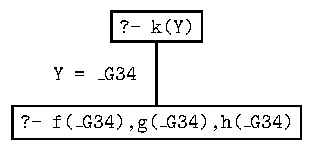
\includegraphics{chap2-pspic1.ps}
\end{center}
%
Everything in a box is either a query or a goal.  In particular, our
original goal was to prove �k(Y)�, thus this is shown in the top box.
When we unified �k(Y)� with the head of the rule in the knowledge
base, �X� �Y�, and the new internal variable �_G34� were made to share
values, and we were left with the goals �f(_G34),g(_G34),h(_G34)�,
just as shown.

Now, whenever it has a list of goals, Prolog tries to satisfy them one
by one, working through the list in a left to right direction. The
leftmost goal is �f(_G34)�, which reads: ``I want an individual with
property �f�''. Can this goal be satisfied? Prolog tries to do so by
searching through the knowledge base from top to bottom.  The first
item it finds that unifies with this goal is the fact �f(a)�. This
satisfies the goal �f(_G34)� and we are left with two more goals.
Now, when we unify �f(_G34)� to �f(a)�, �_G34� is instantiated to �a�,
and this instantiation applies to all occurrences of �_G34� in the
list of goals. So the list now looks like this:
\begin{LPNcodedisplay}
g(a),h(a)
\end{LPNcodedisplay}
%
and our graphical representation of the proof search now looks like this:
%
\begin{center}
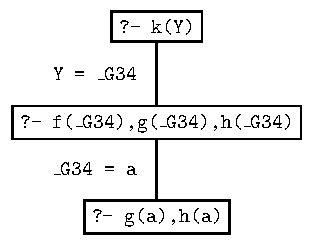
\includegraphics{chap2-pspic2.ps}
\end{center}
%

But the fact �g(a)� is in the knowledge base, so the first goal we
have to prove is satisfied too. So the goal list becomes
\begin{LPNcodedisplay}
h(a)
\end{LPNcodedisplay}
%
and the graphical representation is now
%
\begin{center}
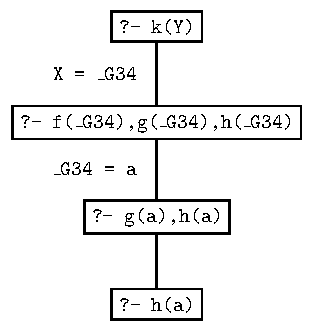
\includegraphics{chap2-pspic3.ps}
\end{center}
%
But there is no way to satisfy �h(a)�, the last remaining goal.  The
only information about �h� we have in the knowledge base is �h(b)�,
and this won't unify with �h(a)�.

So what happens next? Well, Prolog decides it has made a mistake, and
checks whether it has missed any possible ways of unifying a goal with
a fact or the head of a rule in the knowledge base. It does this by
going back up the path shown in the graphical representation, looking
for alternatives. Now, there is nothing else in the knowledge base
that unifies with �g(a)�, but there \LPNemph{is} another way of
unifying �f(_G34)�.  Points in the search where there are several
alternative ways of unifying a goal against the knowledge base are
called \LPNterm{choice points}.  Prolog keeps track of choice points it
has encountered, so that if it makes a wrong choice it can retreat to
the previous choice point and try something else instead. This process
is called \LPNterm{backtracking}, and it is fundamental to proof search
in Prolog.

So let's carry on with our example.
Prolog backtracks to the last choice point. This is the
point in the graphical representation where the list of goals was:
\begin{LPNcodedisplay}
f(_G34),g(_G34),h(_G34).
\end{LPNcodedisplay}
Prolog must now redo this work.  First it must try to
\LPNterm{re-satisfy} the first goal  by searching further in the
knowledge base.  It can do this: it sees that it can unify the first
goal with information in the knowledge base by unifying �f(_G34)� with
�f(b)�. This satisfies the goal �f(_G34)� and instantiates �X� to �b�,
so that the remaining goal list is
\begin{LPNcodedisplay}
g(b),h(b).
\end{LPNcodedisplay}
But �g(b)� is a fact in the knowledge base, so this is satisfied too,
leaving the goal list:
\begin{LPNcodedisplay}
h(b).
\end{LPNcodedisplay}
Moreover, this fact too is in the knowledge base, so this goal is also
satisfied. So Prolog now has an empty list of goals.  This means that
it has now proved everything required to establish the original goal
(that is, �k(Y)�). So the original query \LPNemph{is} satisfiable, and
moreover, Prolog has also discovered what it has to do to satisfy it
(namely instantiate �Y� to �b�).


It is interesting to consider what happens if we then ask for another
solution by typing:
\begin{LPNcodedisplay}
;
\end{LPNcodedisplay}
This forces Prolog to backtrack to the last choice point, to try and
find another possibility. However, there are no other choice points, as
there are no other possibilities for unifying �h(b)�, �g(b)�,
�f(_G34)�, or �k(Y)� with clauses in the knowledge base, so Prolog
would respond no.  On the other hand, if there had been other rules
involving �k�, Prolog would have gone off and tried to use them in
exactly the way we have described: that is, by searching top to bottom
in the knowledge base, left to right in goal lists, and backtracking
to the previous choice point whenever it fails.


Let's take a look at the graphical representation of the entire search
process. Some general remarks are called for, for such representations
are an important way of thinking about proof search in Prolog.
%
\begin{center}
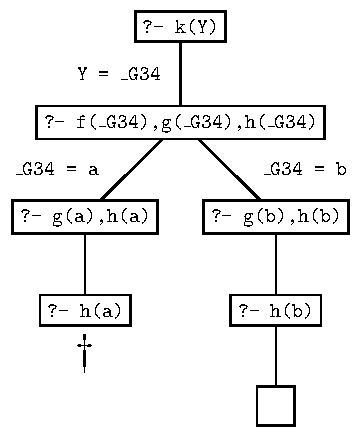
\includegraphics{chap2-pspic4.ps}
\end{center}
This diagram has the form of a tree; in fact it is our first example
of what is known as a \LPNterm{search tree}.  The nodes of such trees
say which goals have to be satisfied at the various steps of the proof
search, and the edges keep track of the variable instantiations that
are made when the current goal (that is, the first one in the list of
goals) is unified to a fact or to the head of a rule in the knowledge
base.  Leaf nodes which still contain unsatisfied goals are points
where Prolog failed (either because it made a wrong decision somewhere
along the path, or because no solution exists). Leaf nodes with an
empty goal list correspond to a possible solution.  The edges along
the path from the root node to a successful leaf node tell you the
variable instantiations that need to be made to satisfy the original
query.

Let's have a look at another example. Suppose that we are working with
the following knowledge base:
\begin{LPNcodedisplay}
loves(vincent,mia).
loves(marcellus,mia).

jealous(A,B):- loves(A,C), loves(B,C).
\end{LPNcodedisplay}
%
Now we pose the query
\begin{LPNcodedisplay}
?- jealous(X,Y).
\end{LPNcodedisplay}
%
The search tree for the query looks like this:
%
\begin{center}
\includegraphics{chap2-pspic5.ps}
\end{center}

There is only one possible way of unifying �jealous(X,Y)� against the
knowledge base, namely by using the rule
\begin{LPNcodedisplay}
jealous(A,B):- loves(A,C), loves(B,C).
\end{LPNcodedisplay}
%
So the new goals that have to be satisfied are:
\begin{LPNcodedisplay}
loves(_G5,_G6),loves(_G7,_G6)
\end{LPNcodedisplay}
Now we have to unify �loves(_G5,_G6)� against the knowledge base.
There are two ways of doing this (it can either be unified with the
first fact or with the second fact) and this is why the path branches
at this point. In both cases the goal �loves(_G7,mia)� remains, and
this can also be satisfied by using  either of two facts.  All in
all there are four leaf nodes with an empty goal list, which means
that there are four ways of satisfying the original query. The
variable instantiations for each solution can be read off the path
from the root to the leaf node. So the four solutions are:
\begin{enumerate}
\item{}�X = _G5 = vincent� and
�Y = _G7 = vincent�
\item{}�X = _G5 = vincent� and
�Y = _G7 = marcellus�
\item{}�X = _G5 = marcellus� and
�Y = _G7 = vincent�
\item{}�X = _G5 = marcellus� and
�Y = _G7 = marcellus�
\end{enumerate}
Work through this example carefully, and make sure you understand it.

%\pagebreak
\section{Exercises}\label{SEC.L2.EXERCISES}

\begin{LPNexercise}{L2.EX1}Which of the following pairs of terms unify?
Where relevant, give the
variable instantiations that lead to successful unification.
\begin{enumerate}
\item{}�bread = bread�
\item{}�'Bread' = bread�
\item{}�'bread' = bread�
\item{}�Bread = bread�
\item{}�bread = sausage�
\item{}�food(bread) = bread�
\item{}�food(bread) = X�
\item{}�food(X) = food(bread)�
\item{}�food(bread,X) = food(Y,sausage)�
\item{}�food(bread,X,beer) = food(Y,sausage,X)�
\item{}�food(bread,X,beer) = food(Y,kahuna_burger)�
\item{}�food(X) = X�
\item{}�meal(food(bread),drink(beer)) = meal(X,Y)�
\item{}�meal(food(bread),X) = meal(X,drink(beer))�
\end{enumerate}
\end{LPNexercise}

\begin{LPNexercise}{L2.EX2}We are working with the following knowledge base:
\begin{LPNcodedisplay}
house_elf(dobby).
witch(hermione).
witch('McGonagall').
witch(rita_skeeter).
magic(X):- house_elf(X).
magic(X):- wizard(X).
magic(X):- witch(X).
\end{LPNcodedisplay}


Which of the following queries are satisfied? Where relevant, give all
the variable instantiations that lead to success.
\begin{enumerate}
\item{}�?- magic(house_elf).�
\item{}�?- wizard(harry).�
\item{}�?- magic(wizard).�
\item{}�?- magic('McGonagall').�
\item{}�?- magic(Hermione).�
\end{enumerate}
Draw the search tree for the query �magic(Hermione)�.
\end{LPNexercise}


\begin{LPNexercise}{L2.EX3}Here is a tiny lexicon
(that is, information about individual words) and a mini grammar
consisting of one syntactic rule (which defines a sentence to be an
entity consisting of five words in the following order: a determiner,
a noun, a verb, a determiner, a noun).

\begin{LPNcodedisplay}
word(determiner,a).
word(determiner,every).
word(noun,criminal).
word(noun,'big kahuna burger').
word(verb,eats).
word(verb,likes).

sentence(Word1,Word2,Word3,Word4,Word5):-
   word(determiner,Word1),
   word(noun,Word2),
   word(verb,Word3),
   word(determiner,Word4),
   word(noun,Word5).
\end{LPNcodedisplay}
What query do you have to pose in order to find out which sentences
the grammar can generate?  List all sentences that this grammar can
generate in the order that Prolog will generate them in.
\end{LPNexercise}



\begin{LPNexercise}{L2.EX4}Here are six Italian words:

\LPNemph{astante}, \LPNemph{astoria}, \LPNemph{baratto},
\LPNemph{cobalto}, \LPNemph{pistola}, \LPNemph{statale}.

\noindent
They are to be arranged, crossword puzzle
fashion, in the following grid:

\bigskip
\begin{center}
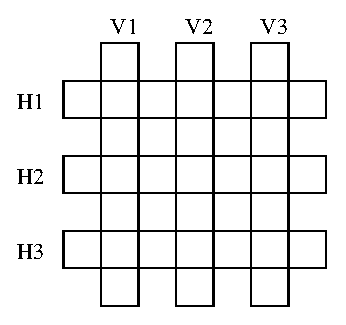
\includegraphics{crosswd2.eps}
\end{center}
\bigskip

The following knowledge base represents a lexicon containing these
words:
\begin{LPNcodedisplay}
word(astante, a,s,t,a,n,t,e).
word(astoria, a,s,t,o,r,i,a).
word(baratto, b,a,r,a,t,t,o).
word(cobalto, c,o,b,a,l,t,o).
word(pistola, p,i,s,t,o,l,a).
word(statale, s,t,a,t,a,l,e).
\end{LPNcodedisplay}
Write a predicate �crossword/6� that tells us how to fill in the grid.
The first three arguments should be the vertical words from left to
right, and the last three arguments the horizontal words from top
to bottom.\end{LPNexercise}


\section{Practical Session}\label{SEC.L2.PRAXIS}


By this stage, you should have had your first taste of running Prolog
programs. The purpose of the second practical session is to suggest
two sets of keyboard exercises which will help you get familiar with
the way Prolog works. The first set has to do with unification, the
second with proof search.

First of all, start up your Prolog interpreter. That is, get a screen
displaying the usual ``I'm ready to start'' prompt, which probably looks
something like:
\begin{LPNcodedisplay}
?-
\end{LPNcodedisplay}
Verify your answers to Exercise 2.1, the unification examples. You
don't need to consult any knowledge bases, simply ask Prolog directly
whether it is possible to unify the terms by using the built-in �=/2�
predicate. For example, to test whether �food(bread,X)� and
�food(Y,sausage)� unify, just type in
\begin{LPNcodedisplay}
food(bread,X) = food(Y,sausage).
\end{LPNcodedisplay}
%
and hit return.

You should also look at what happens when your Prolog implementation
attempts to unify terms that can't be unified because it doesn't carry
out an occurs check. For example, see what happens when you give it
the following query:
\begin{LPNcodedisplay}
g(X,Y) = Y.
\end{LPNcodedisplay}
If it handles such examples, try the trickier one mentioned in the
text:
\begin{LPNcodedisplay}
X = f(X), Y = f(Y), X = Y.
\end{LPNcodedisplay}

Once you've experimented with that, it's time to move on to something
new.  There is another built-in Prolog predicate for
answering queries about unification, namely �\=/2� (that is: the
2-place predicate �\=�).  \index{PROLOG \=/2@\verb-\=/2-} This works
in the opposite way to the �=/2� predicate: it succeeds when its two
arguments do \LPNemph{not} unify.  For example, the terms �a� and �b�
do not unify, which explains the following dialogue:
\begin{LPNcodedisplay}
?- a \= b.
yes
\end{LPNcodedisplay}

Make sure you understand how  �\=/2� works by trying it
out on (at least) the following examples.  But do this actively, not
passively.  That is, after you type in an example, pause, and try to
work out for yourself what Prolog is going to respond. Only then hit
return to see if you are right.
\begin{enumerate}
\item{}�a \= a�
\item{}�'a' \= a�
\item{}�A \= a�
\item{}�f(a) \= a�
\item{}�f(a) \= A�
\item{}�f(A) \= f(a)�
\item{}�g(a,B,c) \= g(A,b,C)�
\item{}�g(a,b,c) \= g(A,C)�
\item{}�f(X) \= X�
\end{enumerate}

Thus the �\=/2� predicate is (essentially) the negation of
the �=/2� predicate: a query involving one of these predicates will be
satisfied when the corresponding query involving the other is not, and
vice versa. This is the first example we have seen of a Prolog
mechanism for handling negation.  We discuss Prolog negation (and its
peculiarities) in Chapter~\ref{CHAPTER10}.

It's time to move on and introduce one of the most helpful tools in
Prolog: �trace�.\index{PROLOG trace/0@\texttt{trace/0}} This is a built-in
Prolog predicate that changes the
way Prolog runs: it forces Prolog to evaluate queries one step at a
time, indicating what it is doing at each step. Prolog waits for you
to press return before it moves to the next step, so that you can see
exactly what is going on. It was really designed to be used as a
debugging tool, but it's also helpful when you're learning
Prolog: stepping through programs using �trace� is an
\LPNemph{excellent} way of learning how Prolog proof search works.

Let's look at an example.  In the text, we looked at the proof
search involved when we made the query �k(Y)� to the following
knowledge base:
\begin{LPNcodedisplay}
f(a).
f(b).

g(a).
g(b).

h(b).

k(X):- f(X), g(X), h(X).
\end{LPNcodedisplay}

Suppose this knowledge base is in file �proof.pl�. We first consult
it:
\begin{LPNcodedisplay}
?- [proof].
yes
\end{LPNcodedisplay}
%
We then type �trace�, followed by a full stop,  and hit return:
\begin{LPNcodedisplay}
?- trace.
yes
\end{LPNcodedisplay}
%
Prolog is now in \LPNterm{trace mode}, and will evaluate all queries step by
step.  For example, if we pose the query �k(X)�, and then hit return
every time Prolog comes back with a �?�, we obtain (something like)
the following:
\begin{LPNcodedisplay}
[trace] 2 ?- k(X).
   Call: (6) k(_G34) ?
   Call: (7) f(_G34) ?
   Exit: (7) f(a) ?
   Call: (7) g(a) ?
   Exit: (7) g(a) ?
   Call: (7) h(a) ?
   Fail: (7) h(a) ?
   Fail: (7) g(a) ?
   Redo: (7) f(_G34) ?
   Exit: (7) f(b) ?
   Call: (7) g(b) ?
   Exit: (7) g(b) ?
   Call: (7) h(b) ?
   Exit: (7) h(b) ?
   Exit: (6) k(b) ?

X = b
yes
\end{LPNcodedisplay}

Study this carefully. That is, try doing the same thing yourself, and
relate this output to the discussion of the example in the text, and
in particular, to the nodes in the search tree.  To get you started,
we'll remark that the third line is where the variable in the query is
(wrongly) instantiated to �a�. The first line marked �fail� is where
Prolog realises it's taken the wrong path and starts to backtrack, and
the line marked �redo� is where it tries alternatives for the goal
�f(_G34)�.

\clearpage
While learning Prolog, use trace, and use it heavily. It's a great way
to learn.
Oh yes: you also need to know how to turn trace off. Simply type
notrace\index{PROLOG notrace/0@\texttt{notrace/0}} (followed by a full
stop) and hit return:
\begin{LPNcodedisplay}
?- notrace.
yes
\end{LPNcodedisplay}



\chapter{Recursion}\label{CHAPTER3}

\Thischapter{120}{

\noindent
This chapter has two main goals:

\begin{enumerate}
\item{}To introduce recursive definitions in Prolog.


\item{}To show that there can be mismatches between the
      declarative meaning of a Prolog program, and its
      procedural meaning.

\end{enumerate}

}

\section{Recursive Definitions}\label{SEC.L3.RECURSIVE.DEFINITION}



Predicates can be defined recursively.  Roughly speaking, a predicate
is recursively defined if one or more rules in its definition refers
to itself.

\subsection*{Example 1: Eating}\label{SUBSEC.L3.EX1}



Consider the following knowledge base:
\begin{LPNcodedisplay}
is_digesting(X,Y) :- just_ate(X,Y).
is_digesting(X,Y) :-
        just_ate(X,Z),
        is_digesting(Z,Y).

just_ate(mosquito,blood(john)).
just_ate(frog,mosquito).
just_ate(stork,frog).
\end{LPNcodedisplay}


At first glance this seems pretty ordinary: it's just a knowledge base
containing three facts and two rules.  But the definition of the
�is_digesting/2� predicate is \LPNterm{recursive}.  Note that
�is_digesting/2� is (at least partially) defined in terms of itself,
for the �is_digesting/2� functor occurs in both the head and body of
the second rule.  Crucially, however, there is an `escape' from this
circularity.  This is provided by the �just_ate/2� predicate, which
occurs in the first rule.  (Significantly, the body of the first rule
makes no mention of �is_digesting/2�.)  Let's now consider both the
\LPNterm{declarative} and \LPNterm{procedural} meanings of this definition.

The word ``declarative'' is used to talk about the logical meaning of
Prolog knowledge bases.  That is, the declarative meaning of a Prolog
knowledge base is simply ``what it says'', or ``what it means, if we read
it as a collection of logical statements''.  And the declarative
meaning of this recursive definition is fairly straightforward.  The
first clause (the escape clause, the one that is not recursive, or
as we shall usually call it, the \LPNterm{base clause}), simply says
that: \LPNemph{if} �X� has just eaten �Y�, \LPNemph{then} �X� is now
digesting �Y�.  This is obviously a sensible definition.

So what about the second clause, the \LPNterm{recursive clause}?  This
says that: \LPNemph{if} �X� has just eaten �Z�
\LPNemph{and} �Z� is digesting �Y�, \LPNemph{then} �X�
is digesting �Y�, too. Again, this is obviously a sensible
definition.

So now we know what this recursive definition says, but what happens
when we pose a query that actually needs to use this definition?  That
is, what does this definition actually do?  To use the normal Prolog
terminology, what is its procedural meaning?

This is also reasonably straightforward.  The base rule is like all
the earlier rules we've seen.  That is, if we ask whether �X� is
digesting �Y�, Prolog can use this rule to ask instead
the question: has �X� just eaten �Y�?

What about the recursive clause?  This gives Prolog another strategy
for determining whether �X� is digesting �Y�:
\LPNemph{it can try to find some} �Z� \LPNemph{such that} �X�
\LPNemph{has just eaten} �Z�, and �Z� \LPNemph{is digesting}
�Y�.  That is, this rule lets Prolog break the task
apart into two subtasks.  Hopefully, doing so will eventually lead to
simple problems which can be solved by simply looking up the answers
in the knowledge base. The following picture sums up the situation:

\medskip

\begin{center}
\includegraphics{chap3-pspic3.ps}
\end{center}

Let's see how this works. If we pose the query:
\begin{LPNcodedisplay}
?- is_digesting(stork,mosquito).
\end{LPNcodedisplay}
then Prolog goes to work as follows.  First, it tries to make use of
the first rule listed concerning �is_digesting�; that is, the
base rule.  This tells it that �X� is digesting
�Y� if �X� just ate �Y�, By unifying
�X� with �stork� and �Y� with
�mosquito� it obtains the following goal:
\begin{LPNcodedisplay}
just_ate(stork,mosquito).
\end{LPNcodedisplay}


But the knowledge base doesn't contain the information that the stork
just ate the mosquito, so this
attempt fails.  So Prolog next tries to make use of the second rule.
By unifying �X� with �stork� and �Y� with
�mosquito� it obtains the following goals:
\begin{LPNcodedisplay}
just_ate(stork,Z),
is_digesting(Z,mosquito).
\end{LPNcodedisplay}
That is, to show
�is_digesting(stork,mosquito)�, Prolog
needs to find a value for �Z� such that, firstly,
\begin{LPNcodedisplay}
just_ate(stork,Z).
\end{LPNcodedisplay}
and secondly,
\begin{LPNcodedisplay}
is_digesting(Z,mosquito).
\end{LPNcodedisplay}
And there \LPNemph{is} such a value for �Z�, namely
�frog�.  It is immediate that
\begin{LPNcodedisplay}
just_ate(stork,frog).
\end{LPNcodedisplay}
will succeed, for this fact is listed in the knowledge base.  And deducing
\begin{LPNcodedisplay}
is_digesting(frog,mosquito).
\end{LPNcodedisplay}
is almost as simple, for the first clause of �is_digesting/2�
reduces this goal to deducing
\begin{LPNcodedisplay}
just_ate(frog,mosquito).
\end{LPNcodedisplay}
and this is a fact listed in the knowledge base.

Well, that's our first example of a recursive rule definition.  We're
going to learn a lot more about them, but one very practical remark
should be made right away.  Hopefully it's clear that when you write a
recursive predicate, it should always have at least two clauses: a
base clause (the clause that stops the recursion at some point), and
one that contains the recursion.  If you don't do this, Prolog can
spiral off into an unending sequence of useless computations.  For
example, here's an extremely simple example of a recursive rule
definition:
\begin{LPNcodedisplay}
p :- p.
\end{LPNcodedisplay}
That's it.  Nothing else.  It's beautiful in its simplicity.  And from
a declarative perspective it's an extremely sensible (if rather
boring) definition: it says ``if property p holds, then property
p holds''. You can't argue with that.

But from a procedural perspective, this is a wildly dangerous rule. In
fact, we have here the ultimate in dangerous recursive rules: exactly
the same thing on both sides, and no base clause to let us escape.
For consider what happens when we pose the following query:
\begin{LPNcodedisplay}
?- p.
\end{LPNcodedisplay}
Prolog asks itself: ``How do I prove �p�?''  and it realises, ``Hey,
I've got a rule for that!  To prove �p� I just need to prove �p�!''.
So it asks itself (again): ``How do I prove �p�?''  and it realises,
``Hey, I've got a rule for that!  To prove �p� I just need to prove
�p�!''.  So it asks itself (yet again): ``How do I prove �p�?''  and
it realises, ``Hey, I've got a rule for that!  To prove �p� I just
need to prove �p�!''  and so on and so forth.

If you make this query, Prolog won't answer you: it will head off,
looping desperately away in an unending search.  That is, it won't
terminate, and you'll have to interrupt it. Of course, if you use
�trace�, you can step through one step at a time, until you get
sick of watching Prolog loop.

\subsection*{Example 2: Descendant}\label{SUBSEC.L3.EX2}



Now that we know something about \LPNemph{what} recursion in Prolog
involves, it is time to ask \LPNemph{why} it is so important.  Actually,
this is a question that can be answered on a number of levels, but for
now, let's keep things fairly practical.  So: when it comes to writing
useful Prolog programs, are recursive definitions really so important?
And if so, why?

Let's consider an example.  Suppose we have a knowledge base recording
facts about the child relation:
\begin{LPNcodedisplay}
child(bridget,caroline).
child(caroline,donna).
\end{LPNcodedisplay}
That is, Caroline is a child of Bridget, and Donna is a child of
Caroline. Now suppose we wished to define the descendant relation;
that is, the relation of being a child of, or a child of a child of,
or a child of a child of a child of, and so on.  Here's a first attempt to
do this.  We could add the following two \LPNemph{non}-recursive rules to
the knowledge base:
\begin{LPNcodedisplay}
descend(X,Y) :- child(X,Y).

descend(X,Y) :- child(X,Z),
                 child(Z,Y).
\end{LPNcodedisplay}


Now, fairly obviously these definitions work up to a point, but they are
clearly limited: they only define the concept of
descendant-of for two generations or less.  That's ok for the above
knowledge base, but suppose we get some more information about the
child-of relation and we expand our list of child-of facts to this:
\begin{LPNcodedisplay}
child(anne,bridget).
child(bridget,caroline).
child(caroline,donna).
child(donna,emily).
\end{LPNcodedisplay}

Now our two rules are inadequate.  For example, if we pose the queries
\begin{LPNcodedisplay}
?- descend(anne,donna).
\end{LPNcodedisplay}
or
\begin{LPNcodedisplay}
?- descend(bridget,emily).
\end{LPNcodedisplay}
we get the answer no, which is \LPNemph{not} what we want.  Sure,
we could `fix' this by adding the following two rules:
\begin{LPNcodedisplay}
descend(X,Y) :- child(X,Z_1),
                 child(Z_1,Z_2),
                 child(Z_2,Y).

descend(X,Y) :- child(X,Z_1),
                 child(Z_1,Z_2),
                 child(Z_2,Z_3),
                 child(Z_3,Y).
\end{LPNcodedisplay}

But, let's face it, this is clumsy and hard to read.  Moreover, if we
add further child-of facts, we could easily find ourselves having to
add more and more rules as our list of child-of facts grow, rules
like:
\begin{LPNcodedisplay}
descend(X,Y) :- child(X,Z_1),
                 child(Z_1,Z_2),
                 child(Z_2,Z_3),
                                        .
                     .
                     .
                 child(Z_17,Z_18).
                 child(Z_18,Z_19).
                 child(Z_19,Y).
\end{LPNcodedisplay}
This is not a particularly pleasant (or sensible) way to go!

But we don't need to do this at all. We can avoid
having to use ever longer rules entirely. The
following  recursive predicate definition fixes everything exactly
the way we want:
\begin{LPNcodedisplay}
descend(X,Y) :- child(X,Y).

descend(X,Y) :- child(X,Z),
                 descend(Z,Y).
\end{LPNcodedisplay}



What does this say?  The declarative meaning of the base clause
is: \LPNemph{if} �Y� is a child of �X�, \LPNemph{then} �Y� is a
descendant of �X�. Obviously sensible.
So what about the recursive clause?  Its declarative meaning is:
\LPNemph{if} �Z� is a child of �X�, \LPNemph{and} �Y� is a
descendant of �Z�, \LPNemph{then} �Y� is a descendant of
�X�. Again, this is obviously true.

So let's now look at the procedural meaning of this recursive
predicate, by stepping through an example. What happens when we pose
the query:
\begin{LPNcodedisplay}
descend(anne,donna)
\end{LPNcodedisplay}
Prolog first tries the first rule. The variable �X� in the head
of the rule is unified with �anne� and �Y� with �donna�  and
the next goal Prolog tries to prove is

\begin{LPNcodedisplay}
child(anne,donna)
\end{LPNcodedisplay}


This attempt fails, however, since the knowledge base
neither contains the fact �child(anne,donna)� nor any rules
that would allow to infer it.
So Prolog backtracks and looks for an alternative way of proving
�descend(anne,donna)�. It finds the second rule in the
knowledge base and now has the following subgoals:

\begin{LPNcodedisplay}
child(anne,_633),
descend(_633,donna).
\end{LPNcodedisplay}


Prolog takes the first subgoal and tries to unify  it with something in
the knowledge base. It finds the fact �child(anne,bridget)�
and the variable �_633� gets instantiated to �bridget�.
Now that the first subgoal is satisfied, Prolog moves to the
second subgoal. It has to prove

\begin{LPNcodedisplay}
descend(bridget,donna)
\end{LPNcodedisplay}


This is the first recursive call of the predicate �descend/2�. As
before, Prolog starts with the first rule, but fails, because the goal

\begin{LPNcodedisplay}
child(bridget,donna)
\end{LPNcodedisplay}
cannot be proved. Backtracking, Prolog finds that there is a second
possibility to be checked for �descend(bridget,donna)�, namely the
second rule, which again gives Prolog two new subgoals:

\begin{LPNcodedisplay}
child(bridget,_1785),
descend(_1785,donna).
\end{LPNcodedisplay}


The first one can be unified with the fact
�child(bridget,caroline)� of the knowledge base, so that the
variable �_1785� is instantiated with �caroline�. Next Prolog
tries to prove

\begin{LPNcodedisplay}
descend(caroline,donna).
\end{LPNcodedisplay}
This is the second recursive call of predicate �descend/2�.
As before, it tries the first rule first, obtaining the following new
goal:

\begin{LPNcodedisplay}
child(caroline,donna)
\end{LPNcodedisplay}


This time Prolog succeeds, since �child(caroline,donna)� is a
fact in the database. Prolog has found a proof for the goal
�descend(caroline,donna)� (the second recursive call). But this
means that �descend(bridget,donna)� (the first recursive call)
is also true, which means that our original query
�descend(anne,donna)� is true as well.

Here is the search tree for the query
�descend(anne,donna)�. Make sure that you understand how it
relates to the discussion in the text; that is, how Prolog
traverses this search tree when trying to prove this query.

\begin{center}
\includegraphics{chap3-pspic1.ps}
\end{center}

\bigskip
\bigskip
\bigskip
\medskip

It should be obvious from this example that no matter how many
generations of children we add, we will always be able to work out the
descendant relation. That is, the recursive definition is both general
and compact: it contains \LPNemph{all} the information in the
non-recursive rules, and much more besides.  The non-recursive rules
only defined the descendant concept up to some fixed number of
generations: we would need to write down infinitely many non-recursive
rules if we wanted to capture this concept fully, and of course that's
impossible.  But, in effect, that's what the recursive rule does for
us: it bundles up the information needed to cope with arbitrary
numbers of generations into just three lines of code.

Recursive rules are really important. They enable to pack an enormous
amount of information into a compact form and to define predicates in
a natural way.  Most of the work you will do as a Prolog programmer
will involve writing recursive rules.

\subsection*{Example 3: Successor}\label{SUBSEC.L3.EX3}



In the previous chapter we remarked that building structure through
unification is a key idea in Prolog programming.  Now that we know
about recursion, we can give more interesting illustrations of this.

Nowadays, when human beings write numerals, they usually use
\LPNemph{decimal} notation (0, 1, 2, 3, 4, 5, 6, 7, 8, 9, 10, 11, 12, and
so on) but as you probably know, there are many other notations.  For
example, because computer hardware is generally based on digital
circuits, computers usually use \LPNemph{binary} notation to represent
numerals (0, 1, 10, 11, 100, 101, 110, 111, 1000, and so on), for the
0 can be implemented as a switch being off, the 1 as a switch being
on.  Other cultures use different systems.  For example, the
ancient Babylonians used a base 60 system, while the ancient Romans
used a rather ad-hoc system (I, II, III, IV, V, VI, VII, VIII, IX, X).
This last example shows that notational issues can be important.  If
you don't believe this, try figuring out a systematic way of doing
long-division in Roman notation.  As you'll discover, it's a
frustrating task.  Apparently the Romans had a group of professionals
(analogs of modern accountants) who specialised in this.

Well, here's yet another way of writing numerals, which is
sometimes used in mathematical logic.  It makes use of just four
symbols: 0, \LPNemph{succ}, and the left and right parentheses.  This style
of numeral is defined by the following inductive definition:
\begin{enumerate}
\item{}0 is a numeral.

\item{}If \LPNemph{X} is a numeral, then so is \LPNemph{succ(X)}.
\end{enumerate}


As is probably clear, \LPNemph{succ} can be read as short for
\LPNemph{successor}. That is, \LPNemph{succ(X)} represents the number obtained by
adding one to the number represented by \LPNemph{X}.  So this is a very
simple notation: it simply says that 0 is a numeral, and that all
other numerals are built by stacking \LPNemph{succ} symbols in front.  (In
fact, it's used in mathematical logic because of this simplicity.
Although it wouldn't be pleasant to do household accounts in this
notation, it is a very easy notation to prove things \LPNemph{about}.)

Now, by this stage it should be clear that we can turn this
definition into a Prolog program.  The following knowledge base does
this:
\begin{LPNcodedisplay}
numeral(0).

numeral(succ(X)) :- numeral(X).
\end{LPNcodedisplay}
So if we pose queries like
\begin{LPNcodedisplay}
numeral(succ(succ(succ(0)))).
\end{LPNcodedisplay}
we get the answer yes.

But we can do some more interesting things.  Consider what happens when
we pose the following query:
\begin{LPNcodedisplay}
numeral(X).
\end{LPNcodedisplay}
That is, we're saying ``Ok, show me some numerals''.  Then we can have
the following dialogue with Prolog:
\begin{LPNcodedisplay}
X = 0 ;

X = succ(0) ;

X = succ(succ(0)) ;

X = succ(succ(succ(0))) ;

X = succ(succ(succ(succ(0)))) ;

X = succ(succ(succ(succ(succ(0))))) ;

X = succ(succ(succ(succ(succ(succ(0)))))) ;

X = succ(succ(succ(succ(succ(succ(succ(0))))))) ;

X = succ(succ(succ(succ(succ(succ(succ(succ(0))))))))
yes
\end{LPNcodedisplay}


Yes, Prolog is counting: but what's really important is \LPNemph{how} it's
doing this. Quite simply, it's backtracking through the recursive
definition, and actually \LPNemph{building} numerals using unification. This
is an instructive example, and it is important that you understand
it. The best way to do so is to sit down and try it out, with
�trace� turned on.

Building and binding.  Recursion, unification, and proof search.  These
are ideas that lie at the heart of Prolog programming.  Whenever we
have to generate or analyse recursively structured objects (such as
these numerals) the interplay of these ideas makes Prolog a powerful
tool.  For example, in the next chapter we shall introduce
\LPNterm{lists}, an extremely important recursive data structure, and
we will see that Prolog is a natural list processing language.  Many
applications (computational linguistics is a prime example) make heavy
use of recursively structured objects, such as trees and feature
structures.  So it's not particularly surprising that Prolog has
proved useful in such applications.

\subsection*{Example 4: Addition}\label{SUBSEC.L3.EX4}



As a final example, let's see whether we can use the representation of
numerals that we introduced in the previous section for doing simple
arithmetic. Let's try to define addition. That is, we want to define a
predicate �add/3� which when given two numerals as the
first and second argument returns the result of adding them up as its
third argument. For example:
\begin{LPNcodedisplay}
?- add(succ(succ(0)),succ(succ(0)),
       succ(succ(succ(succ(0))))).
yes
?- add(succ(succ(0)),succ(0),Y).
Y = succ(succ(succ(0)))
\end{LPNcodedisplay}

There are two things which are important to notice:
\begin{enumerate}
\item{}Whenever the first argument is �0�, the third argument has
to be the same as the second argument:
\begin{LPNcodedisplay}
?- add(0,succ(succ(0)),Y).
Y = succ(succ(0))
?- add(0,0,Y).
Y = 0
\end{LPNcodedisplay}

This is the case that we want to use for the base clause.
\item{}Assume that we want to add the two numerals �X� and �Y�
(for example  �succ(succ(succ(0)))� and �succ(succ(0))�) and that
�X� is not �0�. Now, if
�X1� is the numeral that has one �succ� functor less than
�X� (that is, �succ(succ(0))� in our example) and if we know the
result -- let's call it �Z� -- of adding �X1� and �Y�
(namely �succ(succ(succ(succ(0))))�), then it is very easy to
compute the result of adding �X� and �Y�: we just have to
add one �succ�-functor to �Z�. This is what we want to
express with the recursive clause.
\end{enumerate}

Here is the predicate definition that expresses exactly what we just said:
\begin{LPNcodedisplay}
add(0,Y,Y).
add(succ(X),Y,succ(Z)) :-
        add(X,Y,Z).
\end{LPNcodedisplay}

So what happens, if we give Prolog this predicate definition and then
ask:
\begin{LPNcodedisplay}
?- add(succ(succ(succ(0))), succ(succ(0)), R).
\end{LPNcodedisplay}
 Let's go step by step through the way Prolog processes this
query. The trace and search tree for the query are given below.

The first argument is not �0�, which means that only the second clause
for �add/3� can be used. This leads to a recursive call of �add/3�. The
outermost �succ� functor is stripped off the first argument of the
original query, and the result becomes the first argument of the
recursive query. The second argument is passed on unchanged to the
recursive query, and the third argument of the recursive query is a
variable, the internal variable �_G648� in the trace given below. Note
that �_G648� is not instantiated yet. However it shares values with
�R� (the variable that we used as the third argument in the original
query) because �R� was instantiated to �succ(_G648)� when the query
was unified with the head of the second clause. But that means that
�R� is not a completely uninstantiated variable anymore. It is now a
complex term, that has a (uninstantiated) variable as its argument.

The next two steps are essentially the same. With every step the first
argument becomes one layer of �succ� smaller; both the trace and the
search tree given below show this nicely.  At the same time, a �succ�
functor is added to �R� at every step, but always leaving
the innermost variable uninstantiated. After the first recursive
call �R� is �succ(_G648)�.  After the second recursive call, �_G648�
is instantiated with �succ(_G650)�, so that �R� is �succ(succ(_G650)�.
After the third recursive call, �_G650� is instantiated with
�succ(_G652)� and �R� therefore becomes �succ(succ(succ(_G652)))�. The
search tree shows this step by step instantiation.

At this stage all �succ� functors have been stripped off the first
argument and we can apply the base clause. The third argument is
equated with the second argument, so the  `hole' (the
uninstantiated variable) in the complex term �R� is finally filled,
and we are through.

Here's the complete trace of our query:
\begin{LPNcodedisplay}
Call: (6) add(succ(succ(succ(0))), succ(succ(0)), R)

Call: (7) add(succ(succ(0)), succ(succ(0)), _G648)

Call: (8) add(succ(0), succ(succ(0)), _G650)

Call: (9) add(0, succ(succ(0)), _G652)

Exit: (9) add(0, succ(succ(0)), succ(succ(0)))

Exit: (8) add(succ(0), succ(succ(0)), succ(succ(succ(0))))

Exit: (7) add(succ(succ(0)), succ(succ(0)),
                                succ(succ(succ(succ(0)))))

Exit: (6) add(succ(succ(succ(0))), succ(succ(0)),
                          succ(succ(succ(succ(succ(0))))))
\end{LPNcodedisplay}

And here's the search tree:

\begin{center}
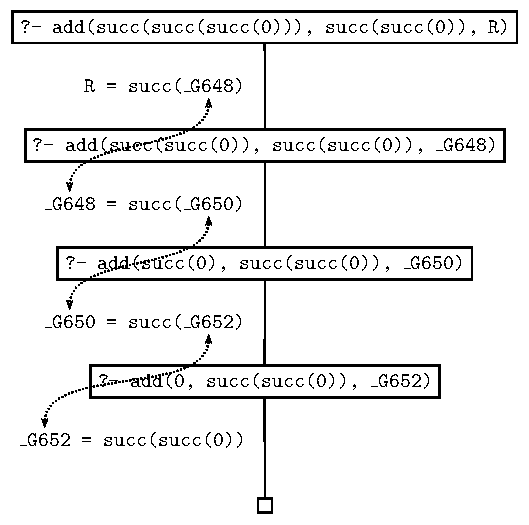
\includegraphics{chap3-pspic2.ps}
\end{center}

\section{Rule Ordering, Goal Ordering, and Termination}\label{SEC.L3.RO.CO.TERM}



Prolog was the first reasonably successful attempt to create a
\LPNterm{logic programming} language.  Underlying logic programming is
a simple (and seductive) vision: the task of the programmer is simply
to \LPNemph{describe} problems.  The programmer should write down (in
the language of logic) a declarative specification (that is: a
knowledge base), which describes the situation of interest.  The
programmer shouldn't have to tell the computer \LPNemph{what} to do.
To get information, he or she simply asks the questions.  It's up to
the logic programming system to figure out how to get the answer.

Well, that's the idea, and it should be clear that Prolog has taken
some important steps in this direction.  But Prolog is \LPNemph{not},
repeat \LPNemph{not}, a full logic programming language.  If you only
think about the declarative meaning of a Prolog program, you are in
for a very tough time.  As we learned in the previous chapter, Prolog
has a very specific way of working out the answers to queries: it
searches the knowledge base from top to bottom, clauses from left to
right, and uses backtracking to recover from bad choices. These
procedural aspects have an important influence on what actually
happens when you make a query. We have already seen a dramatic example
of a mismatch between the procedural and declarative meaning of a
knowledge base (remember the �p:- p� program?), and as we shall now
see, it is easy to define knowledge bases which (read logically)
describe the same situations, but which behave very differently.
Let's consider the matter.

Recall our earlier descendant program (let's call it �descend1.pl�):
\begin{LPNcodedisplay}
child(anne,bridget).
child(bridget,caroline).
child(caroline,donna).
child(donna,emily).

descend(X,Y) :- child(X,Y).

descend(X,Y) :- child(X,Z),
                 descend(Z,Y).
\end{LPNcodedisplay}


We'll make one change to it, and call the result �descend2.pl�:
\begin{LPNcodedisplay}
child(anne,bridget).
child(bridget,caroline).
child(caroline,donna).
child(donna,emily).

descend(X,Y) :- child(X,Z),
                 descend(Z,Y).

descend(X,Y) :- child(X,Y).
\end{LPNcodedisplay}

All we have done is change the \LPNterm{rule order}. So if we read the
program as a purely logical definition, nothing has changed.  But does
the change give rise to procedural differences?  Yes, but nothing
significant. For example, if you work through the examples you
will see that the first solution that �descend1.pl� finds is
\begin{LPNcodedisplay}
X = anne
Y = bridget
\end{LPNcodedisplay}
whereas the first solution that �descend2.pl� finds is
\begin{LPNcodedisplay}
X = anne
Y = emily
\end{LPNcodedisplay}
But (as you should check) both programs generate exactly the same
answers, they merely find them in a different order. And this is a
general point. Roughly speaking (we'll add a caveat later on) changing
the order of rules in a Prolog program does not change (up to the
order in which solutions are found) the program's behaviour.

So let's move on. We'll make one small change to �descend2.pl�, and
call the result �descend3.pl�:
\begin{LPNcodedisplay}
child(anne,bridget).
child(bridget,caroline).
child(caroline,donna).
child(donna,emily).

descend(X,Y) :- descend(Z,Y),
                 child(X,Z).

descend(X,Y) :- child(X,Y).
\end{LPNcodedisplay}

Note the difference. Here we've changed the \LPNterm{goal order}
\LPNemph{within}
a rule, not the rule order.  Now, once again, if we read the
program as a purely logical definition, nothing has changed; it means
the same thing as the previous two versions. But this time the
program's behaviour has changed dramatically.  For example, if you
pose the query
\begin{LPNcodedisplay}
descend(anne,emily).
\end{LPNcodedisplay}
you will get an error message (``out of local stack'', or something
similar). Prolog is looping. Why?  Well, in order to satisfy the query
�descend(anne,emily)� Prolog uses the first rule. This means that
its next goal will be to satisfy the query
\begin{LPNcodedisplay}
descend(W1,emily)
\end{LPNcodedisplay}
for some new variable �W1�. But to satisfy this new goal, Prolog
again has to use the first rule, and this means that its next goal is
going to be
\begin{LPNcodedisplay}
descend(W2,emily)
\end{LPNcodedisplay}
for some new variable �W2�. And of course, this in turn means that its
next goal is going to be �descend(W3,emily)� and then
�descend(W4,emily)�, and so on.  That is, the (at first glance
innocuous) change in the goal order has resulted in procedural
disaster.  To use the standard terminology, we have here a classic
example of a \LPNterm{left recursive rule}, that is, a rule where the
leftmost item of the body is identical (modulo the choice of
variables) with the rule's head.  As our example shows, such rules
easily give rise to non-terminating computations.  Goal order, and in
particular left recursion, is the root of all evil when it comes to
non-termination.

Still, as we said earlier, we need to make one small caveat about rule
ordering. We said earlier that rule ordering only changes the order in
which solutions are found. However this may not be true
if we are working with non-terminating programs. To see this, consider
the fourth (and last) variant of our descendant program, namely
�descend4.pl�:
\begin{LPNcodedisplay}
child(anne,bridget).
child(bridget,caroline).
child(caroline,donna).
child(donna,emily).

descend(X,Y) :- child(X,Y).

descend(X,Y) :- descend(Z,Y),
                 child(X,Z).
\end{LPNcodedisplay}
This program is �descend3.pl� with the rule ordering
reversed.  Now (once again) this program has the same declarative
meaning as the other variants, but it is also procedurally different from
its relatives. First, and most obviously, it is very different
procedurally from both �descend1.pl� and �descend2.pl�.  In
particular, because it contains a left recursive rule, this new
program does not terminate on some input.  For example (just like
�descend3.pl�) this new program does not terminate when we pose the
query
\begin{LPNcodedisplay}
descend(anne,emily).
\end{LPNcodedisplay}
But �descend4.pl� is not procedurally identical to �descend3.pl�.
The rule ordering reversal does make a difference. For example,
�descend3.pl� will not terminate if we pose the query
\begin{LPNcodedisplay}
descend(anne,bridget).
\end{LPNcodedisplay}
However �descend4.pl� will terminate in this case, for the rule
reversal enables it to apply the non-recursive rule and halt. So when
it comes to non-terminating programs, rule ordering changes can lead
to some extra solutions being found. Nonetheless, goal ordering, not
rule ordering, is what is truly procedurally significant.  To ensure
termination, we need to pay attention to the order of goals within the
bodies of rules.  Tinkering with rule orderings does not  get to
grips with the roots of termination problems --- at best it can yield
some extra solutions.

Summing up, our four variant descendant programs are Prolog knowledge
bases which describe exactly the same situations, but behave
differently.  The difference in behaviour between �descend1.pl� and
�descend2.pl� (which differ only in the way rules are ordered) is
relatively minor: they generate the same solutions, but in a different
order.  But �descend3.pl� and �descend4.pl� are procedurally very
different from their two cousins, and this is because they differ from
them in the way their goals are ordered.  In particular, both these
variants contain left recursive rules, and in both cases this leads to
non-terminating behaviour.  The change in rule ordering
between �descend3.pl� and �descend4.pl� merely means that
�descend4.pl� will terminate in some cases where �descend3.pl� will
not.


What are the ramifications of our discussion for the practicalities of
producing working Prolog programs? It's probably best to say the following.
Often you can get the overall idea (the big picture) of how to write the
program by thinking declaratively, that is, by thinking in terms of describing
the problem accurately.  This is an excellent way to approach problems, and
certainly the one most in keeping with the spirit of logic programming.  But
once you've done that, you need to think about how Prolog will work with
knowledge bases you have written.  In particular, to ensure termination, you
need to check that the goal orderings you have given are sensible.  The basic
rule of thumb is never to write as the leftmost goal of the body something
that is identical (modulo variable names) with the goal given in the head.
Rather, place such goals (which trigger recursive calls) as far as possible
towards the right of the tail. That is, place them after the goals which test
for the various (non-recursive) termination conditions. Doing this gives
Prolog a sporting chance of fighting it's way through your recursive
definitions to find solutions.


\clearpage
\section{Exercises}\label{SEC.L3.EXERCISES}


\begin{LPNexercise}{L3.EX5}In the text, we discussed the predicate
\begin{LPNcodedisplay}
descend(X,Y) :- child(X,Y).
descend(X,Y) :- child(X,Z),
                 descend(Z,Y).
\end{LPNcodedisplay}
Suppose we reformulated this predicate as follows:
\begin{LPNcodedisplay}
descend(X,Y) :- child(X,Y).
descend(X,Y) :- descend(X,Z),
                 descend(Z,Y).
\end{LPNcodedisplay}
\end{LPNexercise}
Would this
be problematic?

\begin{LPNexercise}{L3.EX1}Do you know these wooden Russian dolls
(Matryoshka dolls) where the smaller ones are contained in bigger
ones?  Here is a schematic picture:

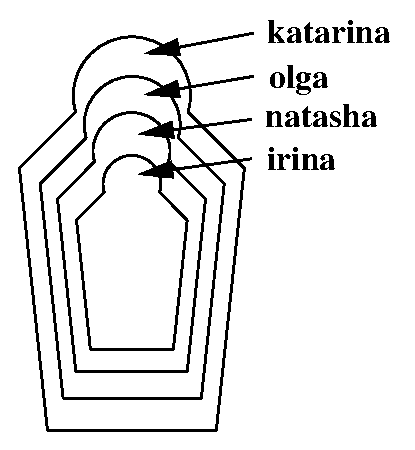
\includegraphics[width=4cm]{dolls.eps}

First, write a knowledge base using the predicate �directlyIn/2� which
encodes which doll is directly contained in which other doll.  Then,
define a recursive predicate �in/2�, that tells us which doll is
(directly or indirectly) contained in which other dolls. For example,
the query �in(katarina,natasha)� should evaluate to true, while
�in(olga, katarina)� should fail.
\end{LPNexercise}


\begin{LPNexercise}{L3.EX3}We have the following knowledge base:
\begin{LPNcodedisplay}
directTrain(saarbruecken,dudweiler).
directTrain(forbach,saarbruecken).
directTrain(freyming,forbach).
directTrain(stAvold,freyming).
directTrain(fahlquemont,stAvold).
directTrain(metz,fahlquemont).
directTrain(nancy,metz).
\end{LPNcodedisplay}

That is, this knowledge base holds facts about towns it is possible to
travel between by taking a \LPNemph{direct} train.  But of course, we can
travel further by chaining together direct train journeys.  Write a
recursive predicate �travelFromTo/2� that tells us when we can
travel by train between two towns.  For example, when given the query
\begin{LPNcodedisplay}
travelFromTo(nancy,saarbruecken).
\end{LPNcodedisplay}
it should reply yes.
\end{LPNexercise}


\begin{LPNexercise}{L3.EX2}Define a predicate �greater_than/2�
that takes two numerals in the notation that we introduced in the text
(that is, 0, succ(0), succ(succ(0)), and so on) as arguments and
decides whether the first one is greater than the second one. For example:
\begin{LPNcodedisplay}
?- greater_than(succ(succ(succ(0))),succ(0)).
yes
?- greater_than(succ(succ(0)),succ(succ(succ(0)))).
no
\end{LPNcodedisplay}
\end{LPNexercise}
\begin{LPNexercise}{L3.EX4}Binary trees
are trees where all internal nodes have exactly two children. The
smallest binary trees consist of only one leaf node. We will represent
leaf nodes as �leaf(Label)�. For instance, �leaf(3)� and �leaf(7)� are
leaf nodes, and therefore small binary trees. Given two binary trees
�B1� and �B2� we can combine them into one binary tree using the
functor �tree/2� as follows: �tree(B1,B2)�.  So, from the leaves
�leaf(1)� and �leaf(2)� we can build the binary tree
�tree(leaf(1),leaf(2))�. And from the binary trees
�tree(leaf(1),leaf(2))� and �leaf(4)� we can build the binary tree
�tree(tree(leaf(1), leaf(2)),leaf(4))�.


Now, define a predicate �swap/2�, which produces the mirror
image of the binary tree that is its first argument. For example:
\begin{LPNcodedisplay}
?- swap(tree(tree(leaf(1), leaf(2)), leaf(4)),T).
T = tree(leaf(4), tree(leaf(2), leaf(1))).
yes
\end{LPNcodedisplay}
\end{LPNexercise}




\section{Practical Session}\label{SEC.L3.PRAXIS}



By now, you should feel more at home with writing and running basic
Prolog programs. In this practical session we first suggest two series
of keyboard exercises which will help you get familiar with recursive
definitions in Prolog, and then give you some programming problems to
solve.

First the keyboard exercises. As recursive programming is so
fundamental to Prolog, it is important that you have a firm grasp of
what it involves. In particular, it is important that you understand
the process of variable instantiation when recursive definitions are
used, and that you understand why the order of goals in rules can make
the difference between termination and non-termination. So:

\begin{enumerate}


\item{} Load �descend1.pl�, turn on �trace�, and pose the query
�descend(anne,emily)�. Count how many steps it takes Prolog to work
out the answer (that is, how many times do you have to hit the return
key).  Now turn �trace� off and pose the query �descend(X,Y)�. How
many answers are there?

\item{}Load �descend2.pl�. This is the variant of �descend1.pl� with
the rule order reversed. Repeat the traces you have
carried out for �descend1.pl�, and compare the results.

\item{}Load �descend3.pl�. This is the variant of �descend2.pl� in
which the goal order within the recursive rule is switched, resulting
in a left recursive rule.  Because of this, even for such simple
queries as �descend(anne,bridget)�, Prolog will not terminate.  Step
through an example, using �trace�, to confirm this.

\item{}Load �descend4.pl�. This is the variant of �descend3.pl�
obtained by switching the rule order.  So �descend4.pl� also contains
a left recursive rule, and does not terminate on all input.  But it
does terminate on some input where �descend3.pl� does not.  Which
extra solutions does it find?

\end{enumerate}

As we said in the text, goal ordering, not rule ordering is
what is truly  procedurally significant.  But with non-terminating programs,
rule ordering changes can have unexpected effects.  Recall the
successor program discussed in the text (let's call it �numeral1.pl�):
\begin{LPNcodedisplay}
numeral(0).
numeral(succ(X)) :- numeral(X).
\end{LPNcodedisplay}
Let's  swap the order of the two clauses, and
call the result �numeral2.pl�:
\begin{LPNcodedisplay}
numeral(succ(X)) :- numeral(X).
numeral(0).
\end{LPNcodedisplay}
Clearly the declarative, or logical, content of this program is
exactly the same as the earlier version. But what are the procedural
differences, if any?

\begin{enumerate}

\item{} Create a file containing �numeral2.pl�, load it, and
investigate what happens if we pose  queries about
\LPNemph{specific} numerals.
For example, suppose we ask:
\begin{LPNcodedisplay}
numeral(succ(succ(succ(0)))).
\end{LPNcodedisplay}
Do �numeral1.pl� and �numeral2.pl� behave in the same way on such
input?

\item{}
Second, look at what happens if we try to \LPNemph{generate} numerals, that
is, suppose we pose the query
\begin{LPNcodedisplay}
numeral(X).
\end{LPNcodedisplay}
Do the programs display identical behaviour?
\end{enumerate}

Here are  some programs for you to try your hand at.
\begin{enumerate}
\item{}Imagine that the following knowledge base describes a maze. The facts
determine which points are connected, that is, from which points you can
get to which other points in one step. Furthermore, imagine that all
paths are one-way streets, so that you can only walk them in one
direction. So, you can get from point 1 to point 2, but not the other
way round.
\begin{LPNcodedisplay}
connected(1,2).
connected(3,4).
connected(5,6).
connected(7,8).
connected(9,10).
connected(12,13).
connected(13,14).
connected(15,16).
connected(17,18).
connected(19,20).
connected(4,1).
connected(6,3).
connected(4,7).
connected(6,11).
connected(14,9).
connected(11,15).
connected(16,12).
connected(14,17).
connected(16,19).
\end{LPNcodedisplay}

Write a predicate �path/2� that tells you from which points
in the maze you can get to which other points when chaining together
connections given in the above knowledge base. Can you get from point
5 to point 10? Which other point can you get to when starting at point
1? And which points can be reached from point 13?
\item{}We are given the following knowledge base of travel information:
\begin{LPNcodedisplay}
byCar(auckland,hamilton).
byCar(hamilton,raglan).
byCar(valmont,saarbruecken).
byCar(valmont,metz).

byTrain(metz,frankfurt).
byTrain(saarbruecken,frankfurt).
byTrain(metz,paris).
byTrain(saarbruecken,paris).

byPlane(frankfurt,bangkok).
byPlane(frankfurt,singapore).
byPlane(paris,losAngeles).
byPlane(bangkok,auckland).
byPlane(singapore,auckland).
byPlane(losAngeles,auckland).
\end{LPNcodedisplay}

Write a predicate �travel/2� which determines whether it is
possible to travel from one place to another by chaining together
car, train, and plane journeys. For example, your program should answer
yes to the query �travel(valmont,raglan)�.

\item{}So, by using �travel/2� to query the above database, you can
find out that it is possible to go from Valmont to Raglan.  If you are
planning such a voyage, that's already something useful to know, but
you would probably prefer to have the precise route from Valmont to
Raglan.  Write a predicate �travel/3� which tells you which route to
take when travelling from one place to another.  For example, the
program should respond
\begin{LPNcodedisplay}
X = go(valmont,metz,
       go(metz,paris,
          go(paris,losAngeles)))
\end{LPNcodedisplay}
to the query
�travel(valmont,losAngeles,X)�.

\item{}Extend the predicate �travel/3� so that it not only tells you
the route to take to get from one place to another, but also
\LPNemph{how} you have to travel. That is, the new program should let
us know, for each stage of the voyage, whether we need to travel by
car, train, or plane.  \end{enumerate}




\chapter{Lists}\label{CHAPTER4}

\Thischapter{145}{

\noindent
This chapter has three main goals:  
  
\begin{enumerate}
\item{}To introduce lists, an important recursive data structure
often used in Prolog programming.
\item{}To define the \texttt{member/2} predicate, a fundamental Prolog tool
for manipulating lists.
\item{} To introduce the idea of recursing down
lists.
\end{enumerate}

}

\section{Lists}\label{SEC.L4.LISTS}



As its name suggests, a list is just a plain old list of  
items. Slightly more precisely, it is a finite sequence of elements.  
Here are some examples of lists in Prolog:  
  
  
\begin{LPNcodedisplay}
[mia, vincent, jules, yolanda]
        
[mia, robber(honey_bunny), X, 2, mia]
        
[]
        
[mia, [vincent, jules], [butch, girlfriend(butch)]]
        
[[], dead(z), [2, [b, c]], [], Z, [2, [b, c]]]
\end{LPNcodedisplay}
  
  
          
We can learn some important things from these examples.  
\begin{enumerate}
\item{}We can specify lists in Prolog by enclosing the
\LPNterm{elements} of the list in square brackets (that is, the symbols
�[� and �]�).  The elements are separated by commas.  For example, the
first list shown above, �[mia, vincent, jules, yolanda]�, is a list with
four elements, namely �mia�, �vincent�, �jules�, and �yolanda�.  The
\LPNterm{length} of a list is the number of elements it has, so our
first example is a list of length four.
\item{}From �[mia,robber(honey_bunny),X,2,mia]�,   
our second example,   
we learn that all sorts of Prolog  
objects can be elements of a list.  The first element of this list is  
�mia�, an atom; the second element is �robber(honey_bunny)�,  
a complex term; the third element is �X�, a variable; the fourth  
element is �2�, a number.  Moreover, we also learn that the same  
item may occur more than once in the same list: for example, the fifth  
element of this list is �mia�, which is same as the first  
element.
\item{}The third example shows that there is a special list,   
        the \LPNterm{empty list}.  The empty list (as its name   
        suggests) is the list that contains no elements.  What is the   
        length of the empty list?  Zero, of course (for the length of a   
        list is the number of members it contains, and the empty list   
        contains nothing).
\item{}The fourth example teaches us something extremely important:   
        lists can contain other lists as elements.  For example, the   
        second element of   
        \begin{LPNcodedisplay}
[mia, [vincent, jules], [butch,girlfriend(butch)]
\end{LPNcodedisplay}
 is   
        �[vincent,jules]�. The   
        third is �[butch,girlfriend(butch)]�. 
          
        What is the length of the fourth list?  The answer is: three.  
If you thought it was five (or indeed, anything else) you're not  
thinking about lists in the right way.  The elements of the list are  
the things between the outermost square brackets separated by commas.  
So this list contains \LPNemph{three} elements: the first element is  
�mia�, the second element is �[vincent, jules]�, and the  
third element is �[butch, girlfriend(butch)]�.
\item{}The last example mixes all these ideas together.  We have   
        here a list which contains the empty list (in fact, it contains it   
        twice), the complex term �dead(z)�, two copies of the list  
        �[2, [b, c]]�, and the variable �Z�.  Note that   
        the third (and the last) elements are lists which themselves   
        contain lists (namely �[b, c]�).
\end{enumerate}


Now for an important point.  Any non-empty list can be thought of as
consisting of two parts: the \LPNterm{head} and the \LPNterm{tail}.  The
head is simply the first item in the list; the tail is everything
else. To put it more precisely, the tail is the list
that remains when we take the first element away; that is,
\LPNemph{the tail of a list is always a list}. For example, the head
of
  
\begin{LPNcodedisplay}
        [mia, vincent, jules, yolanda]
\end{LPNcodedisplay}
is �mia� and the tail is � [vincent, jules, yolanda]�.  
Similarly, the head of  
  \begin{LPNcodedisplay}
[[], dead(z), [2, [b, c]], [], Z, [2, [b, c]]]
\end{LPNcodedisplay}
is �[]�, and the   
tail is �[dead(z), [2,[b,c]],[],Z,[2,[b, c]]]�.  
And what are the head and the tail of the list �[dead(z)]�?  
Well, the head is the first element of the list, which is  
�dead(z)�, and the tail is the list that remains if we take  
the head away, which, in this case, is the empty list �[]�.

What about the empty list? It has neither a head nor a tail.
That is, the empty list has no internal structure; for Prolog,
�[]� is a special, particularly simple, list.  As we shall
learn when we start writing recursive list processing programs, this
fact plays an important role in Prolog programming.

Prolog has a special built-in operator �|� which can be used to
decompose a list into its head and tail. It is important to get to
know how to use �|�, for it is a key tool for writing Prolog list
manipulation programs.

The most obvious use of �|� is to extract information from lists.  We
do this by using �|� together with unification.  For example, to get
hold of the head and tail of �[mia,vincent,� �jules,yolanda]� we can
pose the following query:
  
\begin{LPNcodedisplay}
?- [Head|Tail] = [mia, vincent, jules, yolanda].

Head = mia 
Tail = [vincent,jules,yolanda]
yes 
\end{LPNcodedisplay}
That is, the head of the list has become bound to �Head� and the  
tail of the list has become bound to �Tail�.  Note that there is  
nothing special about �Head� and �Tail�, they are simply  
variables.  We could just as well have posed the query:  
  
  
\begin{LPNcodedisplay}
?- [X|Y] = [mia, vincent, jules, yolanda].

X = mia 
Y = [vincent,jules,yolanda] 
yes
\end{LPNcodedisplay}
  
  
  
As we mentioned above, only non-empty lists have heads and tails.  If   
we try to use �|� to pull �[]� apart, Prolog will fail:  
  
\begin{LPNcodedisplay}
?- [X|Y] = [].

no
\end{LPNcodedisplay}
That is, Prolog treats �[]� as a special list.  This observation   
is extremely  important.  We'll see why later.

Let's look at some other examples.  We can extract the head and tail   
of the following list just as we saw above:  
  
\begin{LPNcodedisplay}
?- [X|Y] = [[], dead(z), [2, [b, c]], [], Z].

X = [] 
Y = [dead(z),[2,[b,c]],[],_7800] 
Z = _7800 
yes
\end{LPNcodedisplay}
That is: the head of the list is bound to �X�, the tail is bound   
to �Y�.  (We also learn that Prolog has bound   
�Z� to the internal variable �_7800�.)

But we  can do a lot more with �|�; it really is a  
flexible tool.  For example, suppose we wanted to know what the first  
\LPNemph{two} elements of the list were, and also the remainder of the  
list after the second element.  Then we'd pose the following query:  
  
\begin{LPNcodedisplay}
?- [X,Y | W] = [[], dead(z), [2, [b, c]], [], Z].

X = [] 
Y = dead(z) 
W = [[2,[b,c]],[],_8327] 
Z = _8327 
yes
\end{LPNcodedisplay}

That is, the head of the list is bound to �X�, the second element is
bound to �Y�, and the remainder of the list after the second element
is bound to �W� (that is, �W� is the list that remains when we take
away the first two elements). So �|� can not only be used to split a
list into its head and its tail, we can also use it to split a list at
any point. To the left of �|� we simply indicate how many elements we
want to take away from the front of the list, and then to right of the
�|� we will get what remains. 

This is a good time to introduce the \LPNterm{anonymous variable}.  
Suppose we were interested in getting hold of the second and fourth  
elements of the list:  
\begin{LPNcodedisplay}
[[], dead(z), [2, [b, c]], [], Z].
\end{LPNcodedisplay}
  
Now, we could find out like this:  
\begin{LPNcodedisplay}
?- [X1,X2,X3,X4 | Tail] = 
            [[], dead(z), [2, [b, c]], [], Z].

X1 = [] 
X2 = dead(z) 
X3 = [2,[b,c]] 
X4 = [] 
Tail = [_8910] 
Z = _8910 
yes
\end{LPNcodedisplay}
  
Ok, we have got the information we wanted: the values we are  
interested in are bound to the variables �X2� and �X4�.  But  
we've got a lot of other information too (namely the values bound to  
�X1�, �X3� and �Tail�). And perhaps we're not  
interested in all this other stuff. If so, it's a bit silly having to  
explicitly introduce variables �X1�, �X3� and �Tail� to  
deal with it.  And in fact, there is a simpler way to obtain \LPNemph{only}  
the information we want: we can pose the following query  
instead:  
  
  
\begin{LPNcodedisplay}
?- [_,X,_,Y|_] = [[], dead(z), [2, [b, c]], [], Z].

X = dead(z) 
Y = [] 
Z = _9593 
yes
\end{LPNcodedisplay}
  
  
The �_� symbol (that is, underscore) is the anonymous variable.  We
use it when we need to use a variable, but we're not interested in
what Prolog instantiates the variable to.  As you can see in the above
example, Prolog didn't bother telling us what �_� was bound to.
Moreover, note that each occurrence of �_� is \LPNemph{independent}:
each is bound to something different. This couldn't happen with an
ordinary variable of course, but then the anonymous variable isn't
meant to be ordinary. It's simply a way of telling Prolog to bind
something to a given position, completely independently of any other
bindings.

Let's look at one last example. The third element of our working  
example is a list (namely �[2, [b, c]]�).  Suppose we  
wanted to extract the tail of this internal list, and that we are not  
interested in any other information.  How could we do this?  As  
follows:  
  
\begin{LPNcodedisplay}
?- [_,_,[_|X]|_] = 
      [[], dead(z), [2, [b, c]], [], Z, [2, [b, c]]].

X = [[b,c]] 
Z = _10087 
yes
\end{LPNcodedisplay}




\section{Member}\label{SEC.L4.MEMBER}

It's time to look at our first example of a recursive Prolog program
for manipulating lists.  One of the most basic things we would like to
know is whether something is an element of a list or not.  So let's
write a program that, when given as inputs an arbitrary object
\LPNemph{X} and a list \LPNemph{L}, tells us whether or not
\LPNemph{X} belongs to \LPNemph{L}.  The program that does this is
usually called \LPNterm{member}\index{PROLOG
member/2@\texttt{member/2}}, and it is the simplest example of a
Prolog program that exploits the recursive structure of lists.  Here
it is:
  
  
\begin{LPNcodedisplay}
member(X,[X|T]).
member(X,[H|T]) :- member(X,T).
\end{LPNcodedisplay}
  
  
That's all there is to it: one fact (namely �member(X,[X|T])�)  
and one rule (namely �member(X,[H|T]) :- member(X,T)�). But note  
that the rule is recursive (after all, the functor �member�  
occurs in both the rule's head and body) and it is this that explains  
why such a short program is all that is required.  
Let's take a closer look.

We'll start by reading the program declaratively. And read this way,  
it is obviously sensible.  The first clause (the fact) simply says: an  
object �X� is a member of a list if it is the head of that list.  
Note that we used the built-in �|� operator to state this (simple  
but important) principle about lists.

 What about the second clause, the recursive rule?  This says: an  
object �X� is member of a list if it is a member of the tail of  
the list.  Again, note that we used the �|� operator to state  
this principle.

Now, clearly this definition makes good declarative sense.  But does  
this program actually \LPNemph{do} what it is supposed to do?  That is,  
will it really tell us whether an object �X� belongs to a list  
�L�? And if so, how exactly does it do this?  To answer such  
questions, we need to think about its procedural meaning.  Let's work  
our way through a few examples.

Suppose we posed the following query:  
  
\begin{LPNcodedisplay}
?- member(yolanda,[yolanda,trudy,vincent,jules]).
\end{LPNcodedisplay}
Prolog will immediately answer yes.  Why?  Because it can unify  
�yolanda� with both occurrences of �X� in the first clause  
(the fact) in the definition of �member/2�, so it succeeds  
immediately.

Next consider the following query:  
  
\begin{LPNcodedisplay}
?- member(vincent,[yolanda,trudy,vincent,jules]).
\end{LPNcodedisplay}
Now the first rule won't help (�vincent� and �yolanda� are  
distinct atoms) so Prolog goes to the second clause, the recursive  
rule. This gives Prolog a new goal: it now has to see if  
  
\begin{LPNcodedisplay}
member(vincent,[trudy,vincent,jules]).
\end{LPNcodedisplay}
Once again the first clause won't help, so Prolog goes (again) to  
the recursive rule. This gives it a new goal, namely  
  
\begin{LPNcodedisplay}
member(vincent,[vincent,jules]).
\end{LPNcodedisplay}
This time, the first clause does help, and the query succeeds.

So far so good, but we need to ask an important question.  What  
happens when we pose a query that \LPNemph{fails}?  For example, what  
happens if we pose the query  
  
\begin{LPNcodedisplay}
member(zed,[yolanda,trudy,vincent,jules]).
\end{LPNcodedisplay}
  
  
Now, this should obviously fail (after all, �zed� is not on the  
list).  So how does Prolog handle this?  In particular, how can we be  
sure that Prolog really will \LPNemph{stop}, and say \LPNemph{no}, instead  
going into an endless recursive loop?

Let's think this through systematically.  Once again, the first clause  
cannot help, so Prolog uses the recursive rule, which gives it a new  
goal  
  
\begin{LPNcodedisplay}
member(zed,[trudy,vincent,jules]).
\end{LPNcodedisplay}
Again, the first clause doesn't help, so Prolog reuses the recursive  
rule and tries to show that  
  
\begin{LPNcodedisplay}
member(zed,[vincent,jules]).
\end{LPNcodedisplay}
Similarly, the first rule doesn't help, so Prolog reuses the second  
rule yet again and   
tries the goal  
\begin{LPNcodedisplay}
member(zed,[jules]).
\end{LPNcodedisplay}
Again the first clause doesn't help, so Prolog uses the second rule,  
which gives it the goal  
  
\begin{LPNcodedisplay}
member(zed,[])
\end{LPNcodedisplay}
And \LPNemph{this} is where things get interesting.  Obviously the
first clause can't help here.  But note: \LPNemph{the recursive rule
can't do anything more either}.  Why not? Simple: the recursive rule
relies on splitting the list into a head and a tail, but as we have
already seen, the empty list \LPNemph{can't} be split up in this way.
So the recursive rule cannot be applied either, and Prolog stops
searching for more solutions and announces no.  That is, it tells us
that �zed� does not belong to the list, which is just what it ought to
do.

We could summarise the �member/2� predicate as follows.  It  
is a recursive predicate, which systematically searches down the  
length of the list for the required item.  It does this by stepwise  
breaking down the list into smaller lists, and looking at the first  
item of each smaller list.  This mechanism that drives this  
search is recursion, and the reason that this recursion is safe (that  
is, the reason it does not go on forever) is that at the end of the  
line Prolog has to ask a question about the empty list.  The empty  
list \LPNemph{cannot} be broken down into smaller parts, and this allows a  
way out of the recursion.

Well, we've now seen why �member/2� works, but in fact it's  
far more useful than the previous example might suggest.  Up till now  
we've only been using it to answer yes/no questions.  But we can also  
pose questions containing variables.  For example, we can have the  
following dialog with Prolog:  
  
  
\begin{LPNcodedisplay}
member(X,[yolanda,trudy,vincent,jules]).

X = yolanda ;

X = trudy ;

X = vincent ;

X = jules ;

no
\end{LPNcodedisplay}
  
  
That is, Prolog has told us what every member of a list is.  This is
an extremely common use of �member/2�. In effect, by using the
variable we are saying to Prolog: ``Quick! Give me some element of the
list!''. In many applications we need to be able to extract members of
a list, and this is the way it is typically done.



One final remark.  The way we defined �member/2� above is  
certainly correct, but in one respect it is a little messy.

Think about it. The first clause is there to deal with the head of the  
list. But although the tail is irrelevant to the first clause, we  
named the tail using the variable �T�. Similarly,  
the recursive rule is there to deal with the tail of the list.  But  
although the head is irrelevant here, we named it  
using the variable  �H�. These unnecessary variable  
names are distracting: it's better to write predicates in a way that  
focuses attention on what is really important in each clause, and the  
anonymous variable gives us a nice way of doing this. That is, we  can rewrite  
�member/2� as follows:  
\begin{LPNcodedisplay}
member(X,[X|_]).
member(X,[_|T]) :- member(X,T).
\end{LPNcodedisplay}
  
This version is exactly the same, both declaratively and procedurally.  
But it's just that little bit clearer: when you read it, you are  
forced to concentrate on what is essential.  


\section{Recursing down Lists}\label{SEC.L4.RDAL}

The �member/2� predicate works by recursively working its way down a
list, doing something to the head, and then recursively doing the same
thing to the tail. Recursing down a list (or indeed, several lists) in
this way is extremely common in Prolog; so common, in fact, that it is
important that you really master the technique. So let's look at another
example.

When working with lists, we often want to compare one list  
with another, or to copy bits of one list into another, or to  
translate the contents of one list into another, or something similar.  
Here's an example. Let's suppose we need a predicate  
�a2b/2� that takes two lists as arguments, and succeeds if  
the first argument is a list of �a�s, and the second argument is  
a list of �b�s of exactly the same length.  For example, if we  
pose the following query  
\begin{LPNcodedisplay}
a2b([a,a,a,a],[b,b,b,b]).
\end{LPNcodedisplay}
we want Prolog to say yes. On the other hand, if we pose the query  
\begin{LPNcodedisplay}
a2b([a,a,a,a],[b,b,b]).
\end{LPNcodedisplay}
or the query  
\begin{LPNcodedisplay}
a2b([a,c,a,a],[b,b,5,4]).
\end{LPNcodedisplay}
we want Prolog to say no.

When faced with such tasks, often the best way to set about solving
them is to start by thinking about the simplest possible case. Now,
when working with lists, thinking about the simplest case often means
thinking about the empty list, and it certainly means this here.
After all: what is the shortest possible list of �a�s?  It's the empty
list. Why? Because it contains no �a�s at all. And what is the
shortest possible list of �b�s? Again, the empty list: no �b�s
whatsoever in that.  So the most basic information our definition
needs to contain is
\begin{LPNcodedisplay}
a2b([],[]).
\end{LPNcodedisplay}
This records the obvious fact that the empty list contains exactly as  
many �a�s as �b�s. But although obvious, this fact turns out  
to play an important role in our program, as we shall see.

 So far so good: but how do we proceed? Here's the idea: for longer  
lists, \LPNemph{think recursively}. So: when should �a2b/2�  
decide that two non-empty lists are a list of �a�s and a list of  
�b�s of exactly the same length? Simple: when the head of the  
first list is an �a�, and the head of the second list is a  
�b�, and �a2b/2� decides that the two tails are lists  
of �a�s and �b�s of exactly the same length!  This  
immediately gives us the following rule:  
\begin{LPNcodedisplay}
a2b([a|Ta],[b|Tb]) :- a2b(Ta,Tb).
\end{LPNcodedisplay}
This says: the �a2b/2� predicate should succeed if its  
first argument is a list with head �a�, its second argument is a  
list with head �b�, and �a2b/2� succeeds on the two  
tails.

Now, this definition make good sense declaratively. It is a simple and  
natural recursive predicate, the base clause dealing with the empty  
list, the recursive clause dealing with non-empty lists.  But how does  
it work in practice? That is, what is its procedural meaning?  For  
example, if we pose the query  
\begin{LPNcodedisplay}
a2b([a,a,a],[b,b,b]).
\end{LPNcodedisplay}
Prolog will say yes, which is what we want --- but \LPNemph{why} exactly does  
this happen?

Let's work the example through. In this query, neither list is empty,  
so the fact does not help. Thus Prolog goes on to try the recursive  
rule. Now, the query does match the rule (after all, the head of the  
first list is �a� and the head of the second is �b�) so  
Prolog now has a new goal, namely  
\begin{LPNcodedisplay}
a2b([a,a],[b,b]).
\end{LPNcodedisplay}
Once again, the fact does not help with this, but the recursive rule  
can be used again, leading to the following goal:  
\begin{LPNcodedisplay}
a2b([a],[b]).
\end{LPNcodedisplay}
Yet again the fact does not help, but the recursive rule does, so we  
get the following goal:  
\begin{LPNcodedisplay}
a2b([],[]).
\end{LPNcodedisplay}
At last we can use the fact: this tells us that, yes, we really do  
have two lists here that contain exactly the same number of �a�s  
and �b�s (namely, none at all). And because this goal succeeds,  
this means that the goal  
\begin{LPNcodedisplay}
a2b([a],[b]).
\end{LPNcodedisplay}
succeeds too. This in turn means that the goal  
\begin{LPNcodedisplay}
a2b([a,a],[b,b]).
\end{LPNcodedisplay}
succeeds, and thus that the original goal  
\begin{LPNcodedisplay}
a2b([a,a,a],[b,b,b]).
\end{LPNcodedisplay}
is satisfied.

We could summarise this process as follows.  Prolog started with two
lists. It peeled the head off each of them, and checked that they were
an �a� and a �b�, respectively, as required. It then recursively
analysed the tails of both lists. That is, it worked its way down both
tails simultaneously, checking that at each stage the tails were
headed by an �a� and a �b�.  Why did the process stop?  Because at
each recursive step we had to work with shorter lists (namely the
tails of the lists examined at the previous step) and eventually we
ended up with empty lists.  At this point, our rather trivial looking
fact was able to play a vital role: it said yes. This halted the
recursion, and ensured that the original query succeeded.

It's is also important to think about what  happens with queries  
that \LPNemph{fail}. For example, if we pose the query  
\begin{LPNcodedisplay}
a2b([a,a,a,a],[b,b,b]).
\end{LPNcodedisplay}
Prolog will correctly say no. Why? because after carrying out the
peel-off-the-head-and-recursively-examine-the-tail process three
times, it will be left with the query
\begin{LPNcodedisplay}
a2b([a],[]).
\end{LPNcodedisplay}
But this goal cannot be satisfied.   
And if we pose the query  
\begin{LPNcodedisplay}
a2b([a,c,a,a],[b,b,5,4]).
\end{LPNcodedisplay}
after carrying out the
peel-off-the-head-and-recursively-examine-the-tail process once,
Prolog will have the goal
\begin{LPNcodedisplay}
a2b([c,a,a],[b,5,4]).
\end{LPNcodedisplay}
and again, this cannot be satisfied.

Well, that's how �a2b/2� works in simple cases, but we  
haven't exhausted its possibilities yet. As always with Prolog, it's a  
good idea to investigate what happens when variables as used as  
input. And with �a2b/2� something interesting happens: it  
acts as a translator, translating lists of �a�s to lists of  
�b�s, and vice versa.  For example the query  
\begin{LPNcodedisplay}
a2b([a,a,a,a],X).
\end{LPNcodedisplay}
yields the response  
\begin{LPNcodedisplay}
X = [b,b,b,b].
\end{LPNcodedisplay}
That is, the list of �a�s has been translated to a list of   
�b�s. Similarly, by using a variable in the first argument  
position, we can use it to translate lists of �b�s  
to lists of �a�s:  
\begin{LPNcodedisplay}
a2b(X,[b,b,b,b]).

X = [a,a,a,a]
\end{LPNcodedisplay}
  
And of course, we can use variables in both argument positions:  
\begin{LPNcodedisplay}
a2b(X,Y).
\end{LPNcodedisplay}
Can you work out what happens in this case?

To sum up: �a2b/2� is an extremely simple example of a  
program that works by recursing its way down a pair of lists. But  
don't be fooled by its simplicity: the kind of programming it  
illustrates is fundamental to Prolog.  Both its declarative form (a  
base clause dealing with the empty list, a recursive clause dealing  
with non-empty lists) and the procedural idea it trades on (do  
something to the heads, and then recursively do the same thing to the  
tails) come up again and again in Prolog programming. In fact, in the  
course of your Prolog career, you'll find that you'll write what is  
essentially the �a2b/2� predicate, or a more complex  
variant of it, many times over in many different guises.

\section{Exercises}\label{SEC.L4.EXERCISES}

\begin{LPNexercise}{L4.EX1}How does Prolog respond to the following queries?  
\begin{enumerate}
\item{}�[a,b,c,d] = [a,[b,c,d]].�
\item{}�[a,b,c,d] = [a|[b,c,d]].�
\item{}�[a,b,c,d] = [a,b,[c,d]].�
\item{}�[a,b,c,d] = [a,b|[c,d]].�
\item{}�[a,b,c,d] = [a,b,c,[d]].�
\item{}�[a,b,c,d] = [a,b,c|[d]].�
\item{}�[a,b,c,d] = [a,b,c,d,[]].�
\item{}�[a,b,c,d] = [a,b,c,d|[]].�
\item{}�[] = _.�
\item{}�[] = [_].�
\item{}�[] = [_|[]].�
\end{enumerate}
\end{LPNexercise}
\begin{LPNexercise}{L4.EX1.2}Which of the following are syntactically correct lists? If the representation is correct, how many elements does the list have?  

\begin{enumerate}
\item{}�[1|[2,3,4]]�
\item{}�[1,2,3|[]]�
\item{}�[1|2,3,4]�


\item{}�[1|[2|[3|[4]]]]�
\item{}�[1,2,3,4|[]]�
\item{}�[[]|[]]�
\item{}�[[1,2]|4]�
\item{}�[[1,2],[3,4]|[5,6,7]]�


\end{enumerate}
\end{LPNexercise}


\begin{LPNexercise}{L6.EX3a}
Write a predicate �second(X,List)� which checks  
whether �X� is the second element of �List�.
\end{LPNexercise}


\begin{LPNexercise}{L6.EX3b}
Write a predicate �swap12(List1,List2)� which checks  
whether �List1� is identical to �List2�, except that the  
first two elements are exchanged.
\end{LPNexercise}


\begin{LPNexercise}{L4.EX2}Suppose we are given a knowledge base with the following facts:  
  
\begin{LPNcodedisplay}
tran(eins,one).
tran(zwei,two).
tran(drei,three).
tran(vier,four).
tran(fuenf,five).
tran(sechs,six).
tran(sieben,seven).
tran(acht,eight).
tran(neun,nine).
\end{LPNcodedisplay}
  
  
         
Write a predicate �listtran(G,E)� which translates a list of   
German number words to the corresponding list of English number words.    
For example:  
\begin{LPNcodedisplay}
listtran([eins,neun,zwei],X).
\end{LPNcodedisplay}
should give:  
\begin{LPNcodedisplay}
X = [one,nine,two].
\end{LPNcodedisplay}

Your program should also work in the other direction. For example, if   
you give it the query  
\begin{LPNcodedisplay}
listtran(X,[one,seven,six,two]).
\end{LPNcodedisplay}
it should return:  
\begin{LPNcodedisplay}
X = [eins,sieben,sechs,zwei].
\end{LPNcodedisplay}
  
  
(Hint: to answer this question, first ask yourself ``How do I  
translate the \LPNemph{empty} list of number words?''.  That's the base  
case.  For non-empty lists, first translate the head of the list, then  
use recursion to translate the tail.)
\end{LPNexercise}


\begin{LPNexercise}{L4.EX3}Write a predicate �twice(In,Out)� 
whose left argument is a list,   
and whose right argument is a list consisting of every element in the
left list written twice.  For example, the query
\begin{LPNcodedisplay}
twice([a,4,buggle],X).
\end{LPNcodedisplay}
should return  
\begin{LPNcodedisplay}
X = [a,a,4,4,buggle,buggle]).
\end{LPNcodedisplay}
And the query  
\begin{LPNcodedisplay}
twice([1,2,1,1],X).
\end{LPNcodedisplay}
should return  
\begin{LPNcodedisplay}
X = [1,1,2,2,1,1,1,1].
\end{LPNcodedisplay}
  
(Hint: to answer this question, first ask yourself ``What should happen  
when the first argument is the \LPNemph{empty} list?''.  That's the base case.  
For non-empty lists, think about what you should do with the head, and  
use recursion to handle the tail.)
\end{LPNexercise}


\begin{LPNexercise}{L4.EX4}Draw the search trees for the following three queries:  
  
\begin{LPNcodedisplay}
?- member(a,[c,b,a,y]).

?- member(x,[a,b,c]).

?- member(X,[a,b,c]).

\end{LPNcodedisplay}
(Search trees were introduced in Chapter~\ref{CHAPTER2}.)
\end{LPNexercise}


\section{Practical Session}\label{SEC.L4.PRAXIS}



The purpose of Practical Session 4 is to help you get familiar with  
the idea of recursing down lists.  We first suggest some traces for  
you to carry out, and then some programming exercises.

First, systematically carry out a number of traces on  
�a2b/2� to make sure you fully understand how it   
works. In particular:  
  
\begin{enumerate}
\item{}Trace some examples, not involving variables, that succeed. For
example, trace the query �a2b([a,a,a,a],[b,b,b,b])� and relate the
output to the discussion in the text.
\item{}Trace some simple examples that fail. Try  
examples involving  lists of different lengths  
(such as �a2b([a,a,a,a],[b,b,b])�) and  
examples involving  symbols other than �a� and �b�  
(such as �a2b([a,c,a,a],[b,b,5,4])�). 
\item{}Trace some examples involving variables. For example, try  
tracing �a2b([a,a,a,a],X)� and �a2b(X,[b,b,b,b])�.
\item{}Make sure you understand what happens when  
both arguments in the query are variables. For example, carry  
out a trace on the query �a2b(X,Y)�.
\item{}Carry out a series of similar traces involving  
�member/2�. That is, carry out traces involving simple queries that  
succeed (such as �member(a,[1,2,a,b])�), simple queries that fail  
(such as �member(z,[1,2,a,b])�), and queries involving variables  
(such as �member(X,[1,2,a,b])�).  In all cases, make sure that  
you understand why the recursion halts.
\end{enumerate}


Having done this, try the following.  
  
\begin{enumerate}
\item{}Write a 3-place predicate �combine1� which takes three  
lists as arguments and combines the elements of the first two lists  
into the third as follows:  
\begin{LPNcodedisplay}
?- combine1([a,b,c],[1,2,3],X).

X = [a,1,b,2,c,3]

?- combine1([f,b,yip,yup],[glu,gla,gli,glo],Result).

Result = [f,glu,b,gla,yip,gli,yup,glo]
\end{LPNcodedisplay}

\item{}Now write a 3-place predicate �combine2� which takes three  
lists as arguments and combines the elements of the first two lists  
into the third as follows:  
\begin{LPNcodedisplay}
?- combine2([a,b,c],[1,2,3],X).

X = [[a,1],[b,2],[c,3]]

?- combine2([f,b,yip,yup],[glu,gla,gli,glo],Result).

Result = [[f,glu],[b,gla],[yip,gli],[yup,glo]]
\end{LPNcodedisplay}

\item{}Finally, write a 3-place predicate �combine3� which takes  
three lists as arguments and combines the elements of the first two lists  
into the third as follows:  
\begin{LPNcodedisplay}
?- combine3([a,b,c],[1,2,3],X).

X = [j(a,1),j(b,2),j(c,3)]

?- combine3([f,b,yip,yup],[glu,gla,gli,glo],R).

R = [j(f,glu),j(b,gla),j(yip,gli),j(yup,glo)]
\end{LPNcodedisplay}

\end{enumerate}
  
All three programs are pretty much the same as �a2b/2� (though they
manipulate three lists, not two).  That is, all three can be written
by recursing down the lists, doing something to the heads, and then
recursively doing the same thing to the tails.  Indeed, once you have
written �combine1�, you just need to change what you do to the heads
to get �combine2� and �combine3�.




\chapter{Arithmetic}\label{CHAPTER5}

\Thischapter{120}{

\noindent
This chapter has two main goals:

\begin{enumerate}
\item{}To introduce Prolog's built-in abilities for performing
       arithmetic.
\item{}To apply them to simple list processing problems, using
       accumulators.
\end{enumerate}

}

\section{Arithmetic in Prolog}\label{SEC.L5.ARITHMETIC}



Prolog provides a number of basic arithmetic tools for manipulating
integers (that is, numbers of the form ...-3, -2, -1, 0, 1, 2, 3,
4...).  Most Prolog implementation also provide tools for handling
real numbers (or floating point numbers) such as 1.53 or $6.35\times
10^{5}$, but we're not going to discuss these, for they are not
particularly useful for the symbolic processing tasks discussed in
this book.  Integers, on the other hand, are useful in connection with
symbolic tasks (we use them to state the length of lists, for example)
so it is important to understand how to work with them.  We'll start
by looking at how Prolog handles the four basic operations of
addition, multiplication, subtraction, and division.

\begin{center}\begin{tabular}{ll}
Arithmetic examples & Prolog Notation\\
$6+2=8$&�8 is 6+2.�\\
$6*2=12$&�12 is 6*2.�\\
$6-2=4$&�4 is 6-2.�\\
$6-8=-2$&�-2 is 6-8.�\\
$6\div 2=3$&�3 is 6/2.�\\
$7\div 2=3$&�3 is 7/2.�\\
1 is the remainder when 7 is divided by 2&�1 is mod(7,2).�
\end{tabular}\end{center}
Note that as we are working with integers, division gives us back an
integer answer.  Thus $7\div 2$ gives 3 as an answer,  leaving
remainder 1.

Posing the following queries yields the following responses\index{PROLOG is/2@\texttt{is/2}}:

\begin{LPNcodedisplay}
?- 8 is 6+2.
yes

?- 12 is 6*2.
yes

?- -2 is 6-8.
yes

?- 3 is 6/2.
yes

?- 1 is mod(7,2).
yes
\end{LPNcodedisplay}


More importantly, we can work out the answers to arithmetic questions
by using variables.  For example:

\begin{LPNcodedisplay}
?- X is 6+2.

X = 8

?- X is 6*2.

X = 12

?- R is mod(7,2).

R = 1
\end{LPNcodedisplay}

Moreover, we can use arithmetic operations when we define predicates.
Here's a simple example.  Let's define a predicate
�add_3_and_double/2� whose arguments are both integers.  This
predicate takes its first argument, adds three to it, doubles the
result, and returns the number obtained as the second argument.  We
define this predicate as follows:
\begin{LPNcodedisplay}
add_3_and_double(X,Y) :- Y is (X+3)*2.
\end{LPNcodedisplay}
And indeed, this works:
\begin{LPNcodedisplay}
?- add_3_and_double(1,X).

X = 8

?- add_3_and_double(2,X).

X = 10
\end{LPNcodedisplay}


One other thing.  Prolog understands the usual conventions we use for
disambiguating arithmetical expressions.  For example, when we write
$3+2\times 4$ we mean $3+(2\times 4)$ and not $(3+2)\times 4$, and
Prolog knows this convention:
\begin{LPNcodedisplay}
?- X is 3+2*4.

X = 11
\end{LPNcodedisplay}





\section{A Closer Look}\label{SEC.L5.LOOK}

That's the basics, but we need to know more.  The most important to
grasp is this: +, *, -, $\div$ and �mod� do \LPNemph{not} carry out
any arithmetic.  In fact, expressions such as �3+2�, �3-2� and �3*2�
are simply terms.  The functors of these terms are �+�, �-� and �*�
respectively, and the arguments are �3� and �2�.  Apart from the fact
that the functors go between their arguments (instead of in front of
them) these are ordinary Prolog terms, and unless we do something
special, Prolog will not actually do any arithmetic.  In
particular, if we pose the query
\begin{LPNcodedisplay}
?- X = 3+2
\end{LPNcodedisplay}
we don't get back the answer �X=5�.
Instead we get back
\begin{LPNcodedisplay}
X = 3+2
yes
\end{LPNcodedisplay}
That is, Prolog has simply unified the variable �X� to the complex
term �3+2�.  It has \LPNemph{not} carried out any arithmetic.  It has
simply done what it usually does when \texttt{=/2} is used: performed
unification.

Similarly,
if we pose the query
\begin{LPNcodedisplay}
?- 3+2*5 = X
\end{LPNcodedisplay}
we get the response
\begin{LPNcodedisplay}
X = 3+2*5
yes
\end{LPNcodedisplay}
Again, Prolog has simply bound the variable �X� to the complex
term �3+2*5�.  It did not evaluate this expression to 13.

To force Prolog to actually evaluate arithmetic expressions we have to
use
        \begin{LPNcodedisplay}
is
\end{LPNcodedisplay}
just as we did in our  earlier examples.  In fact, �is� does
something very special: it sends a signal to Prolog that says ``Hey!
Don't treat this expression as an ordinary complex term!  Call up
your built-in arithmetic capabilities and carry out the calculations!''

In short, �is� forces Prolog to act in an unusual way.  Normally
Prolog is quite happy just unifying variables to structures: that's
its job, after all.  Arithmetic is something extra that has been
bolted on to the basic Prolog engine because it is useful.
Unsurprisingly, there are some restrictions on this extra ability, and
we need to know what they are.

For a start, the arithmetic expressions to be evaluated must be on
the right hand side of �is�.  In our earlier examples we carefully
posed the query
\begin{LPNcodedisplay}
?- X is 6+2.

X = 8
\end{LPNcodedisplay}
which is the right way to do it. If instead we
had asked
\begin{LPNcodedisplay}
6+2 is X.
\end{LPNcodedisplay}
we would have got a message saying �instantiation_error�,
or something similar.

Moreover, although we are free to use variables on the right hand side
of �is�, when we actually carry out evaluation, the variable must
already have been instantiated to a variable-free arithmetic
expression.  If the variable is uninstantiated, or if it is
instantiated to something other than an integer, we will get some sort
of �instantiation_error� message.  This is because arithmetic isn't
performed using Prolog's usual unification and knowledge base search
mechanisms: it's done by calling up a special black box which knows
about integer arithmetic.  If we hand the black box the wrong kind of
data, it's going to complain.

Here's an example. Recall our ``add 3 and double it''
predicate.
\begin{LPNcodedisplay}
add_3_and_double(X,Y) :- Y is (X+3)*2.
\end{LPNcodedisplay}
When we described this predicate, we carefully said that it added 3 to
its first argument, doubled the result, and returned the answer in its
second argument.  For example, �add_3_and_double(3,X)� returns
�X = 12�.  We didn't say anything about using this predicate in
the reverse direction.  For example, we might hope that posing the
query
\begin{LPNcodedisplay}
?- add_3_and_double(X,12).
\end{LPNcodedisplay}
would return the answer �X=3�.   But it doesn't. Instead we
get the �instantiation_error� message.  Why?  Well, when we pose
the query this way round, we are asking Prolog to evaluate
�12 is (X+3)*2�, which it \LPNemph{can't} do as �X�
is not instantiated.

Two final remarks.  As we've already mentioned, for Prolog �3 + 2�
is just a term.  In fact, for Prolog, it really \LPNemph{is} the term
\LPNemph{+(3,2)}.  The expression �3 + 2� is just a user-friendly
notation that's nicer for us to use.  This means that, if you
want to, you can give Prolog queries like
\begin{LPNcodedisplay}
X is +(3,2)
\end{LPNcodedisplay}
and Prolog will correctly reply
\begin{LPNcodedisplay}
X = 5
\end{LPNcodedisplay}
Actually, you can even given Prolog the query
\begin{LPNcodedisplay}
?- is(X,+(3,2))
\end{LPNcodedisplay}
and Prolog will respond
\begin{LPNcodedisplay}
X = 5
\end{LPNcodedisplay}
This is because, for Prolog, the expression �X is +(3,2)� really is
the term �is(X,+(3,2))�.  The expression �X is +(3,2)� is just
user-friendly notation.  Underneath, as always, Prolog is just working
away with terms.

Summing up, arithmetic in Prolog is easy to use.  Pretty much all you
have to remember is to use �is� to force evaluation, that stuff to be
evaluated must go to the right of �is�, and to take care that any
variables are correctly instantiated.  But there is a deeper point
that is worth reflecting on: bolting on the extra capability to do
arithmetic in this way has further widened the gap between the
procedural and declarative meanings of Prolog programs.





\section{Arithmetic and Lists}\label{SEC.L5.ARITHMETIC-AND-LISTS}

Probably the most important use of arithmetic in this book is to tell
us useful facts about data-structures, such as lists.  For example, it
can be useful to know how long a list is.  We'll give some examples of
using lists together with arithmetic capabilities.

How long is a list? Here's a recursive definition.
\begin{enumerate}
\item{}The empty list has length zero.
\item{}A non-empty list has length
         1 + \LPNemph{len}(T), where \LPNemph{len}(T) is the length of its
        tail.
\end{enumerate}


This definition is practically a Prolog program already.  Here's the
code we need:
\begin{LPNcodedisplay}
len([],0).
len([_|T],N) :- len(T,X), N is X+1.
\end{LPNcodedisplay}

This predicate works in the expected way.
For example:
\begin{LPNcodedisplay}
?- len([a,b,c,d,e,[a,b],g],X).

X = 7
\end{LPNcodedisplay}

\clearpage
Now, this is quite a good program: it's easy to understand and
efficient.  But there is another method of finding the length of a
list.  We'll now look at this alternative, because it introduces the
idea of \LPNterm{accumu\-lators}. If you're used to other programming
languages, you're probably used to the idea of using variables to hold
intermediate results.  An accumulator is the Prolog analog of this
idea.


Here's how to use an accumulator to calculate the length of a list.
We shall define a predicate �accLen�/3 which takes the following
arguments.
\begin{LPNcodedisplay}
accLen(List,Acc,Length)
\end{LPNcodedisplay}
Here �List� is the list whose length we want to find, and �Length� is
its length (an integer).  What about �Acc�?  This is the accumulator
we will use to keep track of intermediate values for length (so it
will also be an integer).  Here's what we do.  When we call this
predicate, we are going to give �Acc� an initial value of �0�.  We
then recursively work our way down the list, adding �1� to �Acc� each
time we find a head element, until we reach the empty list.  When we
reach the empty list, �Acc� will contain the length of the list.
Here's the code:
\begin{LPNcodedisplay}
accLen([_|T],A,L) :-  Anew is A+1, accLen(T,Anew,L).
accLen([],A,A).
\end{LPNcodedisplay}

The base case of the definition, unifies the second and third
arguments.  Why?  Because this trivial unification is a nice way of
making sure that the result, that is, the length of the list, is
returned. When we reach the end of the list, the accumulator (the
second variable) contains the length of the list.  So we give this
value (via unification) to the length variable (the third variable).
Here's an example trace. You can clearly see how the length variable
gets its value at the bottom of the recursion and passes it upwards as
Prolog is coming out of the recursion.
\begin{LPNcodedisplay}
?- accLen([a,b,c],0,L).
   Call: (6) accLen([a, b, c], 0, _G449) ?
   Call: (7) _G518 is 0+1 ?
   Exit: (7) 1 is 0+1 ?
   Call: (7) accLen([b, c], 1, _G449) ?
   Call: (8) _G521 is 1+1 ?
   Exit: (8) 2 is 1+1 ?
   Call: (8) accLen([c], 2, _G449) ?
   Call: (9) _G524 is 2+1 ?
   Exit: (9) 3 is 2+1 ?
   Call: (9) accLen([], 3, _G449) ?
   Exit: (9) accLen([], 3, 3) ?
   Exit: (8) accLen([c], 2, 3) ?
   Exit: (7) accLen([b, c], 1, 3) ?
   Exit: (6) accLen([a, b, c], 0, 3) ?
\end{LPNcodedisplay}

As a final step, we'll define a predicate which calls �accLen�
for us, and gives it the initial value of 0:
\begin{LPNcodedisplay}
leng(List,Length) :- accLen(List,0,Length).
\end{LPNcodedisplay}
So now we can pose queries like this:
\begin{LPNcodedisplay}
?- leng([a,b,c,d,e,[a,b],g],X).
\end{LPNcodedisplay}


Accumulators are extremely common in Prolog programs.  (We'll see
another accumulator based program in this chapter, and some more in
later chapters.) But why is this? In what way is �accLen� better than
�len�? After all, it looks more difficult. The answer is that �accLen�
is \LPNterm{tail recursive} while �len� is not. In tail recursive
programs, the result is fully calculated once we reached the bottom of
the recursion and just has to be passed up. In recursive programs
which are not tail recursive, there are goals at other levels of
recursion which have to wait for the answer from a lower level of
recursion before they can be evaluated. To understand this, compare
the traces for the queries �accLen([a,b,c],0,L)� (see above) and
�len([a,b,c],0,L)� (given below). In the first case the result is
built while going into the recursion --- once the bottom is reached at
�accLen([],3,_G449)�, the result is there and only has to be passed
up. In the second case the result is built while coming out of the
recursion; the result of �len([b,c], _G481)�, for instance, is only
computed after the recursive call of �len� has been completed and the
result of �len([c],_G489)� is known. In short, tail recursive programs
have less bookkeeping overhead, and this makes them more efficient.

\begin{LPNcodedisplay}
?- len([a,b,c],L).
   Call: (6) len([a, b, c], _G418) ?
   Call: (7) len([b, c], _G481) ?
   Call: (8) len([c], _G486) ?
   Call: (9) len([], _G489) ?
   Exit: (9) len([], 0) ?
   Call: (9) _G486 is 0+1 ?
   Exit: (9) 1 is 0+1 ?
   Exit: (8) len([c], 1) ?
   Call: (8) _G481 is 1+1 ?
   Exit: (8) 2 is 1+1 ?
   Exit: (7) len([b, c], 2) ?
   Call: (7) _G418 is 2+1 ?
   Exit: (7) 3 is 2+1 ?
   Exit: (6) len([a, b, c], 3) ?
\end{LPNcodedisplay}


\section{Comparing Integers}\label{SEC.L5.COMPARING-INTEGERS}



Some Prolog arithmetic predicates actually do carry out arithmetic
all by themselves (that is, without the assistance of �is�).
These are the operators that compare integers.

\begin{center}\begin{tabular}{ll}
Arithmetic examples & Prolog Notation\\
$x<y$&�X < Y.�\\ \index{PROLOG </2@\texttt{</2}}
$x\le y$&�X =< Y.�\\ \index{PROLOG =</2@\texttt{=</2}}
$x=y$&�X =:= Y.�\\ \index{PROLOG =:=/2@\texttt{=:=/2}}
$x\not=y$&�X =\= Y.�\\ \index{PROLOG =\=/2@\verb-=\=/2-}
$x\ge y$&�X >= Y�\\ \index{PROLOG >=/2@\texttt{>=/2}}
$x>y$&�X > Y� \index{PROLOG >/2@\texttt{>/2}}
\end{tabular}\end{center}

These operators have the obvious meaning:
\begin{LPNcodedisplay}
?- 2 < 4.
yes

?- 2 =< 4.
yes

?- 4 =< 4.
yes

?- 4=:=4.
yes

?- 4=\=5.
yes

?- 4=\=4.
no

?- 4 >= 4.
yes

?- 4 > 2.
yes
\end{LPNcodedisplay}


Moreover, they force both their right hand and left hand arguments to
be evaluated:
\begin{LPNcodedisplay}
?- 2 < 4+1.
yes

?- 2+1 < 4.
yes

?- 2+1 < 3+2.
yes
\end{LPNcodedisplay}


Note that �=:=� is different from �=�, as the following examples show:
\begin{LPNcodedisplay}
?- 4=4.
yes

?- 2+2 =4.
no

?- 2+2 =:= 4.
yes
\end{LPNcodedisplay}
That is, �=� tries to unify its arguments; it does \LPNemph{not}
force arithmetic evaluation.  That's �=:=�'s job.

Whenever we use these operators, we have to take care that any
variables are instantiated.  For example, all the following queries
lead to instantiation errors.
\begin{LPNcodedisplay}
?- X < 3.

?- 3 < Y.

?- X =:= X.
\end{LPNcodedisplay}
Moreover, variables have to be instantiated to \LPNemph{integers}.
The query
\begin{LPNcodedisplay}
?- X = 3, X < 4.
\end{LPNcodedisplay}
succeeds. But the query
\begin{LPNcodedisplay}
?- X = b, X < 4.
\end{LPNcodedisplay}
fails.

Ok, let's now look at an example which puts Prolog's abilities to
compare numbers to work.  We're going to define a predicate which
takes  a non-empty list of non-negative integers as its first
argument, and returns the maximum integer in the list as its last
argument.  Again, we'll use an accumulator.  As we work our way down
the list, the accumulator will keep track of the highest integer found
so far.  If we find a higher value, the accumulator will be updated to
this new value.  When we call the program, we set the accumulator to an
initial value of 0.

Here's the code.  Note that there are \LPNemph{two} recursive clauses:
\begin{LPNcodedisplay}
accMax([H|T],A,Max) :-
   H > A,
   accMax(T,H,Max).

accMax([H|T],A,Max) :-
   H =< A,
   accMax(T,A,Max).

accMax([],A,A).
\end{LPNcodedisplay}
The first clause tests if the head of the list is larger than the
largest value found so far.  If it is, we set the accumulator to this
new value, and then recursively work through the tail of the list.
The second clause applies when the head is less than or equal to the
accumulator; in this case we recursively work through the tail of the
list using the old accumulator value.  Finally, the base clause
unifies the second and third arguments; it gives the highest value we
found while going through the list to the last argument.

Here's an
example query:
\begin{LPNcodedisplay}
?- accMax([1,0,5,4],0,Max).
\end{LPNcodedisplay}
Here the first clause of �accMax� applies, resulting in the following
goal:
\begin{LPNcodedisplay}
?- accMax([0,5,4],1,Max).
\end{LPNcodedisplay}
Note the value of the accumulator has changed to 1.  Now the second
clause of �accMax� applies, as 0 (the next element of the list) is
smaller than 1, the value of the accumulator.
This process is repeated until
we reach the empty list:
\begin{LPNcodedisplay}
?- accMax([5,4],1,Max).

?- accMax([4],5,Max).

?- accMax([],5,Max).
\end{LPNcodedisplay}
Now the third clause applies, unifying the variable �Max�
with the value of the accumulator:
\begin{LPNcodedisplay}
Max = 5.
yes
\end{LPNcodedisplay}

Again, it's nice to define a predicate which calls this, and
initialises the accumulator.  But wait: what should we initialise the
accumulator to?  If you say 0, this means you are assuming that all
the numbers in the list are positive. But suppose we give
a list of negative integers as input. Then we would have
\begin{LPNcodedisplay}
?- accMax([-11,-2,-7,-4,-12],0,Max).

Max = 0
yes
\end{LPNcodedisplay}
This is \LPNemph{not} what we want: the biggest number on the list is
-2.  Our use of 0 as the initial value of the accumulator has ruined
everything, because it's bigger than any number on the list.

There's an easy way around this: since our input list will always be a
non-empty list of integers, simply initialise the accumulator to the
head of the list.  That way we guarantee that the accumulator is
initialised to a number on the list.  The following predicate does
this for us:
\begin{LPNcodedisplay}
max(List,Max) :-
     List = [H|_],
     accMax(List,H,Max).
\end{LPNcodedisplay}
So we can simply say:
\begin{LPNcodedisplay}
max([1,2,46,53,0],X).

X = 53
yes
\end{LPNcodedisplay}
And furthermore we have:
\begin{LPNcodedisplay}
max([-11,-2,-7,-4,-12],X).

X = -2
yes
\end{LPNcodedisplay}


\newpage
\section{Exercises}\label{SEC.L5.EXERCISES}

\begin{LPNexercise}{L5.EX1}How does Prolog respond to the following queries?
\begin{enumerate}
\item{}�X = 3*4.�
\item{}�X is 3*4.�
\item{}�4 is X.�
\item{}�X = Y.�
\item{}�3 is 1+2.�
\item{}�3 is +(1,2).�
\item{}�3 is X+2.�
\item{}�X is 1+2.�
\item{}�1+2 is 1+2.�
\item{}�is(X,+(1,2)).�
\item{}�3+2 = +(3,2).�
\item{}�*(7,5) = 7*5.�
\item{}�*(7,+(3,2)) = 7*(3+2).�
\item{}�*(7,(3+2)) = 7*(3+2).�
\item{}�7*3+2 = *(7,+(3,2)).�
\item{}�*(7,(3+2)) = 7*(+(3,2)).�
\end{enumerate}
\end{LPNexercise}
\begin{LPNexercise}{L5.EX2}\begin{enumerate}
\item{}Define a 2-place predicate �increment� that holds only when its
second argument is an integer one larger than its first argument.  For
example, �increment(4,5)� should hold, but �increment(4,6)�
should not.
\item{}Define a 3-place predicate �sum� that holds only when its third
argument is the sum of the first two arguments. For example,
�sum(4,5,9)� should hold, but �sum(4,6,12)� should
not.
\end{enumerate}
\end{LPNexercise}

\clearpage
\begin{LPNexercise}{L5.EX3}Write a predicate
�addone/2� whose first argument is a list of integers, and whose
second argument is the list of integers obtained by adding 1 to each
integer in the first list.  For example, the query
\begin{LPNcodedisplay}
?- addone([1,2,7,2],X).
\end{LPNcodedisplay}
should give
\begin{LPNcodedisplay}
X = [2,3,8,3].
\end{LPNcodedisplay}
\end{LPNexercise}

\begin{LPNexercise}{L5.EX4}Write a predicate
�rom2num/2� whose first argument is a Roman numeral represented as a list of atoms, and whose
second argument is a positive integer obtained by converting the roman numeral into a number.
For example, the query
\begin{LPNcodedisplay}
?- rom2num([i,v],X).
\end{LPNcodedisplay}
should give
\begin{LPNcodedisplay}
X = 4.
\end{LPNcodedisplay}
\end{LPNexercise}


\section{Practical Session}\label{SEC.L5.PRAXIS}



The purpose of Practical Session 5 is to help you get familiar with
Prolog's arithmetic capabilities, and to give you some further
practice in list manipulation. To this end, we suggest the following
programming exercises:

\begin{enumerate}
\item{}In the text we discussed the 3-place predicate �accMax�
which  returned the maximum of a list of integers.  By changing
the code slightly, turn this into a 3-place predicate �accMin�
which returns the \LPNemph{minimum} of a list of integers.
\item{}In mathematics, an n-dimensional vector is a list of numbers of
length n. For example, �[2,5,12]� is a 3-dimensional vector, and
�[45,27,3,-4,6]� is a 5-dimensional vector.  One of the basic
operations on vectors is \LPNemph{scalar multiplication}. In this
operation, every element of a vector is multiplied by some number.
For example, if we scalar multiply the 3-dimensional vector
�[2,7,4]� by �3� the result is the 3-dimensional vector
�[6,21,12]�.


Write a 3-place predicate �scalarMult� whose first
argument is an integer, whose second argument is a list of integers,
and whose third argument is the result of scalar multiplying
the second argument by the first. For example, the query
\begin{LPNcodedisplay}
?- scalarMult(3,[2,7,4],Result).
\end{LPNcodedisplay}

should yield
\begin{LPNcodedisplay}
Result = [6,21,12]
\end{LPNcodedisplay}

\item{}Another fundamental operation on vectors is the \LPNemph{dot
product}.  This operation combines two vectors of the same dimension
and yields a number as a result. The operation is carried out as
follows: the corresponding elements of the two vectors are multiplied,
and the results added. For example, the dot product of �[2,5,6]�
and �[3,4,1]� is �6+20+6�, that is, �32�.  Write a
3-place predicate �dot� whose first argument is a list of
integers, whose second argument is a list of integers of the same
length as the first, and whose third argument is the dot product of
the first argument with the second.  For example, the query
\begin{LPNcodedisplay}
?- dot([2,5,6],[3,4,1],Result).
\end{LPNcodedisplay}

should yield
\begin{LPNcodedisplay}
Result = 32
\end{LPNcodedisplay}

\end{enumerate}




\chapter{More Lists}\label{CHAPTER6}

\Thischapter{145}{

\noindent
This chapter has two main goals:

\begin{enumerate}
\item{}To define \texttt{append/3}, a predicate for concatenating two lists,
        and illustrate what can be done with it.

\item{}To discuss two ways of reversing a list: a naive method using
        \texttt{append/3}, and a more efficient method using
        accumulators.

\end{enumerate}

}

\section{Append}\label{SEC.L6.APPEND}



We shall define an important predicate �append/3� whose arguments are
all lists.  Viewed declaratively, �append(L1,L2,L3)� will
\index{PROLOG append/3@\texttt{append/3}} hold when the list �L3� is
the result of \LPNterm{concatena\-ting} the lists �L1� and �L2�
together (concatenating means joining the lists together, end to end).
For example, if we pose the query
\begin{LPNcodedisplay}
?- append([a,b,c],[1,2,3],[a,b,c,1,2,3]).
\end{LPNcodedisplay}
or the query
\begin{LPNcodedisplay}
?- append([a,[foo,gibble],c],[1,2,[[],b]],
          [a,[foo,gibble],c,1,2,[[],b]).
\end{LPNcodedisplay}
we will get the response yes. On the other hand, if we pose
the query
\begin{LPNcodedisplay}
?- append([a,b,c],[1,2,3],[a,b,c,1,2]).
\end{LPNcodedisplay}
or the query
\begin{LPNcodedisplay}
?- append([a,b,c],[1,2,3],[1,2,3,a,b,c]).
\end{LPNcodedisplay}
we will get the answer no.


From a procedural perspective, the most obvious use of �append/3�
is to concatenate two lists together. We can do this simply by using a
variable as the third argument: the query
\begin{LPNcodedisplay}
?- append([a,b,c],[1,2,3],L3).
\end{LPNcodedisplay}
yields the response
\begin{LPNcodedisplay}
L3 = [a,b,c,1,2,3]
yes
\end{LPNcodedisplay}

But (as we shall soon see) we can also use �append/3� to split up a
list.  In fact, �append/3� is a real workhorse.  There's lots we
can do with it, and studying it is a good way to gain a better
understanding of list processing in Prolog.

\subsection*{Defining append}\label{SUBSEC.L6.DEFINING.APPEND}



Here's how �append/3� is defined:
\begin{LPNcodedisplay}
append([],L,L).
append([H|T],L2,[H|L3]) :- append(T,L2,L3).
\end{LPNcodedisplay}

This is a recursive definition. The base case simply says that
appending the empty list to any list whatsoever yields that same list,
which is obviously true.

But what about the recursive step?  This says that when we concatenate
a non-empty list �[H|T]� with a list �L2�, we end up with
the list whose head is �H� and whose tail is the result of
concatenating �T� with �L2�. It may be useful to think about
this definition pictorially:

%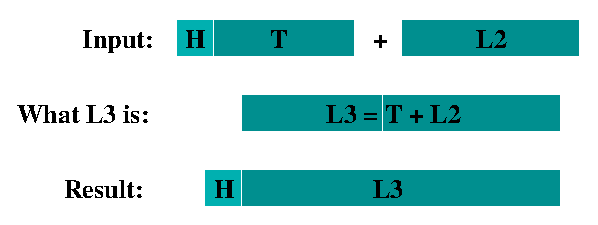
\includegraphics{append.eps}

\begin{quote}
Input:  [ H $\mid$ \fbox{\ T \ } ] + \fbox{\ L2 \ } \\[5mm]
Result: [ H $\mid \underbrace{\fbox{\ L3 \ }}_{\fbox{T}+\fbox{L2}}$ ]
\end{quote}








But what is the procedural meaning of this definition?  What actually
goes on when we use �append/3� to glue two lists together?
Let's take a detailed look at what happens when we pose the query
�?- append([a,b,c],[1,2,3],X)�.

When we pose this query, Prolog will match it to the
head of the recursive rule, generating a new internal variable
(say �_G518�) in the process. If we carried out a trace of what
happens next, we would get something like the following:

\begin{LPNcodedisplay}
append([a, b, c], [1, 2, 3], _G518)
append([b, c], [1, 2, 3], _G587)
append([c], [1, 2, 3], _G590)
append([], [1, 2, 3], _G593)
append([], [1, 2, 3], [1, 2, 3])
append([c], [1, 2, 3], [c, 1, 2, 3])
append([b, c], [1, 2, 3], [b, c, 1, 2, 3])
append([a, b, c], [1, 2, 3], [a, b, c, 1, 2, 3])

X = [a, b, c, 1, 2, 3]
yes
\end{LPNcodedisplay}

The basic pattern should be clear: in the first four lines we see that
Prolog recurses its way down the list in its first argument until it
can apply the base case of the recursive definition.  Then, as the
next four lines show, it then stepwise `fills in' the result.  How is
this `filling in' process carried out?  By successively instantiating
the variables �_G593�, �_G590�, �_G587�, and
�_G518�. But while it's important to grasp this basic pattern, it
doesn't tell us all we need to know about the way �append/3� works,
so let's dig deeper. Here is the search tree for the query
�append([a,b,c],[1,2,3],X)�. We'll work carefully through
all the steps, making a careful note of what our goals are,
and what the variables are instantiated to.

\begin{center}
\includegraphics{chap6-pspic1.ps}
\end{center}


\begin{enumerate}

\item{}Goal 1: �append([a,b,c],[1,2,3],_G518)�.  Prolog
matches this to the head of the recursive rule (that is,
�append([H|T],L2,[H|L3])�).  Thus �_G518� is unified to
�[a|L3]�, and Prolog has the new goal
�append([b,c],[1,2,3],L3)�.
It generates a new variable �_G587� for
�L3�, thus we have that �_G518 = [a|_G587]�.

\item{}Goal 2: �append([b,c],[1,2,3],_G587)�.  Prolog matches
this to the head of the recursive rule, thus �_G587� is unified
to �[b|L3]�, and Prolog has the new goal
�append([c],[1,2,3],L3)�.
It generates the internal variable �_G590� for
�L3�, thus we have that �_G587 = [b|_G590]�.

\item{}Goal 3: �append([c],[1,2,3],_G590�).  Prolog matches this
to the head of the recursive rule, thus �_G590� is unified  to
�[c|L3]�, and Prolog has the new goal
�append([],[1,2,3],L3)�.
It generates the internal variable �_G593� for �L3�,
thus we have that �_G590 = [c|_G593]�.

\item{}Goal 4: �append([],[1,2,3],_G593�).  At last: Prolog
can use the base clause (that is, �append([],L,L)�).  And in the
four successive matching steps, Prolog will obtain answers to Goal 4,
Goal 3, Goal 2, and Goal 1. Here's how.

\item{}Answer to Goal 4: �append([],[1,2,3],[1,2,3])�. This
is because when we match Goal 4 (that is,
�append([],[1,2,3],_G593)� to the base clause, �_G593� is
unified to �[1,2,3]�.

\item{}Answer to Goal 3: �append([c],[1,2,3],[c,1,2,3])�.  Why?
Because Goal 3 is �append([c],[1,2,3],_G590])�, and �_G590� is the
list �[c|_G593]�, and we have just unified �_G593� to �[1,2,3]�. So
�_G590� is unified to �[c,1,2,3]�.

\item{}Answer to Goal 2: �append([b,c],[1,2,3],[b,c,1,2,3])�.
Why? Because Goal 2 is �append([b,c],[1,2,3],_G587])�, and
�_G587� is the list  �[b|_G590]�, and we have just unified �_G590� to
�[c,1,2,3]�. So �_G587� is unified to �[b,c,1,2,3]�.

\item{}Answer to Goal 1: �append([a,b,c],[1,2,3],[a,b,c,1,2,3])�.
Why? Because Goal 2 is �append([a,b,c],[1,2,3],_G518])�,  and
�_G518� is the list �[a|_G587]�, and we have just unified �_G587� to
�[b,c,1,2,3]�. So �_G518� is unified to �[a,b,c,1,2,3]�.

\item{}Thus Prolog now knows how to instantiate �X�, the original
query variable.  It tells us that �X = [a,b,c,1,2,3]�, which
is what we want.
\end{enumerate}


Work through this example carefully, and make sure you fully
understand the pattern of variable instantiations, namely:
\begin{LPNcodedisplay}
_G518 = [a|_G587]
      = [a|[b|_G590]]
      = [a|[b|[c|_G593]]]
\end{LPNcodedisplay}
This type of pattern lies at the heart of the way �append/3� works.
Moreover, it illustrates a more general theme: the use of unification to
build structure. In a nutshell, the recursive calls to �append/3� build up
this nested pattern of variables which code up the required
answer. When Prolog finally instantiates the innermost variable
�_G593� to �[1, 2, 3]�, the answer crystallises out, like a snowflake
forming around a grain of dust. But it is unification, not magic, that
produces the result.



\subsection*{Using append}\label{SUBSEC.L6.USING.APPEND}



Now that we understand how �append/3� works,
let's see how we can put it to work.

One important use of �append/3� is to split up a list into two
consecutive lists.  For example:
\begin{LPNcodedisplay}
?- append(X,Y,[a,b,c,d]).

X = []
Y = [a,b,c,d] ;

X = [a]
Y = [b,c,d] ;

X = [a,b]
Y = [c,d] ;

X = [a,b,c]
Y = [d] ;

X = [a,b,c,d]
Y = [] ;

no
\end{LPNcodedisplay}

That is, we give the list we want to split up (here�[a,b,c,d]�)
to �append/3� as the third argument, and we use variables for the
first two arguments.  Prolog then searches for ways of instantiating
the variables to two lists that concatenate to give the third
argument, thus splitting up the list in two. Moreover, as this example
shows, by backtracking, Prolog can find all possible ways of splitting
up a list into two consecutive lists.

This ability means it is easy to define some useful predicates with
�append/3�.  Let's consider some examples.  First, we can define a
program which finds \LPNterm{prefixes} of lists.  For example, the
prefixes of �[a,b,c,d]� are �[]�, �[a]�, �[a,b]�,
�[a,b,c]�, and �[a,b,c,d]�.  With the help of �append/3�
it is straightforward to define a program �prefix/2�, whose
arguments are both lists, such that �prefix(P,L)� will hold when
�P� is a prefix of �L�.  Here's how:
\begin{LPNcodedisplay}
prefix(P,L):- append(P,_,L).
\end{LPNcodedisplay}

This says that list �P� is a prefix of list �L� when there
is some list such that �L� is the result of concatenating
�P� with that list.  (We use the anonymous variable since we
don't care what that other list is: we only care that there is some such
list or other.) This predicate successfully finds prefixes of lists,
and moreover, via backtracking, finds them all:
\begin{LPNcodedisplay}
?- prefix(X,[a,b,c,d]).

X = [] ;

X = [a] ;

X = [a,b] ;

X = [a,b,c] ;

X = [a,b,c,d] ;

no
\end{LPNcodedisplay}


In a similar fashion, we can define a program which finds
\LPNterm{suffixes} of lists.  For example, the suffixes of
�[a,b,c,d]� are �[]�, �[d]�, �[c,d]�,
�[b,c,d]�, and �[a,b,c,d]�.  Again, using �append/3� it
is easy to define �suffix/2�, a predicate whose arguments
are both lists, such that �suffix(S,L)� will hold when �S�
is a suffix of �L�:
\begin{LPNcodedisplay}
suffix(S,L):- append(_,S,L).
\end{LPNcodedisplay}
That is, list �S� is a suffix of list �L� if there is some
list such that �L� is the result of concatenating that list with
�S�.  This predicate successfully finds suffixes of lists, and
moreover, via backtracking, finds them all:
\begin{LPNcodedisplay}
?- suffix(X,[a,b,c,d]).

X = [a,b,c,d] ;

X = [b,c,d] ;

X = [c,d] ;

X = [d] ;

X = [] ;

no
\end{LPNcodedisplay}

Make sure you understand why the results come out in this order.

\bigskip

And now it's very easy to define a program that finds
\LPNterm{sublists} of lists.  The sublists of �[a,b,c,d]� are �[]�,
�[a]�, �[b]�, �[c]�, �[d]�, �[a,b]�,
�[b,c]�, �[c,d]�, �[a,b,c]�,
�[b,c,d]�, and �[a,b,c,d]�.  A little thought reveals
that the sublists of a list L are simply the \LPNemph{prefixes of suffixes
of} L. Think about it pictorially:


\begin{quote}
Take suffix: \fbox{$a,b,c,d,e,f,g,\underbrace{h,i,j,k,l,m,n,o,p}$}\\[3mm]
Take prefix: \hspace*{23mm}\fbox{$\underbrace{h,i,j,k,l},m,n,o,p$}\\[3mm]
Result:     \hspace*{31mm}\fbox{$h,i,j,k,l$}
\end{quote}


As we already have defined the predicates for producing suffixes and prefixes
of lists, we simply define a sublist as:
\begin{LPNcodedisplay}
sublist(SubL,L):- suffix(S,L), prefix(SubL,S).
\end{LPNcodedisplay}
That is, �SubL� is a sublist of �L� if there is some suffix �S� of �L�
of which �SubL� is a prefix.  This program doesn't
\LPNemph{explicitly} use �append/3�, but of course, under the surface,
that's what's doing the work for us, as both �prefix/2� and �suffix/2� are
defined using �append/3�.




\section{Reversing a List}\label{SEC.L6.REVERSE}

The �append/3� predicate is useful, and it is important to know how to
put it to work. But it is just as important to know that it can be a
source of inefficiency, and that you probably don't want to use it all
the time.

Why is �append/3� a source of inefficiency?  If you think about
the way it works, you'll notice a weakness: �append/3� doesn't join
two lists in one simple action. Rather, it needs to work its way down
its first argument until it finds the end of the list, and only then
can it carry out the concatenation.

Now, often this causes no problems. For example, if we have two lists
and we just want to concatenate them, it's probably not too bad. Sure,
Prolog will need to work down the length of the first list, but if the
list is not too long, that's probably not too high a price
to pay for the ease of working with �append/3�.

But matters may be very different if the first two arguments are given
as variables. As we've just seen, it can be very useful to give
�append/3� variables in its first two arguments, for this lets
Prolog search for ways of splitting up the lists. But there is a price
to pay: a lot of searching is going on, and this can lead to very
inefficient programs.

To illustrate this, we shall examine the problem of reversing a list.
That is, we will examine the problem of defining a predicate which
takes a list (say �[a,b,c,d]�) as input and returns a list
containing the same elements in the reverse order (here
�[d,c,b,a]�).

Now, a reverse predicate is a useful predicate to have around. As you
will have realised by now, lists in Prolog are far easier to access
from the front than from the back. For example, to pull out the head
of a list �L�, all we have to do is perform the unification
�[H|_] = L�; this results in �H� being instantiated to the head of �L�. But
pulling out the last element of an arbitrary list is harder: we can't
do it simply using unification.  On the other hand, if we had a
predicate which reversed lists, we could first reverse the input list,
and then pull out the head of the reversed list, as this would give us
the last element of the original list.  So a reverse predicate could
be a useful tool.  However, as we may have to reverse large lists, we
would like this tool to be efficient.  So we need to think about the
problem carefully.

And that's what we're going to do now.  We will define two reverse
predicates: a naive one, defined with the help of �append/3�, and a
more efficient (and indeed, more natural) one defined using
accumulators.

\subsection*{Naive reverse using append}\label{SUBSEC.L6.REVERSE.NAIVE}



Here's a recursive definition of what is involved in reversing a list:

\begin{enumerate}
\item{}If we reverse the empty list, we obtain the
        empty list.
\item{}If we reverse the list �[H|T]�, we end up with the list
        obtained by reversing �T� and concatenating with �[H]�.
\end{enumerate}
To see that the recursive clause is correct, consider the list
�[a,b,c,d]�.  If we reverse the tail of this list we obtain
�[d,c,b]�.  Concatenating this with �[a]� yields
�[d,c,b,a]�, which is the reverse of �[a,b,c,d]�.

With the help of �append/3� it is easy to turn this recursive
definition into Prolog:

\begin{LPNcodedisplay}
naiverev([],[]).
naiverev([H|T],R):- naiverev(T,RevT), append(RevT,[H],R).
\end{LPNcodedisplay}

Now, this definition is correct, but it does an awful lot of work.
It is \LPNemph{very} instructive to look at a trace of this program.  This
shows that the program is spending a lot of time carrying out appends.
This shouldn't be too surprising: after, all, we are calling
�append/3� recursively.  The result is very
inefficient (if you run a trace, you will find that it takes about 90
steps to reverse an eight element list) and hard to understand (the
predicate spends most of its time in the recursive calls to
�append/3�, making it very hard to see what is going on).

Not nice. But as we shall now see, there \LPNemph{is} a better way.



\subsection*{Reverse using an accumulator}\label{SUBSEC.L6.REVERSE.ACC}

The better way is to use an accumulator.  The underlying idea is
simple and natural.  Our accumulator will be a list, and when we start
it will be empty.  Suppose we want to reverse �[a,b,c,d]�.  At
the start, our accumulator will be �[]�.  So we simply take the
head of the list we are trying to reverse and add it as the head of
the accumulator.  We then carry on processing the tail, thus we are
faced with the task of reversing �[b,c,d]�, and our accumulator
is �[a]�.  Again we take the head of the list we are trying to
reverse and add it as the head of the accumulator (thus our new
accumulator is �[b,a]�) and carry on trying to reverse �[c,d]�.
Again we use the same idea, so we get a new accumulator
�[c,b,a]�, and try to reverse �[d]�.  Needless to say, the
next step yields an accumulator �[d,c,b,a]� and the new goal of
trying to reverse �[]�.  This is where the process stops: \LPNemph{and
our accumulator contains the reversed list we want}.  To summarise:
the idea is simply to work our way through the list we want to
reverse, and push each element in turn onto the head of the
accumulator, like this:
\begin{LPNcodedisplay}
List: [a,b,c,d]  Accumulator: []
List: [b,c,d]    Accumulator: [a]
List: [c,d]      Accumulator: [b,a]
List: [d]        Accumulator: [c,b,a]
List: []         Accumulator: [d,c,b,a]
\end{LPNcodedisplay}
This will be efficient because we simply blast our way through the list once:
we don't have to waste time carrying out concatenation or other
irrelevant work.

It's also easy to put this idea in Prolog.  Here's the accumulator
code:
\begin{LPNcodedisplay}
accRev([H|T],A,R):- accRev(T,[H|A],R).
accRev([],A,A).
\end{LPNcodedisplay}
This is classic accumulator code: it follows the same pattern
as the arithmetic examples we examined in the previous chapter.  The
recursive clause is responsible for chopping off the head of the input
list, and pushing it onto the accumulator.  The base case halts the
program, and copies the accumulator to the final argument.

As is usual with accumulator code, it's a good idea to write a
predicate which carries out the required initialisation of the
accumulator for us:
\begin{LPNcodedisplay}
rev(L,R):- accRev(L,[],R).
\end{LPNcodedisplay}

Again, it is instructive to run some traces on this program and
compare it with �naiverev/2�.  The accumulator based version is
\LPNemph{clearly} better. For example, it takes about 20 steps to reverse
an eight element list, as opposed to 90 for the naive version.
Moreover, the trace is far easier to follow. The idea underlying the
accumulator based version is simpler and more natural than the
recursive calls to �append/3�.


Summing up, �append/3� is a useful program, and you certainly should not
be scared of using it. However, you also need to be aware that it is a
source of inefficiency, so when you use it, ask yourself whether there
is a better way.  And often there is. The use of accumulators is often
better, and (as the �rev/2� example show) accumulators can be a
natural way of handling list processing tasks.

\section{Exercises}\label{SEC.L6.EXERCISES}


\begin{LPNexercise}{L6.EX1}Let's call a list \LPNemph{doubled}
if it is made of two consecutive blocks of elements that are
exactly the same.
For example, �[a,b,c,a,b,c]� is doubled (it's
made up of �[a,b,c]� followed by �[a,b,c]�)
and so is �[foo,gubble,foo,gubble]�. On the other hand,
�[foo,gubble,foo]� is not doubled. Write a predicate
�doubled(List)� which succeeds when �List�
is a doubled list.\end{LPNexercise}
\begin{LPNexercise}{L6.EX2}A palindrome is a word or phrase that spells the same forwards and
backwards.  For example, `rotator', `eve', and `nurses run' are all
palindromes.  Write a predicate �palindrome(List)�, which checks
whether �List� is a palindrome. For example, to the queries
\begin{LPNcodedisplay}
?- palindrome([r,o,t,a,t,o,r]).
\end{LPNcodedisplay}
and
\begin{LPNcodedisplay}
?- palindrome([n,u,r,s,e,s,r,u,n]).
\end{LPNcodedisplay}
Prolog should respond yes, but to the query
\begin{LPNcodedisplay}
?- palindrome([n,o,t,h,i,s]).
\end{LPNcodedisplay}
it should respond no.\end{LPNexercise}



\begin{LPNexercise}{L6.EX3c}
Write a predicate �toptail(InList,OutList)� which says
no if �InList� is a list containing fewer than 2 elements, and
which deletes the first and the last elements of �InList� and
returns the result as �OutList�, when �InList� is a
list containing at least 2 elements. For example:
\begin{LPNcodedisplay}
    toptail([a],T).
    no

    toptail([a,b],T).
    T=[]

    toptail([a,b,c],T).
    T=[b]
\end{LPNcodedisplay}

(Hint: here's where �append/3� comes in useful.)
\end{LPNexercise}

\begin{LPNexercise}{L6.EX3d}
Write a predicate �last(List,X)� which is true only when �List� is a
list that contains at least one element and �X� is the last element of
that list. Do this in two different ways:
\begin{enumerate}
\item Define �last/2� using the predicate �rev/2� discussed in the text.
\item Define �last/2� using recursion.
\end{enumerate}
\end{LPNexercise}

\begin{LPNexercise}{L6.EX3e}
Write a predicate �swapfl(List1,List2)� which checks whether �List1�
is identical to �List2�, except that the first and last elements are
exchanged.  Here's where �append/3� could come in useful again, but it
is also possible to write a recursive definition without appealing to
�append/3� (or any other) predicates.
\end{LPNexercise}





\begin{LPNexercise}{L6.EX4}
Here is an exercise for those of you who like logic
puzzles.

There is a street with three neighbouring houses that all have a
different colour, namely red, blue, and green. People of different
nationalities live in the different houses and they all have a
different pet. Here are some more facts about them:
\begin{itemize}
\item{}The Englishman lives in the red house.
\item{}The jaguar is the pet of the Spanish family.
\item{}The Japanese lives to the right of the snail keeper.
\item{}The snail keeper lives to the left of the blue house.
\end{itemize}
Who keeps the zebra? Don't work it out for yourself:
define a predicate �zebra/1� that tells you the nationality
of the owner of the zebra!

(Hint: Think of a representation for the houses and the street. Code the
four constraints in Prolog. You may find �member/2� and �sublist/2�
useful.)
\end{LPNexercise}


\section{Practical Session}\label{SEC.L6.PRAXIS}



The purpose of Practical Session 6 is to help you get more experience
with list manipulation.  We first suggest some traces for you to carry
out, and then some programming exercises.

The following traces will help you get to grips with the
predicates  discussed in the text:

\begin{enumerate}

\item{}Carry out traces of �append/3� with the
first two arguments instantiated, and the third argument
uninstantiated. For example, �append([a,b,c],[[],[2,3],b],X)�
Make sure the basic pattern is clear.

\item{}Next, carry out traces on �append/3� as used to split up a
list, that is, with the first two arguments given as variables, and the
last argument instantiated. For example,
�append(L,R,[foo,wee,blup]).�

\item{}Carry out some traces on �prefix/2� and �suffix/2�. Why
does �prefix/2� find shorter lists first, and
�suffix/2� longer lists first?

\item{}Carry out some traces on �sublist/2�. As we said in the text,
via backtracking this predicate generates all possible sublists, but
as you'll see, it generates several sublists more than once. Do you
understand why?

\item{}Carry out traces on both �naiverev/2� and �rev/2�, and
compare their behaviour.
\end{enumerate}


Now for some programming work:

\begin{enumerate}
\item{}It is possible to write a one line definition of the
�member� predicate by making use of �append/3�. Do so. How
does this new version of �member� compare in efficiency with the
standard one?
\item{}Write a predicate �set(InList,OutList)� which takes as
input an arbitrary list, and returns a list in which each element of
the input list appears only once. For example, the query
\begin{LPNcodedisplay}

set([2,2,foo,1,foo, [],[]],X).
\end{LPNcodedisplay}

should yield the
result
\begin{LPNcodedisplay}

X = [2,foo,1,[]].
\end{LPNcodedisplay}

(Hint: use  the �member� predicate to test for repetitions
of items you have already found.)

\item{}We `flatten' a list by removing all the square brackets around
any lists it contains as elements, and around any lists that its
elements contain as elements, and so on, for all nested lists. For
example, when we flatten the list
\begin{LPNcodedisplay}
[a,b,[c,d],[[1,2]],foo]
\end{LPNcodedisplay}

we get the list
\begin{LPNcodedisplay}
[a,b,c,d,1,2,foo]
\end{LPNcodedisplay}

and when we flatten the list
\begin{LPNcodedisplay}
[a,b,[[[[[[[c,d]]]]]]],[[1,2]],foo,[]]
\end{LPNcodedisplay}
we also get
\begin{LPNcodedisplay}
[a,b,c,d,1,2,foo].
\end{LPNcodedisplay}
Write a predicate �flatten(List,Flat)� that holds when the first
argument �List� flattens to the second argument �Flat�.
This should be done without making use of �append/3�.
\end{enumerate}

\medskip

Ok, we're now halfway through the book. And flattening a list is the
Pons Asinorum of Prolog programming. Did you cross it ok?  If so,
great. Time to move on.



\chapter{Definite Clause Grammars}\label{CHAPTER7}

\Thischapter{145}{

\noindent
This chapter has two main goals:  
  
\begin{enumerate}
\item{}To introduce context free grammars (CFGs) and some related  
concepts.

\item{}To introduce definite clause grammars (DCGs), a built-in Prolog  
mechanism for working with context free grammars (and other kinds of  
grammar too).
\end{enumerate}

}




\section{Context Free Grammars}\label{SEC.L7.CFG}

Prolog has been used for many purposes, but its inventor, Alain
Colmerauer, was interested in computational linguistics, and this
remains a classic application for the language.  Moreover, Prolog
offers a number of tools which make life easier for computational
linguists, and we are now going to start learning about one of the
most useful of these: \LPNterm{definite clause grammars}, or DCGs as
they are usually called.

 DCGs are a special notation for defining \LPNterm{grammars}.  So,
before we go any further, we'd better learn what a grammar is.  We
shall do so by discussing \LPNterm{context free grammars} (or CFGs).
The basic idea of context free grammars is simple to understand, but
don't be fooled into thinking that CFGs are toys.  They're not.  While
CFGs aren't powerful enough to cope with the syntactic structure of
all natural languages (that is, the kind of languages that human
beings use), they can certainly handle most aspects of the syntax of
many natural languages (for example, English and French) in a
reasonably natural way.

 So what is a context free grammar?  In essence, a finite  
collection of rules which tell us that certain sentences are  
grammatical (that is, syntactically correct) and what their  
grammatical structure actually is.  Here's a simple context free  
grammar for a small fragment of English:  
  
  
\begin{center}\begin{tabular}{l}
�s -> np vp�\\
�np -> det n�\\
�vp -> v np�\\
�vp -> v�\\
�det ->� \LPNemph{a}\\
�det ->� \LPNemph{the}\\
�n ->� \LPNemph{woman}\\
�n ->� \LPNemph{man}\\
�v ->� \LPNemph{shoots}
\end{tabular}\end{center}  
  
What are the ingredients of this little grammar?  Well, first note
that it contains three types of symbol.  There's �->�, which is used
to define the rules.  Then there are the symbols written like this:
�s�, �np�, �vp�, �det�, �n�, �v�. These symbols are called
\LPNterm{non-terminal symbols}; we'll soon learn why.  Each of these
symbols has a traditional meaning in linguistics: �s� is short for
sentence, �np� is short for noun phrase, �vp� is short for verb
phrase, and �det� is short for determiner.  That is, each of these
symbols is shorthand for a grammatical category.  Finally there are
the symbols in italics: \LPNemph{a, the, woman, man}, and
\LPNemph{shoots}.  These are \LPNterm{terminal symbols}, though a
computer scientist might call them the alphabet, and linguists might
call them lexical items.  We'll usually just call them words.

This grammar contains nine \LPNterm{context free rules}.  A context
free rule consists of a single non-terminal symbol, followed by �->�,
followed by a finite sequence made up of terminal and/or non-terminal
symbols.  All nine items listed above have this form, so they are all
legitimate context free rules. What do these rules mean?  They tell us
how different grammatical categories can be built up.  Read �->� as
\LPNemph{can consist of}, or \LPNemph{can be built out of}.  For
example, the first rule tells us that a sentence can consist of a noun
phrase followed by a verb phrase.  The third rule tells us that a verb
phrase can consist of a verb followed by a noun phrase, while the
fourth rule tells us that there is another way to build a verb phrase:
simply use a verb.  The last five rules tell us that \LPNemph{a} and
\LPNemph{the} are determiners, that \LPNemph{man} and \LPNemph{woman}
are nouns, and that \LPNemph{shoots} is a verb.

Now consider the string of words \LPNemph{a woman shoots a man}.  Is   
this grammatical according to our little grammar?  And if it is, what   
structure does it have?  The following tree answers both questions:  

\begin{quote}
  \pstree[levelsep=10mm,nodesep=2mm]{\TR{\texttt{s}}}
    { \pstree[levelsep=10mm,nodesep=2mm]{\TR{\texttt{np}}}
             {\pstree[levelsep=10mm,nodesep=2mm]{\TR{\texttt{det}}}
                     {\TR{\texttt{a}}}
              \pstree[levelsep=10mm,nodesep=2mm]{\TR{\texttt{n}}}
                     {\TR{\texttt{woman}}}}
      \pstree[levelsep=10mm,nodesep=2mm]{\TR{\texttt{vp}}}
             {\pstree[levelsep=10mm,nodesep=2mm]{\TR{\texttt{v}}}
                     {\TR{\texttt{shoots}}}
              \pstree[levelsep=10mm,nodesep=2mm]{\TR{\texttt{np}}}
                     {\pstree[levelsep=10mm,nodesep=2mm]{\TR{\texttt{det}}}
                             {\TR{\texttt{a}}}
                      \pstree[levelsep=10mm,nodesep=2mm]{\TR{\texttt{n}}}
                             {\TR{\texttt{man}}}}}}
\end{quote}

%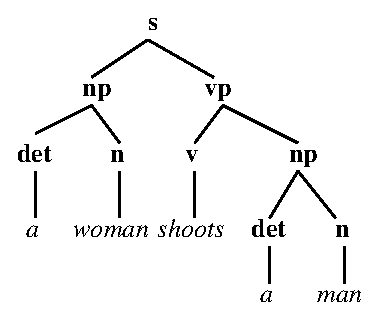
\includegraphics{parse.eps}  

  
Right at the top we have a node marked �s�. This node has two  
daughters, one marked �np�, and one marked �vp�. Note that  
this part of the diagram agrees with the first rule of the grammar,  
which says that an �s� can be built out of an �np� and a  
�vp�. (A linguist would say that this part of the tree is  
\LPNterm{licensed} by the first rule.)  In fact, as you can see,  
\LPNemph{every} part of the tree is licensed by one of our rules.  For  
example, the two nodes marked �np� are licensed by the rule that  
says that an �np� can consist of a �det� followed by an  
�n�. And, right at the bottom of the diagram, all the words in  
\LPNemph{a woman shoots a man} are licensed by a rule. Incidentally, note  
that the terminal symbols only decorate the nodes right at the bottom  
of the tree (the terminal nodes) while non-terminal symbols only  
decorate nodes that are higher up in the tree (the non-terminal  
nodes).

\clearpage
Such a tree is called a \LPNterm{parse tree}. Parse trees are important
because they give us two kinds of information.  Firstly, they give us
information about \LPNterm{strings}. Secondly, they give us information
about \LPNterm{structure}. This is an important distinction to grasp,
so let's have a closer look, and learn some important terminology
while we are doing so.

First, if we are given a string of words, and a grammar, and it turns  
out that we \LPNemph{can} build a parse tree like the one above (that is, a  
tree that has �s� at the top node, and every node in the tree is  
licensed by the grammar, and the string of words we were given is  
listed in the correct order along the terminal nodes) then we say that  
the string is \LPNterm{gramma\-tical} (according to the given grammar).  For  
example, the string \LPNemph{a woman shoots a man} is grammatical according  
to our little grammar (and indeed, any reasonable grammar of English  
would classify it as grammatical). On the other hand, if there isn't  
any such tree, the string is ungrammatical (according to the  
given grammar). For example, the string \LPNemph{woman a woman man a  
shoots} is ungrammatical according to our little grammar (and any  
reasonable grammar of English would classify it as ungrammatical).  
The \LPNterm{language generated by a grammar} consists of all the strings  
that the grammar classifies as grammatical.  For example, \LPNemph{a woman  
shoots a man} also belongs to the language generated by our little  
grammar, and so does \LPNemph{a man shoots the woman}. A context free  
\LPNterm{recogniser} is a program which correctly tells us whether or not a  
string belongs to the language generated by a context free grammar.  
To put it another way, a recogniser is a program that correctly classifies strings  
as grammatical or ungrammatical (relative to some grammar).  

But often, in both linguistics and computer science, we are not merely
interested in whether a string is grammatical or not, we also want to
know \LPNemph{why} it is grammatical.  More precisely, we often want
to know what its structure is, and this is exactly the information a
parse tree gives us. For example, the above parse tree shows us how
the words in \LPNemph{a woman shoots a man} fit together, piece by
piece, to form the sentence.  This kind of information would be
important if we were using this sentence in some application and
needed to say what it actually meant (that is, if we wanted to do
semantics). A context free \LPNterm{parser} is a program which
correctly decides whether a string belongs to the language generated
by a context free grammar \LPNemph{and also tells us what its
structure is}.  That is, whereas a recogniser merely says ``Yes,
grammatical'' or ``No, ungrammatical'' to each string, a parser actually
builds the associated parse tree and gives it to us.

\clearpage
It remains to explain one final concept, namely what a \LPNterm{context
free language} is. (Don't get confused: we've told you what a context
free \LPNemph{grammar} is, but not what a context free
\LPNemph{language} is.)  Quite simply, a context free language is a
language that can be generated by a context free grammar. Some
languages are context free, and some are not. For example, it seems
plausible that English is a context free language. That is, it is
probably possible to write a context free grammar that generates all
(and only) the sentences that native speakers find acceptable. On the
other hand, some dialects of Swiss-German are \LPNemph{not} context
free. It can be proved mathematically that no context free grammar can
generate all (and only) the sentences that native speakers of
Swiss-German find acceptable.%
\footnote{``Evidence against the context-freeness of natural language'', 
Stuart M. Shieber, 
\textit{Linguistics and Philosophy}, 8:333--343, 1985.}
So if you wanted to write a grammar for
such dialects, you would have to employ additional grammatical
mechanisms, not merely context free rules.




\subsection*{CFG recognition using append}\label{SUBSEC.L7.NAIVE.IMPL}



That's the theory, but how do we work with context free grammars in
Prolog?  To make things concrete: suppose we are given a context free
grammar. How can we write a recogniser for it?  And how can we write a
parser for it? In this chapter we'll look at the first question in
detail.  We'll first show how (rather naive) recognisers can be
written in Prolog, and then show how more sophisticated recognisers
can be written with the help of difference lists.  This discussion
will lead us to definite clause grammars, Prolog's built-in grammar
tool.  In the following chapter we'll look at definite clause grammars
in more detail, and learn (among other things) how to use them to
define parsers.

So: given a context free grammar, how do we define a recogniser in  
Prolog?  In fact, Prolog offers a very direct answer to this question:  
we can simply write down Prolog clauses that correspond, in an obvious  
way, to the grammar rules.  That is, we can simply turn the grammar  
into Prolog.

Here's a simple (though as we shall learn, inefficient) way of doing
this.  We shall use lists to represent strings.  For example, we shall
use the list �[a,woman,shoots,a,man]� to represent the string
\LPNemph{a woman shoots a man}.  Now, we have already said that the
�->� symbol used in context free grammars means \LPNemph{can consist
of}, or \LPNemph{can be built out of}, and this idea is easily
modelled using lists.  For example, the rule �s -> np vp� can be
thought of as saying: a list of words is an �s� list if it is the
result of concatenating an �np� list with a �vp� list.  As we know how
to concatenate lists in Prolog (we can use �append/3�), it should be
easy to turn these kinds of rules into Prolog.  And what about the
rules that tell us about individual words?  Even easier: we can simply
view �n ->� \LPNemph{woman} as saying that the list �[woman]� is an
�n� list.

If we turn these ideas into Prolog, this is what we get:  
\begin{LPNcodedisplay}
s(Z):- np(X), vp(Y), append(X,Y,Z).

np(Z):- det(X), n(Y), append(X,Y,Z).

vp(Z):- v(X), np(Y), append(X,Y,Z).

vp(Z):- v(Z).

det([the]).
det([a]).

n([woman]).
n([man]).

v([shoots]).
\end{LPNcodedisplay}
  
  
The correspondence between the CFG rules and the Prolog code should be  
clear.  And to use this program as a recogniser, we simply pose the  
obvious queries.  For example:  
\begin{LPNcodedisplay}
?- s([a,woman,shoots,a,man]).
yes
\end{LPNcodedisplay}
  
In fact, because this is a simple declarative Prolog program, we can  
do more than this: we can also \LPNterm{generate} all the sentences this  
grammar produces.  Our little grammar generates 20 sentences.  
Here are the first five:  
\begin{LPNcodedisplay}
?- s(X).

X = [the,woman,shoots,the,woman] ;

X = [the,woman,shoots,the,man] ;

X = [the,woman,shoots,a,woman] ;

X = [the,woman,shoots,a,man] ;

X = [the,woman,shoots]
\end{LPNcodedisplay}
  
Moreover, we're not restricted to posing questions about sentences: we   
can ask about other grammatical categories. For example:  
\begin{LPNcodedisplay}
?- np([a,woman]).
yes
\end{LPNcodedisplay}
  
And we can generate noun phrases with the following query.  
\begin{LPNcodedisplay}
?- np(X).
\end{LPNcodedisplay}
  
  
Now this is rather nice.  We have a simple, easy to understand program  
which corresponds with our CFG in an obvious way.  Moreover, if we  
added more rules to our CFG, it would be easy to alter the program to  
cope with the new rules.

But there is a problem: the program doesn't use the input sentence to  
guide the search. Make a trace for the query �s([a,man,shoots])�  
and you will see that the program chooses
noun phrases and verb  
phrases and only afterwards checks whether these can be combined to  
form the sentence �[a,man,shoots]�. For example, Prolog will find that  
�[the,woman]� is a noun phrase and �[shoots,the,woman]� a  
verb phrase and only then will it check whether concatenating these  
lists happens to yield �[a,man,shoots]�, which of course  
it won't. So, Prolog starts to backtrack, and the next thing it will try  
is whether concatenating the noun phrase �[the,woman]� and the  
verb phrase �[shoots,the,man]� happens to yield  
�[a,man,shoots]�, another non-starter.
It will go on like this until it (finally)  
produces the noun phrase �[a,man]� and the verb phrase  
�[shoots]�. The problem is that the goals  
�np(X)� and �vp(Y)� are called with uninstantiated variables  
as arguments. 

So, how about changing the rules in such a way that �append�  
becomes the first goal:  
\begin{LPNcodedisplay}
s(Z):- append(X,Y,Z), np(X), vp(Y).

np(Z):- append(X,Y,Z), det(X), n(Y).

vp(Z):-  append(X,Y,Z), v(X), np(Y).

vp(Z):-  v(Z).

det([the]).
det([a]).

n([woman]).
n([man]).

v([shoots]).
\end{LPNcodedisplay}

Here we first use �append/3� to split up the input list. This
instantiates the variables �X� and �Y�, so that the other goals are
all called with instantiated arguments. However, this program is still
not very appealing: it uses �append/3� a lot and, even worse, it uses
�append/3� with uninstantiated variables in the first two
arguments. We saw in the previous chapter that this is a source of
inefficiency. And indeed, the performance of this recogniser is very
bad.  It is revealing to trace through what actually happens when this
program analyses a sentence such as \LPNemph{a woman shoots a man}.
As you will see, relatively few of the steps are devoted to the real
task of recognising the sentences: most are devoted to using
�append/3� to decompose lists.  This isn't much of a problem for our
little grammar, but it certainly would be if we were working with a
more realistic grammar capable of generating a large number of
sentences. We need to do something about this.

\subsection*{CFG recognition using difference lists}\label{SUBSEC.L7.DIFF.STRUCTURES}



A more efficient implementation can be obtained by making use of  
\LPNemph{difference lists}. This is a sophisticated (and, once you've  
grasped it, beautiful) Prolog technique that can be used for a  
variety of purposes.  


The key idea underlying difference lists is to represent the
information about grammatical categories not as a single list, but as
the difference between two lists.  For example, instead of
representing \LPNemph{a woman shoots a man} as
�[a,woman,shoots,a,man]� we can represent it as the pair of lists
\begin{LPNcodedisplay}
[a,woman,shoots,a,man] [].  
\end{LPNcodedisplay}
 Think of the first list as  
\LPNemph{what needs to be consumed} (or if you prefer:  the \LPNemph{input  
list}), and the second list as \LPNemph{what we should leave behind} (or:  
the \LPNemph{output list}).  Viewed from this (rather procedural) perspective  
the difference list  
\begin{LPNcodedisplay}
[a,woman,shoots,a,man] []. 
\end{LPNcodedisplay}
 represents the sentence \LPNemph{a woman  
shoots a man} because it says:  
\LPNemph{If I consume all the symbols on the left, and leave  
        behind the symbols on the right, then I have the sentence  
        I am interested in.}
That is, the sentence we are interested in is the difference   
between the contents of these two lists.



That's all we need to know about difference lists to rewrite our
recogniser. If we simply bear in mind the idea of consuming something,
and leaving something behind in mind, we obtain the following
recogniser:
\begin{LPNcodedisplay}
s(X,Z):- np(X,Y), vp(Y,Z).

np(X,Z):- det(X,Y), n(Y,Z).

vp(X,Z):-  v(X,Y), np(Y,Z).

vp(X,Z):-  v(X,Z).

det([the|W],W).
det([a|W],W).

n([woman|W],W).
n([man|W],W).

v([shoots|W],W).
\end{LPNcodedisplay}
  
Consider these rules carefully. For example, the �s� rule says:
\LPNemph{I know that the pair of lists} �X� \LPNemph{and} �Z�
\LPNemph{represents a sentence if (1) I can consume} �X� \LPNemph{and
leave behind a} �Y�, \LPNemph{and the pair} �X� \LPNemph{and} �Y�
\LPNemph{represents a noun phrase, and (2) I can then go on to
consume} �Y� \LPNemph{leaving Z behind}, \LPNemph{and the pair} �Y�
�Z� \LPNemph{represents a verb phrase}. The  �np� rule and the
second of the �vp� rules work similarly.

Moreover, the same idea underlies the way this grammar handles the
words. For example
\begin{LPNcodedisplay}
n([man|W],W).
\end{LPNcodedisplay}
means we are handling \LPNemph{man} as the difference between
�[man|W]� and �W�.  After all, the difference between what is consumed
and what is left behind is precisely the word �man�.

Now, at first this code may be harder to grasp than our previous
recogniser. But note that we have gained something important:
\LPNemph{we haven't used} �append/3�. In the difference list based
recogniser, it simply isn't needed, and this makes a big difference.

How do we use this recogniser? Well, here's how to recognise
sentences:
\begin{LPNcodedisplay}
?- s([a,woman,shoots,a,man],[]).
yes
\end{LPNcodedisplay}
This asks whether we can get an �s� by consuming the symbols   
in �[a,woman,shoots,a,man]�, leaving nothing behind.
Similarly, to generate all the sentences in the grammar,  
we ask  
\begin{LPNcodedisplay}
?- s(X,[]).
\end{LPNcodedisplay}
This asks: what values can you give to �X�, such that we get an �s� by
consuming the symbols in �X�, leaving nothing behind?

The queries for other grammatical categories also work the same way.    
For example, to find out if \LPNemph{a woman} is a noun phrase we ask:  
\begin{LPNcodedisplay}
?- np([a,woman],[]).
\end{LPNcodedisplay}
And we generate all the noun phrases in the grammar as follows:  
\begin{LPNcodedisplay}
?- np(X,[]).
\end{LPNcodedisplay}


You should trace what happens when this program analyses a sentence
such as \LPNemph{a woman shoots a man}.  As you will see, it is a lot
more efficient than our �append/3� based program.  Moreover, as no use
is made of �append/3�, the trace is a lot easier to grasp.  So we have
taken a big step forward.

On the other hand, it has to be admitted that the second recogniser is  
not as easy to understand, at least at first, and it's a pain having  
to keep track of all those difference list variables.  If only it were  
possible to have a recogniser as simple as the first and as efficient  
as the second. And in fact, it \LPNemph{is} possible: this is  where  
DCGs come in.



\section{Definite Clause Grammars}\label{SEC.L7.DCG}

So, what are DCGs?  Quite simply, a nice notation for writing  
grammars that hides the underlying difference list variables.  
Let's look at three examples.  
  


\subsection*{A first example}\label{SUBSEC.L7.FIRSTEXAMPLE}

As our first example, here's our little  
grammar written as a DCG:  
  
\begin{LPNcodedisplay}
s --> np,vp.

np --> det,n.

vp --> v,np.
vp --> v.

det --> [the].
det --> [a].

n --> [woman].
n --> [man].

v --> [shoots].
\end{LPNcodedisplay}

The link with the original context free grammar should be transparent:
this is definitely the most user-friendly notation we have used yet.
But how do we use this DCG? In fact, we use it in \LPNemph{exactly}
the same way as we used our difference list recogniser.  For example,
to find out whether \LPNemph{a woman shoots a man} is a sentence, we
pose the query:
  
\begin{LPNcodedisplay}
?- s([a,woman,shoots,a,man],[]).
\end{LPNcodedisplay}
That is, just as in the difference list recogniser, we ask   
whether we can get an �s� by consuming the symbols in   
�[a,woman,shoots,a,man]�, leaving nothing behind.

Similarly, to generate all the sentences in the grammar,  
we pose the query:  
\begin{LPNcodedisplay}
?- s(X,[]).
\end{LPNcodedisplay}
This asks what values we can give to �X�, such that we get an  
�s� by consuming the symbols in �X�, leaving nothing behind.

Moreover, the queries for other grammatical categories also work the   
same way.  For example, to find out if \LPNemph{a woman} is a noun phrase   
we pose the query:  
\begin{LPNcodedisplay}
?- np([a,woman],[]).
\end{LPNcodedisplay}
And we generate all the noun phrases in the grammar as follows:  
\begin{LPNcodedisplay}
?- np(X,[]).
\end{LPNcodedisplay}
  
  
What's going on?  Quite simply, this DCG \LPNemph{is} our difference
list recogniser!  To put it another way, DCG notation is essentially
syntactic sugar, user-friendly notation that lets us write grammars in
a natural way.  But Prolog translates this notation into the kinds of
difference lists discussed before.  So we have the best of both
worlds: a nice simple notation for working with, and the
efficiency of difference lists.

There is an easy way to see what Prolog translates DCG rules into.
Suppose you are working with the DCG just given (that is, suppose that
Prolog has already consulted the rules).  Then if you pose the query:
\begin{LPNcodedisplay}
?- listing(s).
\end{LPNcodedisplay}
you will get the response  
\begin{LPNcodedisplay}
s(A,B) :-
    np(A,C),
    vp(C,B).
\end{LPNcodedisplay}
This is what Prolog has translated �s --> np,vp� into. Note  
that (apart from the choice of variables) this is exactly the  
difference list rule we used in our second recogniser.

Similarly, if you pose the query  
\begin{LPNcodedisplay}
?- listing(np).
\end{LPNcodedisplay}
you will get  
\begin{LPNcodedisplay}
np(A,B) :-
    det(A,C),
    n(C,B).
\end{LPNcodedisplay}
This is what Prolog has translated �np --> det,n� into. Again  
(apart from the choice of variables) this is  the  
difference list rule we used in our second recogniser.

To get a complete listing of the translations of all the rules, simply  
type  
\begin{LPNcodedisplay}
?- listing.
\end{LPNcodedisplay}
There is one thing you may observe. Some Prolog implementations  
translate rules such as  
\begin{LPNcodedisplay}
det --> [the].
\end{LPNcodedisplay}
not into  
\begin{LPNcodedisplay}
det([the|W],W).
\end{LPNcodedisplay}
which was the form we used in our difference list recogniser, but into  
\begin{LPNcodedisplay}
det(A,B) :-
    'C'(A,the,B).
\end{LPNcodedisplay}
But although the notation is different, the idea is the same.  This
says you can get a list �B� from a list �A� by consuming a �the�.
That is, once again this is a difference list representation.  Note
that �'C'� is an atom. \index{PROLOG c/3@\texttt{'C'/3}}


\subsection*{Adding recursive rules}\label{SUBSEC.L7.RECURSIVE.RULES}


Our original context free grammar generated only 20 sentences.  
However it is easy to write context free grammars that generate  
infinitely many sentences: simply use recursive rules. Here's  
an example. Let's add the following rules to our little grammar:  
  
\begin{center}\begin{tabular}{l}
�s -> s conj s�\\
�conj ->� \LPNemph{and}\\
�conj ->� \LPNemph{or}\\
�conj ->� \LPNemph{but}
\end{tabular}\end{center}  
This rule allows us to join as many sentences together as we like
using the words \LPNemph{and}, \LPNemph{but}, and \LPNemph{or}. So this
grammar classifies sentences such as \LPNemph{The woman shoots the man
or the man shoots the woman} as grammatical.

Now, in principle it is easy to turn this grammar into a DCG. We
need merely add the rules
\begin{LPNcodedisplay}
s --> s,conj,s.

conj --> [and].
conj --> [or].
conj --> [but].
\end{LPNcodedisplay}
But there is a problem lurking under the surface. What does Prolog
actually \LPNemph{do} with this DCG? Let's have a look.

First, let's add the new rules at the \LPNemph{beginning} of the
knowledge base, before the rule �s --> np,vp�. What happens if we then
pose the query �s([a,woman,shoots],[])�? Prolog immediately goes into
a loop.

Can you see why? The point is this. Prolog translates DCG rules into  
ordinary Prolog rules. If we place the recursive rule   
�s --> s,conj,s� in the knowledge base before the non-recursive  
rule   
�s --> np,vp� then the knowledge base will contain the following two  
Prolog rules, in this order:  
\begin{LPNcodedisplay}
s(A, B) :-
        s(A, C),
        conj(C, D),
        s(D, B).

s(A, B) :-
        np(A, C),
        vp(C, B).
\end{LPNcodedisplay}
Now, from a declarative perspective this is fine, but from a
procedural perspective this is fatal.  When it tries to use the first
rule, Prolog immediately encounters the goal �s(A,C)�, which it then
tries to satisfy using the first rule, whereupon it immediately
encounters the goal �s(A, C)�, which it then tries to satisfy using
the first rule, whereupon it immediately encounters the goal �s(A, C)�,
and so on. In short, it goes into an infinite loop and does no
useful work.

So let's add the recursive rule �s --> s,conj,s� at the end of the
knowledge base, so that Prolog always encounters the translation of
the non-recursive rule first. What happens now, when we pose the query
�s([a,woman,shoots],[])�? Well, now Prolog handles this and gives an
answer. But what happens when we pose the query �s([woman,shoot],[])�?
Note that this is an ungrammatical sentence that is not accepted by
our grammar. Once again, Prolog gets into an infinite loop. Since it
is impossible to recognise �[woman,shoot]� as a sentence consisting of
a noun phrase and a verb phrase, Prolog tries to analyse it with the
rule �s --> s,conj,s�, and ends up in the same unending loop as
before.

In short, we are having the same problems that we met when we
discussed recursion, and rule and goal ordering, in
Chapter~\ref{CHAPTER3}.  In a nutshell, �s --> s,conj,s� translates
into a left-recursive rule, and that's bad news.  Moreover, as we saw
earlier, we \textit{can't} fix such problems simply by tinkering with
the rule ordering: the way out of such difficulties is to change the
goal order of the recursive rule so that the recursive goal is not the
first one in the body of the rule. That is, ideally we should rewrite
the rule so that it is no longer left-recursive.

Nice idea, but unfortunately, it is not an option here.  Why not?
Because the order of the goals determines the order of the words in
the sentence!  It makes an important difference, for example, whether
our grammar accepts \LPNemph{the woman shoots the man and the man
shoots the woman} (�s --> s,conj,s�) or whether it accepts
\LPNemph{and the woman shoots the man the man shoots the woman} (�s --> conj,s,s�).

But there is a way out.
The standard solution is to introduce a new non-terminal symbol and
rewrite the DCG.  We could, for example, use the category �simple_s�
for sentences without embedded sentences. Our grammar would then look
like this:
\begin{LPNcodedisplay}
s --> simple_s.
s --> simple_s,conj,s.
simple_s --> np,vp.
np --> det,n.
vp --> v,np.
vp --> v.
det --> [the].
det --> [a].
n --> [woman].
n --> [man].
v --> [shoots].
conj --> [and].
conj --> [or].
conj --> [but].
\end{LPNcodedisplay}
As you should check, Prolog doesn't get into infinite loops with this
grammar as it did with the previous one, so from a computational
perspective the solution is satisfactory. But it leaves something to
be desired from a linguistic perspective. The DCG that looped was at
least faithful to the linguistic intuitions about the structure of
sentences made using \textit{and}, \textit{but}, and \textit{or}.  The
new DCG imposes an additional layer of structure that is motivated by
processing rather than linguistic considerations; we are no longer
simply turning grammars into Prolog.

The moral is: DCGs aren't magic. They are a nice notation, but you
can't expect to write down an arbitrary CFG as a DCG and have it run
without problems. DCG rules are ordinary Prolog rules in disguise, and
this means that you must pay attention to what your Prolog interpreter
is going to do with them. And in particular, you have to keep an eye
out for left-recursion.


\subsection*{A DCG for a simple formal language}\label{SUBSEC.L7.ANBN}

As our last example, we shall define a DCG for the \LPNterm{formal
language} $a^nb^n$. What is this language? And what is a formal
language anyway?

 A formal language is simply a set of strings. The term ``formal
language'' is intended to contrast with the term ``natural language'':
whereas natural languages are languages that human beings actually
use, formal languages are mathematical objects that computer
scientists, logicians, and mathematicians define and study for various
purposes.

A simple example of a formal language is $a^nb^n$.  The words in this
language are built up from two symbols: the symbol \LPNemph{a} and the
symbol \LPNemph{b}.  In fact, the language $a^nb^n$ consists of all
strings made up from these two symbols that have the following form:
the string must consist of an unbroken block of \LPNemph{a}s of length
\LPNemph{n}, followed by an unbroken block of \LPNemph{b}s of length
\LPNemph{n}, and nothing else.  So the strings \LPNemph{ab},
\LPNemph{aabb}, \LPNemph{aaabbb} and \LPNemph{aaaabbbb} all belong to
$a^nb^n$. (Note that the \LPNterm{empty string} belongs to $a^nb^n$
too: after all, the empty string consists of a block of \LPNemph{a}s
of length zero followed by a block of \LPNemph{b}s of length zero.)
On the other hand, \LPNemph{aba} and \LPNemph{abba} do not belong to
$a^nb^n$.

Now, it is easy to write a context free grammar that generates this  
language:  
  
\begin{center}\begin{tabular}{l}
�s -> �$\epsilon$\\
�s -> l s r�\\
�l -> a �\\
�r -> b�
\end{tabular}\end{center}  
  
The first rule says that an \LPNemph{s} can be realised as nothing at
all.  The second rule says that an \LPNemph{s} can be made up of an
\LPNemph{l} (for left) element, followed by an \LPNemph{s}, followed
by an \LPNemph{r} (for right) element. The last two rules say that
\LPNemph{l} elements and \LPNemph{r} elements can be realised as
\LPNemph{a}s and \LPNemph{b}s respectively. It should be clear that
this grammar really does generate all and only the elements of
$a^nb^n$, including the empty string.

Moreover, it is easy to turn this grammar into DCG. We can do so as  
follows:  
\begin{LPNcodedisplay}
s --> [].
s --> l,s,r.

l --> [a].
r --> [b].
\end{LPNcodedisplay}
Note that the second rule is recursive (but, thankfully, not left
recursive).  And in fact this DCG works exactly as we would hope. For
example, to the query
\begin{LPNcodedisplay}
?- s([a,a,a,b,b,b],[]).
\end{LPNcodedisplay}
we get the answer yes, while to the query  
\begin{LPNcodedisplay}
?- s([a,a,a,b,b,b,b],[]).
\end{LPNcodedisplay}
we get the answer no. The query  
\begin{LPNcodedisplay}
?- s(X,[]).
\end{LPNcodedisplay}
enumerates  the strings in the language, starting  
from �[]�.  


\section{Exercises}\label{SEC.L7.EXERCISES}

\begin{LPNexercise}{L7.EX1}Suppose we are working with the following DCG:  
\begin{LPNcodedisplay}
s --> foo,bar,wiggle.
foo --> [choo].
foo --> foo,foo.
bar --> mar,zar.
mar --> me,my.
me --> [i].
my --> [am].
zar --> blar,car.
blar --> [a].
car --> [train].
wiggle --> [toot].
wiggle --> wiggle,wiggle.
\end{LPNcodedisplay}
Write down the ordinary Prolog rules that correspond to these  
DCG rules.  
What are the first three responses that Prolog gives to the query  
�s(X,[])�?
\end{LPNexercise}


\begin{LPNexercise}{L7.EX2}The formal language $a^nb^n - \{\epsilon\}$ consists of all the strings in  
$a^nb^n$ except the empty string. Write a DCG that generates this  
language.
\end{LPNexercise}


\begin{LPNexercise}{L7.EX3}Let $a^nb^{2n}$ be the formal language which contains all strings of  
the following form: an unbroken block of \LPNemph{a}s of length \LPNemph{n}  
followed by an unbroken block of \LPNemph{b}s of length \LPNemph{2n}, and  
nothing else. For example, \LPNemph{abb}, \LPNemph{aabbbb}, and \LPNemph{aaabbbbbb}  
belong to $a^nb^{2n}$, and so does the empty string.  Write a DCG that  
generates this language.  
 \end{LPNexercise}


\section{Practical Session}\label{SEC.L7.PRAXIS}



The purpose of this session is to help you get familiar with DCGs,
difference lists, and the relation between them, and to give you some
experience in writing basic DCGs.  As you will learn in the following
chapter, there is more to DCGs than the ideas just
discussed. Nonetheless, what you have learned so far is certainly the
core, and it is important that you are comfortable with the basic
ideas before moving on.

First some keyboard exercises:  
\begin{enumerate}

\item{}Type in or download the simple �append/3� based recognisers
discussed in the text, and then run some traces.  As you will see, we
were not exaggerating when we said that their performance is
poor. Even for such simple sentences as \LPNemph{The woman shot a man}
you will see that the traces are long and difficult to follow.

\item{}Next, type in or download our second recogniser, the one based  
on difference lists, and run more traces. As you will see, there is a  
dramatic gain in efficiency. Moreover, you will see that the traces  
are \LPNemph{very} simple to understand, especially when compared with the  
monsters produced by the �append/3� based implementations.

\item{}Next, type in or download the DCG discussed in the text.  Type  
�listing� so that you can see what Prolog translates the rules  
to. How does your system translate rules of the form   \index{PROLOG c/3@\texttt{'C'/3}}
�Det --> [the]�? That is, does it translate them to rules like  
�det([the|X],X)�, or does is make use of rules  
containing the \texttt{'C'} predicate?

\item{}Now run some traces. Apart from variable names, the traces you  
observe here should be very similar to the traces you observed when  
running the difference list recogniser. 

\end{enumerate}
  
  
And now it's time to write some DCGs:  
  
\begin{enumerate}
\item{}The formal language \LPNemph{Even} is very simple: it consists of  
all strings containing an even number of \LPNemph{a}s, and nothing else.  
Note that the empty string $\epsilon$ belongs to \LPNemph{Even}.  
Write a DCG that generates \LPNemph{Even}.
\item{}The formal language $a^nb^{2m}c^{2m}d^{n}$ consists of all  
strings of the following form: an unbroken block of \LPNemph{a}s followed  
by an unbroken block of \LPNemph{b}s followed by an unbroken block of  
\LPNemph{c}s followed by an unbroken block of \LPNemph{d}s, such that the \LPNemph{a}  
and \LPNemph{d} blocks are exactly the same length, and the \LPNemph{b} and  
\LPNemph{c} blocks are also exactly the same length and furthermore consist of   
an even number of \LPNemph{b}s and \LPNemph{c}s respectively. For example, $\epsilon$,   
\LPNemph{abbccd}, and \LPNemph{aabbbbccccdd} all belong to  
$a^nb^{2m}c^{2m}d^{n}$.  Write a DCG that generates this  
language.
\item{}The language that logicians call ``propositional logic   
over the propositional symbols \LPNemph{p},  
\LPNemph{q}, and \LPNemph{r}'' can be defined  
by the following context free grammar:  
\begin{center}\begin{tabular}{l}
�prop -> p�\\
�prop -> q�\\
�prop -> r�\\
�prop ->� $\neg$� prop�\\
�prop ->� �(prop �$\wedge$� prop)�\\
�prop ->� �(prop �$\vee$� prop)�\\
�prop ->� �(prop �$\rightarrow$� prop)�
\end{tabular}\end{center}  

Write a DCG that generates this language. Actually, because we don't  
know about Prolog operators yet, you will have to make a few rather  
clumsy looking compromises. For example, instead of getting it to  
recognise  
\begin{center}\begin{tabular}{l}$\neg$�(p � $\rightarrow$� q)�
\end{tabular}\end{center}  
you will have to get it recognise things like  
\begin{center}\begin{tabular}{l}�[not, '(', p, implies, q, ')']�
\end{tabular}\end{center}  
instead. We will learn in Chapter~\ref{CHAPTER9} how to deal with
propositional logic somewhat more naturally; in the meantime, write a
DCG that accepts a clumsy looking version of this language. Use
\LPNemph{or} for $\vee$, and \LPNemph{and} for $\wedge$.
\end{enumerate}




\chapter{More Definite Clause Grammars}\label{CHAPTER8}

\Thischapter{130}{
 
\noindent
This chapter has two main goals:  
  
\begin{enumerate}

\item{}To examine two important capabilities offered by DCG notation:
extra arguments and extra goals.

\item{}To discuss the status and limitations of DCGs.
\end{enumerate}

}




\section{Extra Arguments}\label{SEC.L8.EXTRA.ARGUMENTS}

In the previous chapter we introduced basic DCG notation. But DCGs
offer  more than we've seen so far.  For a start, DCGs allow us to
specify extra arguments.  Extra arguments can be used for many
purposes; we'll examine three.




\subsection*{Context free grammars with features}\label{SUBSEC.L8.GRAMMARS.FEATURES}

 
As a first example, let's see how extra arguments can be used to add  
\LPNemph{features} to context-free grammars.

Here's the  DCG we worked with in the previous chapter:  
  
\begin{LPNcodedisplay}
s --> np,vp.

np --> det,n.

vp --> v,np.
vp --> v.

det --> [the].
det --> [a].

n --> [woman].
n --> [man].

v --> [shoots].
\end{LPNcodedisplay}
  
Now, suppose we wanted to deal with sentences like ``She shoots him'',
and ``He shoots her''.  What should we do?  Well, obviously we should
add rules saying that ``he'', ``she'', ``him'', and ``her'' are
pronouns:
\begin{LPNcodedisplay}
pro --> [he].
pro --> [she].
pro --> [him].
pro --> [her].
\end{LPNcodedisplay}
Furthermore, we should add a rule saying that noun phrases can be   
pronouns:  
\begin{LPNcodedisplay}
np --> pro.
\end{LPNcodedisplay}
  
In this new DCG any good? Well, up to a point, it works. For example:
\begin{LPNcodedisplay}
?- s([she,shoots,him],[]).
yes
\end{LPNcodedisplay}
  
But there's an obvious problem.  The DCG will also accept a lot of   
sentences that are clearly wrong, such as ``A woman shoots she'',   
``Her shoots a man'', and ``Her shoots she'':  
\begin{LPNcodedisplay}
?- s([a,woman,shoots,she],[]).
yes

?- s([her,shoots,a,man],[]).
yes

?- s([her,shoots,she],[]).
yes
\end{LPNcodedisplay}
  
That is, the grammar doesn't know that ``she'' and ``he'' are \LPNemph{subject} pronouns and cannot be used in \LPNemph{object} position;   
thus ``A woman shoots she'' is bad because it violates this basic fact   
about English.  Moreover, the grammar doesn't know that ``her'' and   
``him'' are \LPNemph{object} pronouns and cannot be used in \LPNemph{subject} position; thus ``Her shoots a man'' is bad because it   
violates this constraint.  As for ``Her shoots she'', this manages to   
get both matters wrong at once.

Now, it's pretty obvious \LPNemph{what} we have to do to put this right:   
we need to extend the DCG with information about which pronouns can   
occur in subject position and which in object position.  The   
interesting question: \LPNemph{how} exactly are we to do this?  First   
let's look at a naive way of correcting this, namely adding new rules:  
  
\begin{LPNcodedisplay}
s --> np_subject,vp.

np_subject --> det,n.
np_object  --> det,n.
np_subject --> pro_subject.
np_object  --> pro_object.

vp --> v,np_object.
vp --> v.

det --> [the].
det --> [a].

n --> [woman].
n --> [man].

pro_subject --> [he].
pro_subject --> [she].
pro_object --> [him].
pro_object --> [her].

v --> [shoots].
\end{LPNcodedisplay}
  
  
Now this solution ``works''. For example,   
\begin{LPNcodedisplay}
?- s([her,shoots,she],[]).
no
\end{LPNcodedisplay}
  
But neither computer scientists nor linguists would consider this a
good solution.  The trouble is, a small addition to the lexicon has
led to quite a big change in the DCG. Let's face it: ``she'' and
``her'' (and ``he'' and ``him'') are the same in a lot of respects.
But to deal with the property in which they differ (namely, in which
position they can occur in sentences) we've had to make big changes to
the grammar: in particular, we've doubled the number of noun phrase
rules.  If we had to make further changes (for example, to cope with
plural noun phrases) things would get even worse.  What we really need
is a more delicate programming mechanism that allows us to cope with
such facts without being forced to add rules all the time.  And here's
where the extra arguments come into play.  Look at the following
grammar:
  
\begin{LPNcodedisplay}
s --> np(subject),vp.

np(_) --> det,n.
np(X) --> pro(X).

vp --> v,np(object).
vp --> v.

det --> [the].
det --> [a].

n --> [woman].
n --> [man].

pro(subject) --> [he].
pro(subject) --> [she].
pro(object) --> [him].
pro(object) --> [her].

v --> [shoots].
\end{LPNcodedisplay}
  
  
  
  
The key thing to note is that this new grammar contains only one new
noun phrase rule.  In fact, it is very similar to the first grammar
that we wrote, except that now the symbol �np� is associated with a
new argument, either �subject�, �object�, �_� or �X�.  A
linguist would say that we've added \LPNterm{features} to distinguish
various kinds of noun phrase.  In particular, note the four rules for
the pronouns. Here we've used the extra argument to state which
pronouns can occur in subject position, and which can occur in object
position. Thus these rules are the most fundamental, for they give us
the basic facts about how these pronouns can be used.

So what do the other rules do? Well, intuitively, the rule  
\begin{LPNcodedisplay}
np(X) --> pro(X).
\end{LPNcodedisplay}
uses the extra argument (the variable �X�) to pass these basic facts
about pronouns up to noun phrases built out of them: because the
variable �X� is used as the extra argument for both the np and the
pronoun, Prolog unification will guarantee that they will be given the
same value. In particular, if the pronoun we use is ``she'' (in which
case �X=subject�), then the np will (through its extra argument
�X=subject�) be marked as a subject np. On the other hand, if the
pronoun we use is ``her'' (in which case �X=object�), then the extra
argument for np will be marked �X=object� too. And this, of course, is
exactly the behaviour we want.

On the other hand, although noun phrases built using the rule  
\begin{LPNcodedisplay}
np(_) --> det,n.
\end{LPNcodedisplay}
also have an extra argument, we've used the anonymous variable as its   
value.  Essentially this means \LPNemph{can be either}, which is   
correct, for expressions built using this rule (such as ``the man''   
and ``a woman'') can be used in both subject and object position.  

Now consider the rule  
\begin{LPNcodedisplay}
vp --> v,np(object).
\end{LPNcodedisplay}
This says that to apply this rule we need to use a noun phrase whose  
extra argument unifies with �object�.  This can be \LPNemph{either}  
noun phrases built from object pronouns \LPNemph{or} noun phrases such as  
``the man'' and ``a woman'' which have the anonymous variable as the  
value of the extra argument.  Crucially, pronouns marked has having  
�subject� as the value of the extra argument \LPNemph{can't} be used  
here: the atoms �object� and �subject� don't unify.  Note  
that the rule  
\begin{LPNcodedisplay}
s --> np(subject),vp.
\end{LPNcodedisplay}
works in an analogous fashion to prevent noun phrases made of object   
pronouns from ending up in subject position.

This works.  You can check it out by posing the query:  
\begin{LPNcodedisplay}
?- s(X,[]).     
\end{LPNcodedisplay}
As you step through the responses, you'll see that only acceptable   
English is generated.

But while the intuitive explanation just given is correct, what's
\LPNemph{really} going on?  The key thing to remember is that DCG
rules are just a convenient abbreviation.  For example, the
rule
\begin{LPNcodedisplay}
s --> np,vp.
\end{LPNcodedisplay}
is really syntactic sugar for  
\begin{LPNcodedisplay}
s(A,B) :-
    np(A,C),
    vp(C,B).
\end{LPNcodedisplay}
That is, as we learned in the previous chapter, the DCG notation is a   
way of hiding the two arguments responsible for the difference list   
representation, so that we don't have to think about them.  We work   
with the nice user-friendly notation, and Prolog translates it into   
the clauses just given.

Ok, so we obviously need to ask what  
\begin{LPNcodedisplay}
s --> np(subject),vp.
\end{LPNcodedisplay}
translates into. Here's the answer:  
\begin{LPNcodedisplay}
s(A,B) :-
    np(subject,A,C),
    vp(C,B).
\end{LPNcodedisplay}
  
As should now be clear, the name ``extra argument'' is a good one: as
this translation makes clear, the �subject� symbol really
\LPNemph{is} just one more argument in an ordinary Prolog rule.
Similarly, our noun phrase DCG rules translate into
\begin{LPNcodedisplay}
np(A,B,C) :-
    det(B,D),
    n(D,C).
np(A,B,C) :-
    pro(A,B,C).
\end{LPNcodedisplay}
Note that both rules have \LPNemph{three} arguments.  The first, �A�,
is the extra argument, and the last two are the ordinary, hidden DCG
arguments (the two hidden arguments are always the last two
arguments).

Incidentally, how do you think we would use the grammar to list the   
grammatical noun phrases?  Well, if we had been working with the DCG   
rule �np --> det,n� (that is, a rule with no extra arguments)   
we would have made the query  
\begin{LPNcodedisplay}
?- np(NP,[]).
\end{LPNcodedisplay}
So, in view of what we have just learned about extra arguments, it's
not too surprising that we need to pose the query
\begin{LPNcodedisplay}
?- np(X,NP,[]).
\end{LPNcodedisplay}
when working with our new DCG. And here's what the response would be:
\begin{LPNcodedisplay}
X = _2625 
NP = [the,woman] ;

X = _2625 
NP = [the,man] ;

X = _2625 
NP = [a,woman] ;

X = _2625 
NP = [a,man] ;

X = subject 
NP = [he] ;

X = subject 
NP = [she] ;

X = object 
NP = [him] ;

X = object 
NP = [her] ;

no
\end{LPNcodedisplay}
  
  
  
  
One final remark: don't be misled by this simplicity of our example
grammar.  Extra arguments can be used to cope with some complex
syntactic problems.  DCGs are no longer the state-of-the-art grammar
development tools they once were, but they're not toys either.  Once
you know about writing DCGs with extra arguments, you can write some
fairly sophisticated grammars.

\subsection*{Building parse trees}\label{SUBSEC.L8.PARSE.TREES}



So far, the programs we have discussed have been able to  
\LPNemph{recognise}   
grammatical structure (that is, they could correctly   
answer yes  or  no when asked whether the input was a sentence,   
a noun phrase, and so on) and to \LPNemph{generate} grammatical   
output.  This is pleasant, but we would also like to be able to   
\LPNemph{parse}.  That is, we would like our programs not only   
to tell us \LPNemph{which} sentences are grammatical, but also to give   
us an analysis of their structure.  In particular, we would like to   
see the trees the grammar assigns to sentences.

Well, using only standard Prolog tools we can't actually draw nice  
pictures of trees, but we \LPNemph{can} build data structures which  
describe trees in a clear way.  For example, corresponding to the tree  
  
\begin{quote}
  \pstree[levelsep=10mm,nodesep=2mm]{\TR{\texttt{s}}}
    { \pstree[levelsep=10mm,nodesep=2mm]{\TR{\texttt{np}}}
             {\pstree[levelsep=10mm,nodesep=2mm]{\TR{\texttt{det}}}
                     {\TR{\texttt{a}}}
              \pstree[levelsep=10mm,nodesep=2mm]{\TR{\texttt{n}}}
                     {\TR{\texttt{woman}}}}
      \pstree[levelsep=10mm,nodesep=2mm]{\TR{\texttt{vp}}}
             {\pstree[levelsep=10mm,nodesep=2mm]{\TR{\texttt{v}}}
                     {\TR{\texttt{shoots}}}
             }}
\end{quote}
%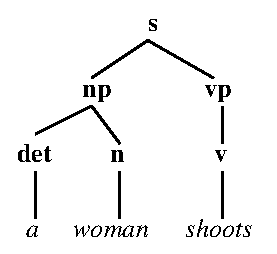
\includegraphics{parse2.eps}  
we could have the following term:  
\begin{LPNcodedisplay}
s(np(det(a),n(woman)),vp(v(shoots))).
\end{LPNcodedisplay}
Sure: it doesn't \LPNemph{look} as nice, but all the information in   
the picture is there.  And, with the aid of a decent graphics package,   
it would be easy to turn this term into a picture.

But how do we get DCGs to build such terms?  Actually, it's pretty   
easy.  After all, in effect a DCG has to work out what the tree   
structure is when recognising a sentence.  So we just need to find a   
way of keeping track of the structure that the DCG finds.  We do this   
by adding extra arguments.  Here's how:  
\begin{LPNcodedisplay}
s(s(NP,VP)) --> np(NP),vp(VP).

np(np(DET,N)) --> det(DET),n(N).

vp(vp(V,NP)) --> v(V),np(NP).
vp(vp(V))    --> v(V).

det(det(the)) --> [the].
det(det(a))   --> [a].

n(n(woman)) --> [woman].
n(n(man))   --> [man].

v(v(shoots)) --> [shoots].
\end{LPNcodedisplay}


What's going on here? Essentially we are building the parse trees for
the syntactic categories on the left hand side of the rules out of the
parse trees for the syntactic categories on the right hand side of the
rules. Consider the rule �vp(vp(V,NP)) --> v(V),np(NP)�.  When we make
a query using this DCG, the �V� in �v(V)� and the �NP� in �np(NP)�
will be instantiated to terms representing parse trees. For example,
perhaps �V� will be instantiated to
\begin{LPNcodedisplay}
v(shoots)
\end{LPNcodedisplay}
and �NP� will be instantiated to  
\begin{LPNcodedisplay}
np(det(a),n(woman)).
\end{LPNcodedisplay}
What is the term corresponding to a vp made out of these  
two structures? Obviously it should be this:  
\begin{LPNcodedisplay}
vp(v(shoots),np(det(a),n(woman))).
\end{LPNcodedisplay}
And this is precisely what the extra argument �vp(V,NP)� given in the
rule �vp(vp(V,NP)) -->� �v(V),np(NP)� returns to us:  a term
whose functor is �vp�, and whose first and second arguments are the
values of �V� and �NP� respectively. To put it informally: it plugs
the �V� and the �NP� terms together under a �vp� functor.

To parse the sentence ``A woman shoots'' we pose the query:  
\begin{LPNcodedisplay}
?- s(T,[a,woman,shoots],[]).
\end{LPNcodedisplay}
That is, we ask for the extra argument �T� to be instantiated   
to a parse tree for the sentence.  And we get:  
\begin{LPNcodedisplay}
T = s(np(det(a),n(woman)),vp(v(shoots))) 
yes
\end{LPNcodedisplay}
  
Furthermore, we can generate all parse trees by making the following   
query:  
\begin{LPNcodedisplay}
?- s(T,S,[]).
\end{LPNcodedisplay}
The first three responses are:  
\begin{LPNcodedisplay}
T = s(np(det(the),n(woman)),
      vp(v(shoots),np(det(the),n(woman)))) 
S = [the,woman,shoots,the,woman] ;

T = s(np(det(the),n(woman)),
      vp(v(shoots),np(det(the),n(man)))) 
S = [the,woman,shoots,the,man] ;

T = s(np(det(the),n(woman)),
      vp(v(shoots),np(det(a),n(woman)))) 
S = [the,woman,shoots,a,woman] 
\end{LPNcodedisplay}
In short, we have just seen an elegant (and useful) example of how to
build structure using unification.

Extra arguments can also be used to build \LPNterm{semantic
representations}.  Now, we did not say anything about what the words
in our little DCG mean.  In fact, nowadays a lot is known about the
semantics of natural languages, and it is surprisingly easy to build
semantic representations which partially capture the meaning of
sentences or even entire discourses.  Such representations are usually
expressions of some formal language (for example first-order logic,
discourse representation structures, or a database query language) and
they are usually built up \LPNterm{compositio\-nally}.  That is, the
meaning of each word is expressed in the formal language; this meaning
is given as an extra argument in the DCG entries for the individual
words.  Then, for each rule in the grammar, an extra argument shows
how to combine the meaning of the two subcomponents.  For example, to
the rule �s --> np, vp� we would add an extra argument stating how to
combine the �np� meaning and the �vp� meaning to form the �s� meaning.
Although somewhat more complex, the semantic construction process is
quite like the way we built up the parse tree for the sentence from
the parse tree of its subparts.%
\footnote{For a detailed account of how to do this, see
\textit{Representation and Inference for Natural Language: A First
Course in Computational Semantics}, Patrick Blackburn and Johan Bos,
CSLI Publications, 2005.}


\subsection*{Beyond context free languages}\label{SUBSEC.L8.NON.CONTEXT.FREE}



In the previous chapter we introduced DCGs as a useful Prolog tool for  
representing and working with context free grammars. Now, this is  
certainly a good way of thinking about DCGs, but it's not the whole  
story. For the fact of the matter is: DCGs can deal with a lot more  
than just context free languages. The extra arguments we have been  
discussing (and indeed, the extra goals we shall introduce shortly)  
give us the tools for coping with any computable language  
whatsoever. We shall illustrate this by presenting a simple DCG for the  
formal language $a^nb^nc^n \backslash \{ \epsilon \}$.

The formal language $a^nb^nc^n \backslash \{ \epsilon \}$  consists
of all non-null strings made up of �a�s, �b�s, and �c�s which consist
of an unbroken block of �a�s, followed by an unbroken block of �b�s,
followed by an unbroken block of �c�s, all three blocks having the
same length. For example, �abc�, and �aabbcc� and �aaabbbccc� all
belong to 
$a^nb^nc^n \backslash \{ \epsilon \}$.

The interesting thing about this language is that it is \LPNemph{not}  
context free. Try whatever you like, you will not succeed in writing a  
context free grammar that generates precisely these strings. Proving  
this would take us too far afield, but the proof is not particularly  
difficult, and you can find it in many books on formal language  
theory.

 On the other hand, as we shall now see, it is very easy to write a
DCG that generates this language. Just as we did in the previous
chapter, we shall represent strings as lists; for example, the string
�abc� will be represented using the list �[a,b,c]�. Given this
convention, here's the DCG we need:
\begin{LPNcodedisplay}
s(Count) --> ablock(Count),bblock(Count),cblock(Count).

ablock(0) --> [].
ablock(succ(Count)) --> [a],ablock(Count).

bblock(0) --> [].
bblock(succ(Count)) --> [b],bblock(Count).

cblock(0) --> [].
cblock(succ(Count)) --> [c],cblock(Count).
\end{LPNcodedisplay}


The idea underlying this DCG is fairly simple: we use an extra  
argument to keep track of the length of the blocks. The �s� rule  
simply says that we want a block of �a�s followed by a block of  
�b�s followed by block of �c�s, and all three blocks are to  
have the same length, namely �Count�.

What should the values of �Count� be? The obvious answer is: �1�, �2�,
�3�, �4�, and so on.  But as yet we don't know how to mix DCGs and
arithmetic, so this isn't very helpful. Fortunately, as this DCG
shows, there's an easier (and more elegant) way. Represent the
number 0 by �0�, the number 1 by �succ(0)�, the number 2 by
�succ(succ(0))�, the number 3 by �succ(succ(succ(0)))�, and so on,
just as we did it in Chapter~3 (as we said in Chapter~3, you can read
�succ� as ``successor of'').  This choice of notation
enables us to count using unification.

And this is precisely what our new  DCG does.
For example, suppose we pose the following query:  
\begin{LPNcodedisplay}
?- s(Count,L,[]).
\end{LPNcodedisplay}
which asks Prolog to generate the lists �L� of symbols that  
belong to this language, and to give the value of �Count� needed  
to produce each item. Then the first four responses are:  
\begin{LPNcodedisplay}
Count = 0
L = [] ;

Count = succ(0)
L = [a, b, c] ;
 
Count = succ(succ(0))
L = [a, a, b, b, c, c] ;
 
Count = succ(succ(succ(0)))
L = [a, a, a, b, b, b, c, c, c]
\end{LPNcodedisplay}
  
The value of �Count� clearly corresponds to the  
length of the blocks.

 So: DCGs are not just a tool for working with context free  
grammars. They are strictly more powerful than that, and (as we've  
just seen) part of the extra power comes from the use of extra  
arguments.

\section{Extra Goals}\label{SEC.L8.TESTS}



Any DCG rule is really syntactic sugar for an ordinary Prolog rule.
So it's not really too surprising that we're allowed to make use of
extra arguments.  Similarly, it shouldn't come as too much of a
surprise that we can call any Prolog predicate whatsoever from the
right hand side of a DCG rule.

The DCG of the previous section can, for example, be adapted to work
with Prolog numbers (instead of the successor representation of
numbers) by using calls to Prolog's built-in arithmetic
functionality. We simply count how many �a�s, �b�s, and �c�s have been
generated. Here's the code:
\begin{LPNcodedisplay}
s --> ablock(Count),bblock(Count),cblock(Count).

ablock(0) --> [].
ablock(NewCount) --> [a],ablock(Count), 
                     {NewCount is Count + 1}.

bblock(0) --> [].
bblock(NewCount) --> [b],bblock(Count), 
                     {NewCount is Count + 1}.

cblock(0) --> [].
cblock(NewCount) --> [c],cblock(Count),      
                     {NewCount is Count + 1}.
\end{LPNcodedisplay}
  
As this example suggests, extra goals can be written (anywhere) on the
right side of a DCG rule, but must be placed between curly
brackets. When Prolog encounters such curly brackets while translating
a DCG into its internal representation, it just takes the extra goals
specified between the curly brackets over into the translation. So,
the second rule for the non-terminal �ablock� above would be
translated as follows:
\begin{LPNcodedisplay}
ablock(NewCount,A,B):- 
   'C'(A, a, C),
   ablock(Count, C, B),
   NewCount is Count + 1. 
\end{LPNcodedisplay}


Incidentally, if you play around with this DCG, you will find that
there are actually some problems with it. In contrast to the one that
we saw in the last section, this new version only works correctly when
used in the recognition mode. If you try to generate with it, it will
at some point enter an infinite loop. We won't bother to fix this
problem here (apart from anything else, we find the earlier �succ�
based approach more elegant).

The possibility of adding arbitrary Prolog goals to the right hand
side of DCG rules, makes DCGs very powerful (it means that we can do
anything that we can do in plain Prolog). In general, however, this
capability is not used much, which tends to suggest that the basic DCG
notation is well designed.  There is, however, one classic application
for extra goals in computational linguistics: with the help of extra
goals, we can neatly separate grammar rules and lexical
information. Let's see how.

\subsection*{Separating rules and lexicon}\label{SUBSEC.L8.SEP.RULE.LEX}


We are going to separate rules and lexicon. That is, we are going to
eliminate all mention of individual words in our DCGs and instead
record all the information about individual words separately in a
lexicon.  To see what is meant by this, let's return to our basic
grammar:
\begin{LPNcodedisplay}
np --> det,n.

vp --> v,np.
vp --> v.

det --> [the].
det --> [a].

n --> [woman].
n --> [man].

v --> [shoots].  
\end{LPNcodedisplay}
We are now going to write a DCG that generates exactly  
the same language, but in which no rule mentions any individual  
word. All the information about individual words will be recorded  
separately. 

   
Here is an example of a (very simple) lexicon. Lexical entries are  
encoded by using a predicate �lex/2� whose first argument is a  
word, and whose second argument is a syntactic category.  
\begin{LPNcodedisplay}
lex(the,det).
lex(a,det).
lex(woman,n).
lex(man,n).
lex(shoots,v).
\end{LPNcodedisplay}

And here is a simple grammar that could go with this lexicon.  In
essence it's the same as the previous one.  In fact, the only rules
that have changed are those that mentioned specific words, that is,
the �det�, �n�, and �v� rules.
\begin{LPNcodedisplay}
np --> det,n.

vp --> v,np.
vp --> v.

det --> [Word],{lex(Word,det)}.
n --> [Word],{lex(Word,n)}.
v --> [Word],{lex(Word,v)}.
\end{LPNcodedisplay}
  
Consider the new �det� rule. This rule part says ``a �det�  
can consist of a list containing a single element �Word�'' (note  
that �Word� is a variable). Then the extra goal adds the crucial  
stipulation: ``so long as �Word� unifies  with something that is  
listed in the lexicon as a determiner''.  With our present lexicon,  
this means that �Word� must be matched either with the word ``a''  
or ``the''.  So this single rule replaces the two previous DCG rules  
for �det�.

This explains the ``how'' of separating rules from lexicon, but it  
doesn't explain the ``why''. Is it really so important? Is this new  
way of writing DCGs really that much better?

The answer is an unequivocal yes! It's \LPNemph{much} better, and for  
at least two reasons.

The first reason is theoretical. Arguably rules should not mention
specific lexical items. The purpose of rules is to list
\LPNemph{general} syntactic facts, such as the fact that sentence can
be made up of a noun phrase followed by a verb phrase. The rules for
�s�, �np�, and �vp� describe such general syntactic facts, but the old
rules for �det�, �n�, and �v� don't. Instead, the old rules simply
list particular facts: that ``a'' is a determiner, that ``the'' is a
determiner, and so on.  From theoretical perspective it is much neater
to have a single rule that says ``anything is a determiner (or a noun,
or a verb, or any other grammatical category) if it is listed as such
in the lexicon''. And this, of course, is precisely what our new DCG
rules say.

The second reason is more practical. One of the key lessons  
computational linguists have learnt over the last twenty or so years  
is that the lexicon is by far the most interesting, important (and  
expensive!) repository of linguistic knowledge. Bluntly, if you want  
to get to grips with natural language from a computational perspective,  
you need to know a lot of words, and you need to know a lot about them.

 Now, our little lexicon, with its simple two-place �lex� entries, is
a toy. But a real lexicon is (most emphatically!) not. A real lexicon
is likely to be very large (it may contain hundreds of thousands of
words) and moreover, the information associated with each word is
likely to be very rich.  Our �lex� entries give only the syntactical
category of each word, but a real lexicon will give much more, such as
information about its phonological, morphological, semantic, and
pragmatic properties.

Because real lexicons are big and complex, from a software engineering  
perspective it is best to write simple grammars that have a simple,  
well-defined way, of pulling out the information they need from vast  
lexicons. That is, grammars should be thought of as separate entities  
which can access the information contained in lexicons. We can then  
use specialised mechanisms for efficiently storing the lexicon and  
retrieving data from it. 

Our new DCG rules, though simple, illustrate the basic idea. The new
rules really do just list general syntactic facts, and the extra goals
act as an interface to our lexicon that lets the rules find exactly
the information they need. Furthermore, we now take advantage of
Prolog's 
\LPNterm{first argument indexing} which makes looking up a word in the
lexicon more efficient. First argument indexing is a technique for
making Prolog's knowledge base access more efficient. If in the query
the first argument is instantiated it allows Prolog to ignore all
clauses where the first argument's functor and arity is
different. This means, for example, that we can get all the possible
categories of �man� immediately without having to even look at the
lexicon entries for all the other hundreds or thousands of words that
we might have in our lexicon.

\section{Concluding Remarks}\label{SEC.L8.CONCLUDING.REMARKS}



We now have a fairly useful picture of what DCGs are and what they can   
do for us.  To conclude, let's think about them from a somewhat higher   
level, from both a formal and a linguistic perspective.

First the formal remarks.  For the most part, we have presented DCGs
as a simple tool for encoding context free grammars (or context free
grammars enriched with features such as \LPNemph{subject} and
\LPNemph{object}).  But DCGs go beyond this.  We saw that it was
possible to write a DCG that generated a language that was not context
free.  In fact, \LPNemph{any program whatsoever} can be written in DCG
notation.  That is, DCGs are a full-fledged programming language in
their own right (they are Turing-complete, to use the proper
terminology).  And although DCGs are usually associated with
linguistic applications, they can be useful for other purposes.

How good are DCGs from a linguistic perspective?  Well, mixed.  At   
one stage (in the early 1980s) they were pretty much state of the art.    
They made it possible to code complex grammars in a clear way, and to   
explore the interplay of syntactic and semantic ideas.  Certainly any   
history of parsing in computational linguistics would give DCGs an   
honourable mention.

Nonetheless, DCGs have drawbacks.  For a start, their tendency to loop
when the goal ordering is wrong (we saw an example in the previous
chapter when we added a left-recursive rule for conjunctions) is
annoying; we \LPNemph{don't} want to think about such issues when
writing serious grammars. Furthermore, while the ability to add extra
arguments is useful, if we need to use lots of them (and for big
grammars we will) it is a rather clumsy mechanism.

It is important to notice, however, that these problems come up
because of the way Prolog interprets DCG rules. They are not inherent
to the DCG notation. Any of you who have studied parsing algorithms
probably know that all top-down parsers loop on left-recursive
grammars. So, it is not surprising that Prolog, which interprets DCGs
in a top-down fashion, loops on the left-recursive grammar rule 
�s --> s conj s�. If we used a different strategy to interpret DCGs, for
example a bottom-up strategy, we would not run into the same
problem. Similarly, if we didn't use Prolog's built-in interpretation
of DCGs, we could use the extra arguments for a more sophisticated
specification of features, one that would facilitate the use of large
feature structures.

Summing up, nowadays DCGs are probably best viewed as a nice notation
for defining context free grammars enhanced with some features, a
notation that (ignoring left-recursion) doubles as a
parser/recogniser.  That is, they are best viewed as a convenient tool
for testing new grammatical ideas, or for implementing reasonably
complex grammars for particular applications.  DCGs are no longer
state of the art, but they are useful.  Even if you have never
programmed before, simply by using what you have learned so far you
are ready to start experimenting with reasonably sophisticated grammar
writing.  With a conventional programming language (such as C++ or
Java) it simply wouldn't be possible to reach this stage so soon.
Things would be easier in functional languages (such as Lisp, Caml, or
Haskell), but even so, it is doubtful whether beginners could do so
much so early.

\section{Exercises}\label{SEC.L8.EXERCISES}

\begin{LPNexercise}{L8.EX1} Here's our basic DCG:  
\begin{LPNcodedisplay}
s --> np,vp.

np --> det,n.

vp --> v,np.
vp --> v.

det --> [the].
det --> [a].

n --> [woman].
n --> [man].
n --> [apple].
n --> [pear].

v --> [eats].
\end{LPNcodedisplay}
  
  
Suppose we add the noun ``men'' (which is plural) and the verb  
``know''.  Then we would want a DCG which says that ``The men eat''  
is ok, ``The man eats'' is ok, ``The men eats'' is not ok, and  
``The man eat'' is not ok. Change the DCG so that it correctly  
handles these sentences. Use an extra argument to cope with the  
singular/plural distinction.
\end{LPNexercise}



\begin{LPNexercise}{L8.EX2}
In the text, we only gave examples of DCG rules
with one extra argument, but in fact you can add as many extra
arguments as you like. Here's a DCG rule
with three extra arguments:
\begin{LPNcodedisplay}
kanga(V,R,Q) --> roo(V,R),jumps(Q,Q),{marsupial(V,R,Q)}.
\end{LPNcodedisplay}
Translate it into the form Prolog uses.
\end{LPNexercise}

\section{Practical Session}\label{SEC.L8.PRAXIS}



The purpose of Practical Session 8 is to help you get familiar with  
DCGs that make use of additional arguments and goals.

First some keyboard exercises:  
\begin{enumerate}
\item{}Trace some examples using the DCG which uses extra arguments to  
handle the subject/object distinction, the DCG which produces parses, and  
the DCG which uses extra goals to separate lexicon and rules. Make sure  
you fully understand the way all three DCGs work.

\item{}Carry out traces on the DCG for $a^nb^nc^n$ given in the text
(the one that gave the �Count� variable the values �0�, �succ(0)�,
�succ(succ(0))�, and so on). Try cases where the three blocks of �a�s,
�b�s, and �c�s are indeed of the same length as well as queries where
this is not the case.
\end{enumerate}

Now for some programming. We suggest the following mini-project, which
draws on all you have learned so far. Incidentally, in the Practical
Session at the end of Chapter~12 we will be asking to extend this work
even further, so do take this project seriously.
\begin{enumerate}
\item{}First, bring together all the things we have learned about DCGs
for English into one DCG. In particular, in the text we saw how to use
extra arguments to deal with the subject/object distinction, and in
the exercises you were asked to use additional arguments to deal with
the singular/plural distinction. Write a DCG which handles
both. Moreover, write the DCG in such a way that it will produce parse
trees, and makes use of a separate lexicon.
\item{}Once you have done this, extend the DCG so that noun phrases can  
be modified by adjectives and simple prepositional phrases (that is,  
it should be able to handle noun phrases such as ``the small  
frightened woman on the table'' or ``the big fat cow under the  
shower''). Then, further extend it so that the distinction between  
first, second, and third person pronouns is correctly handled (both in  
subject and object form).
\end{enumerate}



\chapter{A Closer Look at Terms}\label{CHAPTER9}

\Thischapter{115}{

\noindent
This chapter has three main goals:  
  
\begin{enumerate}

\item{}To introduce the \texttt{==} predicate.

\item{}To take a closer look at term structure.

\item{}To introduce operators.

\end{enumerate}

}

\section{Comparing Terms}\label{SEC.L9.COMPARING.TERMS}



Prolog contains an important predicate for comparing terms, namely the
\LPNterm{identity predicate} �==/2�. As its name suggests, this tests
whether two terms are identical.  However �==/2� does \LPNemph{not}
instantiate variables, thus it is not the same as the unification
predicate �=/2�.\index{PROLOG ==/2@\texttt{==/2}} Let's look at some
examples.
\begin{LPNcodedisplay}
?- a == a.
yes

?- a == b.
no

?- a == 'a'.
yes
\end{LPNcodedisplay}
The reason Prolog gives these answers should be clear, though pay
attention to the last one.  It tells us that, as far as Prolog is
concerned, �a� and �'a'� are the same object.

Now let's look at examples involving variables, and explicitly compare   
�==� with the unification predicate �=�.  
  
\begin{LPNcodedisplay}
?- X==Y.
no

?- X=Y.
X = _2808 
Y = _2808 
yes
\end{LPNcodedisplay}
In these queries, �X� and �Y� are \LPNemph{uninstantiated}   
variables; we haven't given them any value.  Thus the first answer is   
correct: �X� and �Y� are \LPNemph{not} identical objects, so the   
�==� test fails.  On the other hand, the use of �=� succeeds,   
for �X� and �Y� can be unified.

Let's now look at queries involving \LPNemph{instantiated} variables:  
\begin{LPNcodedisplay}
?- a=X, a==X.

X = a 
yes
\end{LPNcodedisplay}
The first conjunct, �a=X�, binds �X� to �a�.  Thus when   
�a==X� is evaluated, the left hand side and right hand sides are   
exactly the same Prolog object, and �a==X� succeeds.

A similar thing happens in the following query:   
\begin{LPNcodedisplay}
?- X=Y, X==Y.

X = _4500 
Y = _4500 
yes
\end{LPNcodedisplay}
The conjunct �X=Y� first unifies the variables �X� and �Y�.  Thus when
the second conjunct �X==Y� is evaluated, the two variables are exactly
the same Prolog object, and the second conjunct succeeds as well.

It should now be clear that �=� and �==� are different, nonetheless
there is an important relation between them: �==� can be viewed as a
stronger test for equality between terms than �=�.  That is, if
�term1� and �term� are Prolog terms, and the query �term1 == term2�
succeeds, then the query �term1 = term2� will succeed too.

Another predicate worth knowing about is �\==�.  This predicate is
defined so that it succeeds in precisely those cases where �==� fails.
That is, it succeeds whenever two terms are \LPNemph{not}\index{PROLOG
\==/2@\verb-\==/2-} identical, and fails otherwise.  For example:
\begin{LPNcodedisplay}
?- a \== a.
no

?- a \== b.
yes

?- a \== 'a'.
no
\end{LPNcodedisplay}
These answers should be understandable: they are simply the opposite of the
answers we got above when we used �==�. Now consider:
\begin{LPNcodedisplay}
?- X \== a.

X = _3719 
yes
\end{LPNcodedisplay}
Why this response?  Well, we know from above that the query �X==a�
\LPNemph{fails} (recall the way �==� treats uninstantiated variables).
Thus the query �X\==a� should \LPNemph{succeed}, and it does.

Similarly:  
\begin{LPNcodedisplay}
?- X \== Y.

X = _798 
Y = _799 
yes
\end{LPNcodedisplay}
Again, we know from above that the query �X==Y� fails, thus the query
�X\==Y� succeeds.

\section{Terms with a Special Notation}\label{SEC.L9.SPECIAL.NOTATION}



Sometimes terms look different to us, but Prolog regards them as
identical.  For example, when we compare �a� and �'a'�, we see two
distinct strings of symbols, but Prolog treats them as the same.  And
in fact there are many other cases where Prolog regards two strings as
being exactly the same term.  Why?  Because it makes programming more
pleasant.  Sometimes the notation Prolog likes isn't as user-friendly
as the notation we would choose.  So it is nice to be able to write
programs in the notation we find natural, and to let Prolog run them
in the notation it prefers.

\subsection*{Arithmetic terms}\label{SUBSEC.L9.ARITHMETIC.TERMS}



The arithmetic predicates introduced earlier are a good example of
this.  As was mentioned in Chapter~\ref{CHAPTER5}, �+�, �-�, �*�, and
�/� are \LPNemph{functors}, and arithmetic expressions such as � 2+3�
are \LPNemph{terms}.  And this is not an analogy.  Apart from the fact
that it can evaluate them with the help of the �is/2� predicate,
Prolog views strings of symbols such as �2+3� as being identical with
ordinary complex terms. The following queries make this clear:
\begin{LPNcodedisplay}
?- 2+3 == +(2,3).
yes

?- +(2,3) == 2+3.
yes

?- 2-3 == -(2,3).
yes

?- *(2,3) == 2*3.
yes

?- 2*(7+2) == *(2,+(7,2)).
yes
\end{LPNcodedisplay}
In short, the familiar arithmetic notation is there for \LPNemph{our}   
convenience.  Prolog doesn't regard it as different from the usual   
term notation.

Similar remarks to the arithmetic comparison predicates �<�, �=<�, �=:=�, �=\=�, �>� and �>=�:  
\begin{LPNcodedisplay}
?- (2 < 3) == <(2,3).
yes

?- (2 =< 3) == =<(2,3).
yes

?- (2 =:= 3) == =:=(2,3).
yes

?- (2 =\= 3) == =\=(2,3).
yes

?- (2 > 3) == >(2,3).
yes

?- (2 >= 3) == >=(2,3).
yes
\end{LPNcodedisplay}

These example show why it's nice to have the user-friendly notation
(would you want to have to work with expressions like
�=:=(2,3)�?). Note, by the way, that we enclosed the left hand
arguments in brackets. For example, we didn't ask
\begin{LPNcodedisplay}
?- 2 =:= 3 == =:=(2,3).
\end{LPNcodedisplay}
we asked  
\begin{LPNcodedisplay}
?- (2 =:= 3) == =:=(2,3).
\end{LPNcodedisplay}
Why?  Well, Prolog finds the query �2 =:= 3 == =:=(2,3)� confusing,
and let's face it,  can you blame it?  It's not sure whether to bracket
this expression as �(2 =:= 3) == =:=(2,3)� (which is what we want), or
as �2 =:= (3 == =:=(2,3))�.  So we need to state the grouping
explicitly.

One final remark.  We have now introduced three rather similar looking   
symbols, namely �=�, �==�, and �=:=� (and indeed, there are  
also �\=�, �\==�, and �=\=�).  Here's a summary:  
  
\begin{center}\begin{tabular}{ll}
�=�&The unification predicate.\\
\strut&Succeeds if it can   
        unify its arguments, fails otherwise.\\
�\=�&The negation of the  unification predicate.\\
\strut&Succeeds if �=� fails, and vice-versa.\\
�==�&The identity predicate.\\
\strut&Succeeds if its arguments   
        are identical, fails otherwise.\\
�\==�&The negation of the  identity predicate.\\
\strut&Succeeds if �==� fails, and vice-versa.\\
�=:=�&The arithmetic equality predicate.\\
\strut&Succeeds if its arguments evaluate to the same integer.\\
�=\=�&The arithmetic inequality predicate.\\
\strut&Succeeds if its   
arguments evaluate to different integers.
\end{tabular}\end{center}



\subsection*{Lists as terms}\label{SUBSEC.L9.LIST.TERMS}



Lists are another good example of Prolog working with one internal
representation, while giving us another, more user-friendly, notation
to work with.  Let's start with a quick look at the user-friendly list
notation it provides (that is, the square brackets �[� and �]�).  In
fact, because Prolog also offers the �|� constructor, there are 
many ways of writing the same list, even at the user-friendly level:
  
\begin{LPNcodedisplay}
?- [a,b,c,d] == [a|[b,c,d]].
yes

?- [a,b,c,d] == [a,b|[c,d]].
yes

?- [a,b,c,d] == [a,b,c|[d]].
yes

?- [a,b,c,d] == [a,b,c,d|[]]. 
yes
\end{LPNcodedisplay}
  
  
  
But how does Prolog view lists internally?  In fact, it sees lists as
terms which are built out of two special terms, namely �[]�, which
represents the empty list, and ``�.�'' (the full-stop), a functor
of\index{PROLOG ./2@\texttt{./2}} arity 2 which is used to build
non-empty lists. The terms �[]� and �.� are called \LPNterm{list
constructors}.

This is how these constructors are used to build lists.  Needless to
say, the definition is recursive:
  
\begin{itemize}
\item{}The empty list is the term $[ \ ]$. It 
        has length 0.
\item{}A non-empty list is any term of the form $.(\textit{term},\textit{list})$,   
        where \textit{term} is any Prolog term, and \textit{list} is any   
        list.  If \textit{list} has length $n$, then $.(\textit{term},\textit{list})$ has 
        length $n+1$.
\end{itemize}

Let's make sure we fully understand this definition by working our way
through a few examples.
  
  
\begin{LPNcodedisplay}
?- .(a,[]) == [a].
yes

?- .(f(d,e),[]) == [f(d,e)].
yes

?- .(a,.(b,[])) == [a,b].
yes

?- .(a,.(b,.(f(d,e),[]))) == [a,b,f(d,e)].
yes

?- .(.(a,[]),[]) == [[a]].
yes

?- .(.(.(a,[]),[]),[]) == [[[a]]].
yes

?- .(.(a,.(b,[])),[]) == [[a,b]].
yes

?- .(.(a,.(b,[])),.(c,[])) == [[a,b],c].
yes

?- .(.(a,[]),.(b,.(c,[]))) == [[a],b,c].
yes

?- .(.(a,[]),.(.(b,.(c,[])),[])) == [[a],[b,c]].
yes
\end{LPNcodedisplay}
  
  
Prolog's internal notation for lists is not as user-friendly as the
use of the square bracket notation.  But it's not as bad as it seems
at first sight. In fact, it works similarly to the �|� notation. It
represents a list in two parts: its first element (the head), and a
list representing the rest of the list (the tail).  The trick is to
read these terms as \LPNemph{trees}. The internal nodes of this tree
are labeled with �.� and all have two daughter nodes.  The subtree
under the left daughter represents the first element of the list and
the subtree under the right daughter represents the rest of the list.
For example, the tree representation of
�.(a,.(.(b,.(c,[])),.(d,[])))�, that is, �[a, [b,c], d]�, looks like
this:
  
\begin{center}
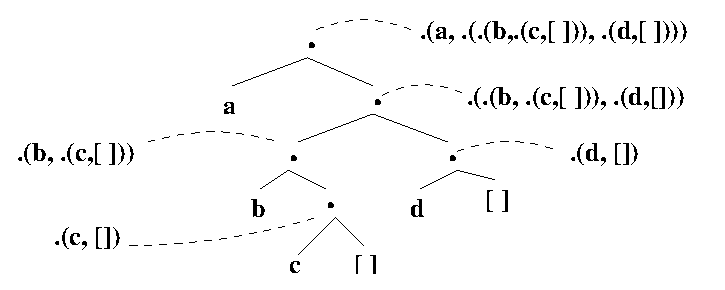
\includegraphics[scale=.7]{listtree.eps}  
\end{center}

  
One final remark. Prolog is very polite. Not only are you free to talk
to it in the user-friendly notation, it will reply in the same way:
\begin{LPNcodedisplay}
?- .(f(d,e),[]) = Y.

Y = [f(d,e)] 
yes


?- .(a,.(b,[])) = X, Z= .(.(c,[]),[]), W = [1,2,X].

X = [a,b] 
Z = [[c]] 
W = [1,2,[a,b]] 
yes
\end{LPNcodedisplay}


\section{Examining Terms}\label{SEC.L9.EXAMINING}



In this section, we will learn about some built-in predicates that let
us examine terms more closely. First, we will look at predicates that
test whether their arguments are terms of a certain type (for example,
whether they are atoms or numbers). Then we will introduce predicates
that tell us something about the internal structure of complex terms.


\subsection*{Types of Terms}\label{SUBSEC.L9.TERMTYPES}

Remember what we said about Prolog terms in Chapter~\ref{CHAPTER1}:
there are four different kinds, namely variables, atoms, numbers and
complex terms.  Furthermore, atoms and numbers are grouped together
under the name constants, and constants and variables constitute the
simple terms. The following tree diagram summarises this:
 
\begin{center} 
  \pstree[levelsep=10mm,nodesep=2mm]{\TR{terms}}
    { \pstree[levelsep=10mm,nodesep=2mm]{\TR{simple terms}}
         { \TR{variables}
           \pstree[levelsep=10mm,nodesep=2mm]{\TR{constants}}
               { \TR{atoms}
                 \TR{numbers} }}
      \TR{complex terms} }

%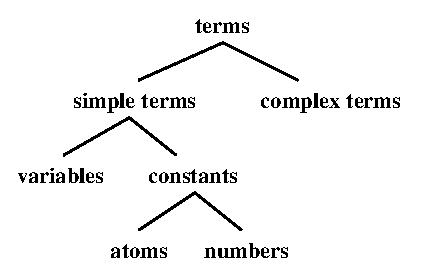
\includegraphics{termtypes.eps}  
\end{center}
  
Sometimes it is useful to be able to determine what type a given term
is. You might, for example, want to write a predicate that has to deal
with different kinds of terms, but has to treat them in different
ways.  Prolog provides several built-in predicates that test whether a
given term is of a certain type:
  
\begin{center}\begin{tabular}{ll}
�atom/1�&Is the argument an atom?\\ \index{PROLOG atom/1@\texttt{atom/1}}
�integer/1�&Is  the argument  an integer?\\ \index{PROLOG integer/1@\texttt{integer/1}}
�float/1�&Is the argument a floating point number?\\ \index{PROLOG float/1@\texttt{float/1}}
�number/1�&Is  the argument an integer or a floating point number?\\ \index{PROLOG number/1@\texttt{number/1}}
�atomic/1�&Is the  argument a constant?\\ \index{PROLOG atomic/1@\texttt{atomic/1}}
�var/1�&Is the argument an uninstantiated variable?\\ \index{PROLOG var/1@\texttt{var/1}}
�nonvar/1�&\parbox[t]{0.75\textwidth}{Is  the argument an instantiated variable or another term that is not an \LPNemph{un}instantiated variable?} \index{PROLOG nonvar/1@\texttt{nonvar/1}}
\end{tabular}\end{center}  

  
Let's see how they behave.  
  
\begin{LPNcodedisplay}
?- atom(a).
yes

?- atom(7).
no

?- atom(loves(vincent,mia)).
no
\end{LPNcodedisplay}
These three examples behave exactly as we would expect.  But what
happens, when we call �atom/1� with a variable as argument?
\begin{LPNcodedisplay}
?- atom(X).
no
\end{LPNcodedisplay}
This makes sense, since an uninstantiated variable is not an atom.
However if we instantiate �X� with an atom first and then ask
�atom(X)�, Prolog answers yes.
\begin{LPNcodedisplay}
?- X = a, atom(X).
X = a
yes
\end{LPNcodedisplay}
But it is important that the instantiation is done \LPNemph{before} the  
test:   
\begin{LPNcodedisplay}
?- atom(X), X = a.
no
\end{LPNcodedisplay}
The predicates �integer/1� and �float/1� behave analogously.  Try some
examples.

The predicates �number/1� and �atomic/1� behave disjunctively.  First,
�number/1� tests whether a given term is either an integer or a float:
that is, it will evaluate to true whenever either �integer/1� or
�float/1� evaluate to true and it fails when both of them fail.  As
for �atomic/1�, this tests whether a given term is a constant, that
is, whether it is either an atom or a number. So �atomic/1� will
evaluate to true whenever either �atom/1� or �number/1� evaluate to
true and it fails when both fail.
  
\begin{LPNcodedisplay}
?- atomic(mia).
yes

?- atomic(8).
yes

?- atomic(3.25).
yes

?- atomic(loves(vincent,mia)).
no

?- atomic(X)
no
\end{LPNcodedisplay}
  
What about variables?  First there is the �var/1� predicate. This
tests whether the argument is an \LPNemph{uninstantiated} variable:
\begin{LPNcodedisplay}
?- var(X)
yes

?- var(mia).
no

?- var(8).
no

?- var(3.25).
no

?- var(loves(vincent,mia)).
no
\end{LPNcodedisplay}

Then there is the �nonvar/1� predicate. This succeeds precisely when
�var/1� fails; that is, it tests whether its argument is \LPNemph{not}
an uninstantiated variable:
\begin{LPNcodedisplay}
?- nonvar(X)
no

?- nonvar(mia).
yes

?- nonvar(8).
yes

?- nonvar(3.25).
yes

?- nonvar(loves(vincent,mia)).
yes
\end{LPNcodedisplay}
  
Note that a complex term which contains uninstantiated variables is
not itself an uninstantiated variable (it is a  complex
term). Therefore we have:
  
\begin{LPNcodedisplay}
?- var(loves(_,mia)).
no

?- nonvar(loves(_,mia)).
yes
\end{LPNcodedisplay}
  
And  when the variable �X� gets instantiated �var(X)�  
and �nonvar(X)� behave differently depending on whether they are  
called before or after the instantiation: 
  
\begin{LPNcodedisplay}
?- X = a, var(X).
no 

?- X = a, nonvar(X).
X = a 
yes

?- var(X), X = a.
X = a
yes

?- nonvar(X), X = a.
no
\end{LPNcodedisplay}




\subsection*{The Structure of Terms}\label{SUBSEC.L9.TERMSTRUCTURE}

Given a complex term of unknown structure (perhaps a complex term
returned as the output of some predicate), what kind of information
might we want to extract from it? The obvious response is: its
functor, its arity, and what its arguments look like. Prolog
provides built-in predicates that provide this
information. Information about the functor\index{PROLOG
functor/3@\texttt{functor/3}} and arity is supplied by the predicate
�functor/3�.  Given a complex term, �functor/3� will tell us what its
functor and arity are:
  
\begin{LPNcodedisplay}
?- functor(f(a,b),F,A).
A = 2
F = f
yes

?- functor([a,b,c],X,Y).
X = '.'
Y = 2 
yes
\end{LPNcodedisplay}
Note that when asked about a list, Prolog returns the functor ., which
is the functor it uses in its internal representation of lists.

What happens when we use �functor/3� with constants? Let's try:
\begin{LPNcodedisplay}
?- functor(mia,F,A).
A = 0
F = mia
yes

?- functor(8,F,A).
A = 0
F = 8
yes

?- functor(3.25,F,A).
A = 0
F = 3.25
yes
\end{LPNcodedisplay}

So we can use the predicate �functor/3� to find out the functor and the
arity of a term, and this usage also works for the special case of 0
arity terms (constants). 

We can also use
�functor/3� to \LPNemph{construct} terms. How?
By specifying the second and third argument and leaving the first
undetermined.  The query
\begin{LPNcodedisplay}
?- functor(T,f,7).
\end{LPNcodedisplay}
for example, returns the following answer:  
\begin{LPNcodedisplay}
T = f(_G286, _G287, _G288, _G289, _G290, _G291, _G292)
yes
\end{LPNcodedisplay}
Note that either the first argument or the second and third argument
have to be instantiated. For example, Prolog would answer with an
error message to the query �functor(T,f,N)�. And if you think about
what the query means, Prolog is  reacting in a sensible
way. The query is asking Prolog to construct a complex term without
telling it how many arguments to provide, which is not a very sensible
request.

Now that we know about �functor/3�, let's put it to work.  In the
previous section, we discussed the built-in predicates that tested
whether their argument was an atom, a number, a constant, or a
variable. But there was no predicate that tested whether its argument
was a complex term.  To make the list complete, let's define such a
predicate. It is easy to do so using �functor/3�.  All we have to do
is to check that there is a suitable functor, and that the input has
arguments (that is, that its arity is greater than zero).  Here is the
definition:
  
\begin{LPNcodedisplay}
complexterm(X):-
   nonvar(X),
   functor(X,_,A),
   A > 0.
\end{LPNcodedisplay}

So much for functors --- what about arguments?  In addition to
the\index{PROLOG arg/3@\texttt{arg/3}} predicate �functor/3�, Prolog
supplies us with the predicate �arg/3� which tells us about the
arguments of complex terms. It takes a number \LPNemph{N} and a
complex term \LPNemph{T} and returns the \LPNemph{Nth} argument of
\LPNemph{T} in its third argument.  It can be used to access the value
of an argument
\begin{LPNcodedisplay}
?- arg(2,loves(vincent,mia),X).
X = mia
yes
\end{LPNcodedisplay}
or to instantiate an argument  
\begin{LPNcodedisplay}
?- arg(2,loves(vincent,X),mia).
X = mia
yes
\end{LPNcodedisplay}
Trying to access an argument which doesn't exist, of course, fails:  
\begin{LPNcodedisplay}
?- arg(2,happy(yolanda),X).
no
\end{LPNcodedisplay}

The predicates �functor/3� and �arg/3� allow us to access all the
basic information we need to know about complex terms. However Prolog
also supplies a third built-in predicate for analysing term structure,
namely �'=..'/2�. This takes a complex term and returns a list that
has the functor as its head, and then all the arguments, in order, as
the elements of the tail.  So to the query
\begin{LPNcodedisplay}
?- '=..'(loves(vincent,mia),X) 
\end{LPNcodedisplay}
Prolog will respond
\begin{LPNcodedisplay}
�X = [loves,vincent,mia]
\end{LPNcodedisplay}
This predicate (which is called \LPNterm{univ}) can also be used as an
infix operator. Here are some examples showing various ways of
using\index{PROLOG =..@\texttt{=../2}} this (very useful) tool:
\begin{LPNcodedisplay}
?- cause(vincent,dead(zed)) =.. X.
X = [cause, vincent, dead(zed)] 
yes

?- X =.. [a,b(c),d].
X = a(b(c), d) 
yes

?- footmassage(Y,mia) =.. X.
Y = _G303
X = [footmassage, _G303, mia] 
yes
\end{LPNcodedisplay}
  
Univ really comes into its own when something has to be done to all
arguments of a complex term. Since it returns the arguments as a list,
normal list processing strategies can be used to traverse the
arguments.  


\subsection*{Strings}\label{SUBSEC.L9.STRINGS}

Strings are represented in Prolog by a list of character (ASCII)
codes. However, it would be a right kerfuffle to use list notation for
simple string manipulation, so Prolog also offers a user-friendly
notation for strings: double quotes. Try the following query:

\begin{LPNcodedisplay}
?- S = "Vicky".
S = [86, 105, 99, 107, 121]
yes
\end{LPNcodedisplay}
Here the variable \texttt{S} unifies with the string \texttt{"Vicky"},
which is a list containing of five numbers, each of them corresponding
to the character codes of the single characters the strings is
composed of.  (For instance, 86 is the character code for the
character V, 105 is the code for the character i, and so on.)

In other words, strings in Prolog are actually lists of
numbers. Several standard predicates are supported by most Prolog
dialects to work with strings. A particularly useful one is
\texttt{atom\_codes/2}. This predicate converts an atom into a string. The
following examples illustrate what \texttt{atom\_codes/2}\index{PROLOG
atom\_codes/2@\texttt{atom\_codes/2}} can do for you:

\begin{LPNcodedisplay}
?- atom_codes(vicky,X).
X = [118, 105, 99, 107, 121]
yes

?- atom_codes('Vicky',X).
X = [86, 105, 99, 107, 121]
yes

?- atom_codes('Vicky Pollard',X).
X = [86, 105, 99, 107, 121, 32, 80, 111, 108|...]
yes
\end{LPNcodedisplay}

It also works the other way around: \texttt{atom\_codes/2} can also be used
to generate atoms from strings. Suppose you want to duplicate an atom
\texttt{abc} into the atom {abcabc}. This is how you could do it:

\begin{LPNcodedisplay}
?- atom_codes(abc,X), append(X,X,L), atom_codes(N,L).

X = [97, 98, 99]
L = [97, 98, 99, 97, 98, 99]
N = abcabc
\end{LPNcodedisplay}

One last thing you need to know about the \texttt{atom\_codes/2} predicate is
that it is related to another other built-in predicate, namely
\texttt{number\_codes/2}\index{PROLOG number\_codes/2@\texttt{number\_codes/2}}. 
This predicate behaves in a similar way, but, as the names suggest, only works for numbers.



\section{Operators}\label{SEC.L9.OPERATORS}


As we have seen, in certain cases (for example, when performing
arithmetic) Prolog lets us use operator notations that are more
user-friendly than its own internal representations.  Indeed, as we
shall now see, Prolog even has a mechanism for letting us define our
own operators.  In this section we'll first take a closer look at the
properties of operators, and then learn how to define our own.


\subsection*{Properties of operators}\label{SUBSEC.L9.OPERATORS.PROP}


Let's start with an example from arithmetic.  Internally, Prolog uses
the expression �is(11,+(2,*(3,3)))�, but we are free to write the
functors �*� and �+� between their arguments, to form the more 
user-friendly 
expression �11 is 2 + 3 * 3�.  Functors that can be written
between their arguments are called \LPNterm{infix operators}. Other
examples of infix operators in Prolog are �:-�, �-->�, �;�, �','�,
�=�, �=..�, �==� and so on.  In addition to infix operators there are
also \LPNterm{prefix operators} (which are written before their
arguments) and \LPNterm{postfix operators} (which are written after).
For example, �?-� is a prefix operator, and so is the one-place �-�
which is used to represent negative numbers (as in �1 is 3 + -2�). An
example of a postfix operator is the �++� notation used in the C
programming language to increment the value of a variable.

When we learned about arithmetic in Prolog, we saw that Prolog knows
about the conventions for disambiguating arithmetic expressions. So
when we write �2 + 3 * 3�, Prolog knows that we mean �2 + (3 * 3)� and
not �(2 + 3) * 3�. But how does Prolog know this? Because every
operator has a certain \LPNterm{precedence}. The precedence of �+� is
greater than the precedence of �*�, and that's why �+� is taken to be
the main functor of the expression �2 + 3 * 3�. (Note that Prolog's
internal representation �+(2,*(3,3))� is not ambiguous.)  Similarly,
the precedence of �is� is higher than the precedence of �+�, so 
�11 is 2 + 3 * 3� is interpreted as �is(11,+(2,*(3,3)))� and not as the
(nonsensical) expression �+(is(11,2),*(3,3))�.  In Prolog, precedence
is expressed by a number between 0 and 1200; the higher the number,
the greater the precedence.  To give some examples, the precedence of
�=� is 700, the precedence of �+� is 500, and the precedence of �*� is
400.


What happens when there are several operators with the same
precedence in one expression? We said above that Prolog finds the
query �2 =:= 3 == =:=(2,3)� confusing. It doesn't know how to
bracket the expression: Is it �=:=(2,==(3,=:=(2,3)))� or is it
�==(=:=(2,3),=:=(2,3))�? The reason Prolog is not able to decide on
the correct bracketing is because �==� and �=:=� have the same
precedence. In such cases, explicit bracketings must be supplied by
the programmer.

What about the following query though?  
\begin{LPNcodedisplay}
?- X is 2 + 3 + 4.
\end{LPNcodedisplay}
Does Prolog find this  confusing? Not at all: it deals with it happily
and correctly answers �X = 9�.  But which bracketing did Prolog
choose: �is(X,+(2,+(3,4)))� or �is(X,+(+(2,3),4))�? 
As the following queries show, it chose the second:
  
\begin{LPNcodedisplay}
?- 2 + 3 + 4 = +(2,+(3,4)).
no
?- 2 + 3 + 4 = +(+(2,3),4).
yes
\end{LPNcodedisplay}
  
  
Here Prolog has used information about the \LPNterm{associativity} of
�+�  to disambiguate:  �+� is \LPNterm{left
associative}, which means that the expression to the right of �+� must
have a lower precedence than �+� itself, whereas the expression on the
left may have the same precedence as �+�. The precedence of an
expression is simply the precedence of its main operator,  or 0 if it
is enclosed in brackets.  The main operator of �3 + 4� is �+�, so that
interpreting �2 + 3 + 4� as �+(2,+(3,4))� would mean that the
expression to the right of the first �+� has the same precedence as
�+� itself, which is illegal. It has to be lower.

The operators �==�, �=:=�, and �is� are defined to be  
\LPNterm{non-associative}, which means that both of their arguments must have  
a lower precedence. Therefore �2 =:= 3 == =:=(2,3)� is an illegal
expression,  
since no matter how you bracket it you'll get a conflict:  
�2 =:= 3� has the same precedence as �==�, and   
�3 == =:=(2,3)� has the same precedence as �=:=�.

The type of an operator (infix, prefix, or postfix), its precedence,
and its associativity are the three things that Prolog needs to know
to be able to translate user-friendly (but potentially ambiguous)
operator notations into Prolog's internal representation.



\subsection*{Defining operators}\label{SUBSEC.L9.OPERATORS.DEF}



In addition to providing a user-friendly operator notation for certain
functors, Prolog also lets you define your own operators. So you
could, for example, define a postfix operator �is_dead�; then
Prolog would allow you to write �zed is_dead� as a fact in your
database instead of �is_dead(zed)�.

Operator definitions in Prolog look like this:  \index{PROLOG op/3@\texttt{op/3}}
\begin{LPNcodedisplay}
:- op(Precedence,Type,Name).
\end{LPNcodedisplay}
As we mentioned above, precedence is a number between 0 and 1200, and
the higher the number, the greater the  precedence.  
Type is an
atom specifying the type and associativity of the operator. In the
case of �+� this atom is �yfx�, which says that �+� is an infix
operator; the �f� represents the operator,  and the �x� and �y� the
arguments.  Furthermore, �x� stands for an argument which has a
precedence which is lower than the precedence of �+� and �y� stands
for an argument which has a precedence which lower or equal to the
precedence of �+�.  There are the following possibilities for 
type:
\begin{center}\begin{tabular}{ll}
infix&�xfx�, �xfy�, �yfx�\\
prefix&�fx�, �fy�\\
suffix&�xf�, �yf�
\end{tabular}\end{center}  

So  your operator definition for �is_dead� might be as follows:  
\begin{LPNcodedisplay}
:- op(500, xf, is_dead).
\end{LPNcodedisplay}
  
  
Here are the definitions for some of the built-in operators. You can see  
that operators with the same properties can be specified in one statement  
by giving a list of their names (instead of a single name) as the third   
argument of �op�.  
  
\begin{center}\begin{tabular}{l}
�:- op( 1200, xfx, [ :-, --> ]).�\\
�:- op( 1200,  fx, [ :-, ?- ]).�\\
�:- op( 1100, xfy, [ ; ]).�\\
�:- op( 1000, xfy, [ ',' ]).�\\
�:- op(  700, xfx, [ =, is, =.., ==, \==, �\\
�                    =:=, =\=, <, >, =<, >= ]).�\\
�:- op(  500, yfx, [ +, -]).�\\
�:- op(  500,  fx, [ +, - ]).�\\
�:- op(  300, xfx, [ mod ]).�\\
�:- op(  200, xfy, [ ^ ]).�
\end{tabular}\end{center}

One final point should made explicit. Operator definitions don't
specify the \LPNemph{meanings} of operators, they only describe how
they can be used syntactically. That is, an operator definition
doesn't say anything about when a query involving this operator will
evaluate to true, it merely extends the \LPNemph{syntax} of
Prolog. So if the operator �is_dead� is defined as above, and you pose
the query �zed is_dead�, Prolog won't complain about illegal syntax
(as it would without this definition) but  will try to prove the
goal �is_dead(zed)�, which is Prolog's internal representation of 
�zed is_dead�. And this is all operator definitions do --- they just tell
Prolog how to translate a user-friendly notation into real Prolog
notation. So, what would be Prolog's answer to the query 
�zed is_dead�? It would be �no�, because Prolog would try to prove
�is_dead(zed)�, but would not find any matching clause in the
database.  But suppose we extended the database as follows:
\begin{LPNcodedisplay}
:- op(500, xf, is_dead).

kill(marsellus,zed).
is_dead(X) :- kill(_,X).
\end{LPNcodedisplay}
Now Prolog would answer �yes� to the query.   


\section{Exercises}\label{SEC.L9.EXERCISES}

\begin{LPNexercise}{L9.EX1}Which of the following queries succeed, and which fail?  
\begin{LPNcodedisplay}
?- 12 is 2*6.

?- 14 =\= 2*6.

?- 14 = 2*7.

?- 14 == 2*7.

?- 14 \== 2*7.

?- 14 =:= 2*7.

?- [1,2,3|[d,e]] == [1,2,3,d,e].

?- 2+3 == 3+2.

?- 2+3 =:= 3+2.

?- 7-2 =\= 9-2.

?- p == 'p'.

?- p =\= 'p'.

?- vincent == VAR.

?- vincent=VAR, VAR==vincent.

\end{LPNcodedisplay}
\end{LPNexercise}

\begin{LPNexercise}{L9.EX2}How does Prolog respond to the following queries?  
\begin{LPNcodedisplay}
?- .(a,.(b,.(c,[]))) = [a,b,c].

?- .(a,.(b,.(c,[]))) = [a,b|[c]].

?- .(.(a,[]),.(.(b,[]),.(.(c,[]),[]))) = X.

?- .(a,.(b,.(.(c,[]),[]))) = [a,b|[c]].
\end{LPNcodedisplay}
\end{LPNexercise}

\begin{LPNexercise}{L9.EX3}Write a two-place predicate �termtype(Term,Type)� that  
takes a term and gives back the type(s) of that term (atom, number,  
constant, variable, and so on). The types should be given back in the order  
of their generality. The predicate should  behave in the  
following way.   
\begin{LPNcodedisplay}
?- termtype(Vincent,variable).
yes
?- termtype(mia,X).
X = atom ;
X = constant ;
X = simple_term ;
X = term ;
no
?- termtype(dead(zed),X).
X = complex_term ;
X = term ;
no
\end{LPNcodedisplay}
\end{LPNexercise}


\begin{LPNexercise}{L9.EX4}Write a 
Prolog program that defines the predicate �groundterm(Term)� which
tests whether or not �Term� is a ground term. Ground terms are terms
that don't contain variables. Here are examples of how the predicate
should behave:
\begin{LPNcodedisplay}
?- groundterm(X).
no
?- groundterm(french(bic_mac,le_bic_mac)).
yes
?- groundterm(french(whopper,X)).
no
\end{LPNcodedisplay}
\end{LPNexercise}

\begin{LPNexercise}{L9.EX5}Assume that we have the following operator definitions.  
\begin{LPNcodedisplay}
:- op(300, xfx, [are, is_a]).
:- op(300, fx, likes).
:- op(200, xfy, and).
:- op(100, fy, famous).
\end{LPNcodedisplay}
Which of the following are well-formed terms?  
What are the main operators? Give the bracketings.  
  
\begin{LPNcodedisplay}
X is_a witch
harry and ron and hermione are friends
harry is_a wizard and likes quidditch
dumbledore is_a famous wizard
\end{LPNcodedisplay}
\end{LPNexercise}



\section{Practical Session}\label{SEC.L9.PRAXIS}



To start this session, we'll introduce some built-in predicates for
printing terms onto the screen. You should try out the following
examples as we introduce them.  The first predicate we want to look at
is �display/1�.\index{PROLOG display/1@\texttt{display/1}} Here are
some simple examples:
\begin{LPNcodedisplay}
?- display(loves(vincent,mia)).
loves(vincent, mia)

yes
?- display('jules eats a big kahuna burger').
jules eats a big kahuna burger

yes
\end{LPNcodedisplay}

But the really important point about �display/1�, as the following
examples demonstrate, is that it prints Prolog's \LPNemph{internal
representation} of terms to the screen:
  
\begin{LPNcodedisplay}
?- display(2+3+4).
+(+(2, 3), 4)

yes
\end{LPNcodedisplay}
  
  
This property of �display/1� makes it a very useful tool for learning
how operators work in Prolog. So, before going on, try the following
queries. Make sure you understand why Prolog answers the way it does.
  
\begin{LPNcodedisplay}
?- display([a,b,c]).
?- display(3 is 4 + 5 / 3).
?- display(3 is (4 + 5) / 3).
?- display((a:-b,c,d)).
?- display(a:-b,c,d).
\end{LPNcodedisplay}
  
  
So �display/1� is useful when we want to look at the internal
representation of terms in operator notation. But often we would
prefer to see the user-friendly notation instead. For example, when
reading lists it is usually more pleasant to see �[a,b,c]� rather
than �.(a.(b.(c,[])))�. The built-in predicate �write/1� lets us 
view terms like
this.\index{PROLOG write/1@\texttt{write/1}} This predicate takes a
term and prints it to the screen in the user-friendly notation.
  
\begin{LPNcodedisplay}
?- write(2+3+4).
2+3+4
yes

?- write(+(2,3)).
2+3
yes

?- write([a,b,c]).
[a, b, c]
yes

?- write(.(a,.(b,[]))).
[a, b]
yes
\end{LPNcodedisplay}
  
  
And here is what happens when the term  to be written contains  
variables:  
  
\begin{LPNcodedisplay}
?- write(X).
_G204
X = _G204
yes

?- X = a, write(X).
a
X = a
yes
\end{LPNcodedisplay}
  
  
The following example shows what happens when you give two  �write/1�
commands one after the other: 
\begin{LPNcodedisplay}
?- write(a),write(b).
ab

yes
\end{LPNcodedisplay}
That is, Prolog just executes one after the other without putting any
space in between the output of the two commands. Of
course, you can get Prolog to print space by telling it to write the
term �' '�:
\begin{LPNcodedisplay}
?- write(a),write(' '),write(b).
a b

yes
\end{LPNcodedisplay}
And if you want more than one space, for example five blanks, you   
can tell Prolog to write �'     '�.  
\begin{LPNcodedisplay}
?- write(a),write('     '),write(b).
a     b

yes
\end{LPNcodedisplay}
  
Another way of printing spaces is by using the predicate   
�tab/1�.\index{PROLOG tab/1@\texttt{tab/1}} This takes a number as argument and then  
prints  that number of spaces:
\begin{LPNcodedisplay}
?- write(a),tab(5),write(b).
a     b

yes
\end{LPNcodedisplay}
  
  
Another predicate useful for formatting is �nl�.\index{PROLOG nl/0@\texttt{nl/0}}  
This  tells Prolog to make a line-break and to go on printing on  
the next line.  
\begin{LPNcodedisplay}
?- write(a),nl,write(b).
a
b
yes
\end{LPNcodedisplay}


Time to apply what you have just learned.
In the last chapter we saw how extra arguments in DCGs could be used  
to build  parse trees. For example, to the query  
\begin{LPNcodedisplay}
s(T,[a,man,shoots,a,woman],[])
\end{LPNcodedisplay}
Prolog would answer  
\begin{LPNcodedisplay}
s(np(det(a),n(man)),vp(v(shoots),np(det(a),n(woman)))). 
\end{LPNcodedisplay}
This term is a representation of the parse tree, but it is not a very readable
representation. It would be nicer if Prolog printed
something like the following (this style
of printing is usually called \LPNterm{pretty printing}):
\begin{LPNcodedisplay}
s(
  np(
     det(a)
     n(man))
  vp(
    v(shoots)
    np(
      det(a)
      n(woman))))
\end{LPNcodedisplay}
Write a predicate �pptree/1� that takes a complex term  
representing a tree 
as its argument and prints 
the tree in a more readable form.

Time to  practice writing operator definitions.
In the practical session of Chapter~\ref{CHAPTER7}, you were asked to
write a DCG generating propositional logic formulas. The input you had
to use was a bit awkward though. The formula $\neg (p \rightarrow q)$
had to be represented as �[not, '(', p, implies, q, ')']�. Now that
you know about operators, you can do things rather more neatly. Write
operator definitions for  �not�, �and�, �or�, and
�implies�, so that Prolog accepts (and correctly brackets)
propositional logic formulas. Use �display/1� to check
your code.
It should yield the  following kinds of response:
\begin{LPNcodedisplay}
?- display(not(p implies q)).
not(implies(p,q)).

yes

?- display(not p implies q).
implies(not(p),q)

yes
\end{LPNcodedisplay}




\chapter{Cuts and Negation}\label{CHAPTER10}

\Thischapter{145}{

\noindent
This chapter has two main goals:

\begin{enumerate}

\item{}To explain how to control Prolog's backtracking behaviour with the
help of the cut predicate.

\item{}To explain how cut can be packaged into a more structured form,
namely negation as failure.

\end{enumerate}



}

\section{The Cut}\label{SEC.L10.CUT}



Automatic backtracking is one of the most characteristic features of
Prolog.  But backtracking can lead to inefficiency.  Sometimes Prolog
can waste time exploring possibilities that lead nowhere.  It would be
pleasant to have some control over this aspect of its behaviour, but
so far we have only seen two (rather crude) ways of doing this:
changing rule order, and changing goal order.  But there is another
way.  There is a built-in Prolog predicate �!� (the exclamation mark), called
\LPNterm{cut},\index{PROLOG !/0@\texttt{!/0}} which offers a more
direct way of exercising control over the way Prolog looks for
solutions.

What exactly is cut, and what does it do?  It's simply a special atom
that we can use when writing clauses.  For example,
\begin{LPNcodedisplay}
p(X):- b(X), c(X), !, d(X), e(X).
\end{LPNcodedisplay}
is a perfectly good Prolog rule.  As for what cut does, first of all,
it is a goal that \LPNemph{always} succeeds.  Second, and more importantly,
it has a side effect.  Suppose that some goal makes use of this clause
(we call this goal the parent goal).  Then the cut commits Prolog to
any choices that were made since the parent goal was unified with the
left hand side of the rule (including, importantly, the choice of
using that particular clause).  Let's look at an example to see what
this means.

First consider the following piece of cut-free code:
\begin{LPNcodedisplay}
p(X):- a(X).

p(X):- b(X), c(X), d(X), e(X).

p(X):- f(X).

a(1).  b(1).   c(1).   d(2).  e(2).  f(3).
       b(2).   c(2).
\end{LPNcodedisplay}

If we pose the query �p(X)� we will get the following
responses:
\begin{LPNcodedisplay}
X = 1 ;

X = 2 ;

X = 3 ;
no
\end{LPNcodedisplay}

Here is the search tree that explains how Prolog finds these three
solutions. Note that it has to backtrack once, namely when it enters
the second clause for �p/1� and decides to unify the first goal with
�b(1)� instead of �b(2)�.

\begin{center}
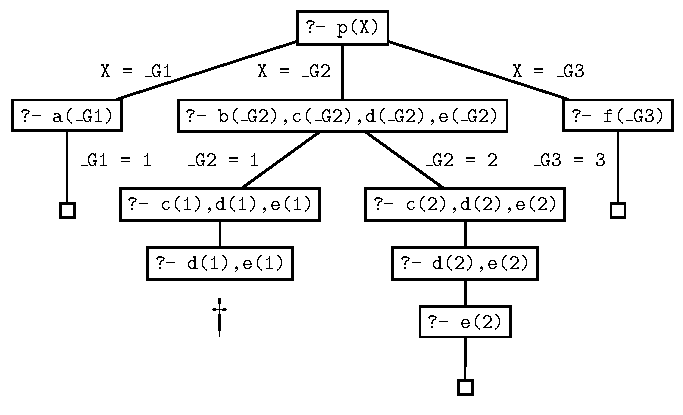
\includegraphics{chap10-pspic1.ps}
\end{center}

But now suppose we insert a cut in the second clause:
\begin{LPNcodedisplay}
p(X):- b(X), c(X), !, d(X), e(X).
\end{LPNcodedisplay}

If we now pose the query �p(X)� we will get the following
responses:
\begin{LPNcodedisplay}
X = 1 ;
no
\end{LPNcodedisplay}

What's going on here? Let's consider.

\begin{enumerate}

\item{}�p(X)� is first unified with the first rule, so we get a new
goal �a(X)�.  By instantiating �X� to �1�, Prolog unifies �a(X)� with
the fact �a(1)� and we have found a solution.  So far, this is exactly
what happened in the first version of the program.

\item{}We then go on and look for a second solution.  �p(X)� is
unified with the second rule, so we get the new goals
�b(X),c(X),!,d(X),e(X)�.  By instantiating �X� to �1�, Prolog unifies
�b(X)� with the fact �b(1)�, so we now have the goals
�c(1),!,d(1),e(1)�.  But �c(1)� is in the database so this simplifies
to �!,d(1),e(1)�.

\item{}Now for the big change.  The �!� goal succeeds (as it always
does) and commits us to the choices made so far.  In particular, we
are committed to having �X = 1�, and we are also committed to using
the second rule.

\item{}But �d(1)� fails.  And there's no way we can re-satisfy the
goal �p(X)�.  Sure, if we were allowed to try the value �X=2� we could
use the second rule to generate a solution (that's what happened in
the original version of the program).  But we \LPNemph{can't} do this:
the cut has removed this possibility from the search tree.  And sure,
if we were allowed to try the third rule, we could generate the
solution �X=3�.  But we \LPNemph{can't} do this: once again, the cut
has removed this possibility from the search tree.
\end{enumerate}

If you look at the search tree, you'll see that this all boils down to
the following: search stops when the goal �d(1)� doesn't lead to any
node where an alternative choice is available. The crosses in the
search tree indicate the branches that the cut  trimmed away.

\begin{center}
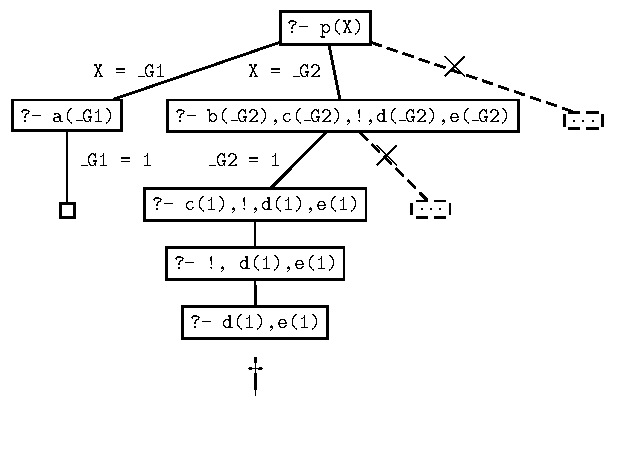
\includegraphics{chap10-pspic4.ps}
\end{center}

One point is worth emphasising: the cut only commits us to choices
made since the parent goal was unified with the left hand side of the
clause containing the cut.  For example, in a rule of the form
\begin{LPNcodedisplay}
q:- p1,...,pn, !, r1,...,rm
\end{LPNcodedisplay}
when we reach the cut it commits us to using this particular
clause for �q� and it commits us to the choices made when
evaluating �p1,...,pn�. However, we \LPNemph{are} free to backtrack
among the �r1,...,rm� and we are also free to backtrack among
alternatives for choices that were made before reaching the goal
�q�. A concrete example will make this clear.

First consider the following cut-free program:
\begin{LPNcodedisplay}
s(X,Y):- q(X,Y).
s(0,0).

q(X,Y):- i(X), j(Y).

i(1).
i(2).

j(1).
j(2).
j(3).
\end{LPNcodedisplay}

Here's how it behaves:
\begin{LPNcodedisplay}
?- s(X,Y).

X = 1
Y = 1 ;

X = 1
Y = 2 ;

X = 1
Y = 3 ;

X = 2
Y = 1 ;

X = 2
Y = 2 ;

X = 2
Y = 3 ;

X = 0
Y = 0;
no
\end{LPNcodedisplay}


And this is the corresponding search tree:


\begin{center}
\includegraphics{chap10-pspic5.ps}
\end{center}





Suppose we add a cut to the clause defining �q/2�:
\begin{LPNcodedisplay}
q(X,Y):- i(X), !, j(Y).
\end{LPNcodedisplay}

Now the program behaves as follows:
\begin{LPNcodedisplay}
?- s(X,Y).

X = 1
Y = 1 ;

X = 1
Y = 2 ;

X = 1
Y = 3 ;

X = 0
Y = 0;
no
\end{LPNcodedisplay}

Let's see why.

\begin{enumerate}

\item{}�s(X,Y)� is first unified with the first rule, which gives us a
new goal �q(X,Y)�.

\item{}�q(X,Y)� is then unified with the third rule, so we get the new
goals �i(X),!,j(Y)�.  By instantiating �X� to �1�, Prolog unifies
�i(X)� with the fact �i(1)�. This leaves us with the goal
�!,j(Y)�. The cut, of course, succeeds, and commits us to the choices
made so far.

\item{}But what are these choices?  These: that �X = 1�, and that
we are using this clause.  But note: we have \LPNemph{not} yet chosen a
value for �Y�.

\item{}Prolog then goes on, and by instantiating �Y� to �1�,
Prolog unifies �j(Y)� with the fact �j(1)�.  So we have
found a solution.

\item{}But we can find more.  Prolog \LPNemph{is} free to try another value
for �Y�. So it backtracks and sets �Y� to �2�, thus
finding a second solution.  And in fact it can find another solution:
on backtracking again, it sets �Y� to �3�, thus finding a
third solution.

\item{}But those are all alternatives for �j(X)�. Backtracking to
the left of the cut is not allowed, so it \LPNemph{can't} reset �X� to
�2�, so it won't find the next three solutions that the cut-free
program found. Backtracking over goals that were reached before
�q(X,Y)� is allowed however, so that Prolog will find the second
clause for �s/2�.
\end{enumerate}

Here's the corresponding search tree:

\begin{center}
\includegraphics{chap10-pspic6.ps}
\end{center}

\section{Using Cut}\label{SEC.L10.USING.CUT}

Well, we now know what cut is.  But how do we use it in practice, and
why is it so useful?  As a first example, let's define a (cut-free)
predicate �max/3� which takes integers as arguments\index{PROLOG max/3@\texttt{max/3}}
and succeeds if the third argument is the maximum of the first two.
For example, the queries
\begin{LPNcodedisplay}
?- max(2,3,3).
\end{LPNcodedisplay}

and
\begin{LPNcodedisplay}
?- max(3,2,3).
\end{LPNcodedisplay}

and
\begin{LPNcodedisplay}
?- max(3,3,3).
\end{LPNcodedisplay}

should succeed,
and the queries
\begin{LPNcodedisplay}
?- max(2,3,2).
\end{LPNcodedisplay}

and
\begin{LPNcodedisplay}
?- max(2,3,5).
\end{LPNcodedisplay}
should fail. And of course, we also want the program to work when the
third argument is a variable.  That is, we want the program to be able
to find the maximum of the first two arguments for us:
\begin{LPNcodedisplay}
?- max(2,3,Max).

Max = 3
yes

?- max(2,1,Max).

Max = 2
yes
\end{LPNcodedisplay}



Now, it is easy to write a program that does this. Here's
a first attempt:
\begin{LPNcodedisplay}
max(X,Y,Y):- X =< Y.
max(X,Y,X):- X>Y.
\end{LPNcodedisplay}
This is a perfectly correct program, and we might be tempted
simply to stop here. But we shouldn't: it's not good enough.

What's the problem? There is a potential inefficiency.  Suppose this
definition is used as part of a larger program, and somewhere along
the way �max(3,4,Y)� is called.  The program will correctly set �Y=4�.
But now consider what happens if at some stage backtracking is forced.
The program will try to re-satisfy �max(3,4,Y)� using the second
clause. This is completely pointless: the maximum of �3� and �4� is
�4� and that's that. There is no second solution to find.  To put it
another way: the two clauses in the above program are mutually
exclusive: if the first succeeds, the second must fail and vice versa.
So attempting to re-satisfy this clause is a complete waste of time.

With the help of cut, this is easy to fix. We need to insist that
Prolog should never try both clauses, and the following code does
this:
\begin{LPNcodedisplay}
max(X,Y,Y) :- X =< Y,!.
max(X,Y,X) :- X>Y.
\end{LPNcodedisplay}

Note how this works. Prolog will reach the cut if �max(X,Y,Y)� is
called and �X =< Y� succeeds. In this case, the second argument
is the maximum, and that's that, and the cut commits us to this
choice. On the other hand, if �X =< Y� fails, then Prolog goes
onto the second clause instead.

Note that this cut does \LPNemph{not} change the meaning of the
program.  Our new code gives exactly the same answers as the old one,
but it's more efficient.  In fact, the program is \LPNemph{exactly}
the same as the previous version, except for the cut, and this is a
pretty good sign that the cut is a sensible one. Cuts like this, which
don't change the meaning of a program, have a special name: they're
called \LPNterm{green cuts}.

But some readers will dislike this code. After all, isn't the second line
redundant? If we have to use this line, we already know that the first argument
is bigger that the second. Couldn't we squeeze out a little more efficiency
with the help of our new cut construct? Let's try. Here's a first (faulty)
attempt:
\begin{LPNcodedisplay}
max(X,Y,Y) :- X =< Y,!.
max(X,Y,X).
\end{LPNcodedisplay}
Note that is the same as our earlier green cut �max/3�, except that we have got
rid of the �>� test in the second clause.  How good is it?  Well, for some
queries it's fine. In particular, it answers correctly when we pose queries in
which the third argument is a variable. For example:
\begin{LPNcodedisplay}
?- max(100,101,X).

X = 101
yes
\end{LPNcodedisplay}

and
\begin{LPNcodedisplay}
?- max(3,2,X).

X = 3
yes
\end{LPNcodedisplay}

Nonetheless, it's \LPNemph{not} the same as the green cut program: the new
�max/3� does \LPNemph{not} work correctly. Consider what happens when all three arguments
are instantiated.  For example, consider the query
\begin{LPNcodedisplay}
?- max(2,3,2).
\end{LPNcodedisplay}
Obviously this query should fail.  But in our new version, it will
succeed!  Why? Well, this query simply won't unify with the head of
the first clause, so Prolog goes straight to the second clause. And
the query will unify with the second clause, and (trivially) the query
succeeds! So maybe getting rid of that �>� test wasn't quite so smart
after all.

But there is another way. The problem with the new code is simply that
we carried out variable unification \LPNemph{before} we traversed the
cut. Suppose we handle our variables a little more intelligently
(using three variables instead of two) and explicitly unify
\LPNemph{after} we have crossed the cut:
\begin{LPNcodedisplay}
max(X,Y,Z) :- X =< Y,!, Y = Z.
max(X,Y,X).
\end{LPNcodedisplay}
As the reader should check, this program does work, and (as we hoped
for) it avoids the explicit comparison made in the second clause of
our green cut version of �max/3�.

But there is an important difference between the new version of the
program and the green cut version.  The cut in the new program is a
classic example of what is known as a \LPNterm{red cut}.  As this
terminology is supposed to suggest, such cuts are potentially
dangerous.  Why?  Because if we take out such a cut, we
\LPNemph{don't} get an equivalent program. That is, if we remove the
cut, the resulting code does \LPNemph{not} compute the maximum of two
numbers any more. To put it another way, the presence of the cut is
\LPNemph{indispensable} to the correct functioning of the
program. (This was not the case in the  green cut version --- the
cut there merely
improved efficiency.) Because red cuts are
indispensable cuts, their presence means that programs containing them
are not fully declarative. Now, red cuts can be useful on occasions,
but beware!  Their use can lead to subtle programming mistakes and
make code hard to debug.

So, what to do? It's probably best to work as follows.  Try and get a
good, clear, cut-free program working, and only then try to improve
its efficiency by using cuts. Use green cuts whenever possible.  Red
cuts should be used only when absolutely necessary, and it's a good
idea to explicitly comment on any red cuts in your code. Working this
way will maximise your chances of striking a good balance between
declarative clarity and procedural efficiency.

\section{Negation as Failure}\label{SEC.L10.NEGATION.AS.FAILURE}

One of Prolog's most useful features is the simple way it lets us
state generalisations.  To say that Vincent enjoys burgers we just
write:
\begin{LPNcodedisplay}
enjoys(vincent,X) :- burger(X).
\end{LPNcodedisplay}

But in real life rules have exceptions.  Perhaps Vincent doesn't like
Big Kahuna burgers.  That is, perhaps the correct rule is really:
Vincent enjoys burgers, \LPNemph{except} Big Kahuna burgers.  Fine.
But how do we state this in Prolog?

As a first step, let's introduce another built-in predicate:
�fail/0�.  As its name suggests, �fail/0� is a special
symbol that will immediately fail when Prolog encounters it as a goal.
That may not sound too useful, but remember: \LPNemph{when Prolog fails, it
tries to backtrack}.  Thus �fail/0� can be viewed as an instruction
to force backtracking.  And when used in combination with cut, which
\LPNemph{blocks} backtracking, �fail/0� enables us to write some
interesting programs, and in particular, it lets us define exceptions
to general rules.


Consider the following code:
\begin{LPNcodedisplay}
enjoys(vincent,X) :- big_kahuna_burger(X),!,fail.
enjoys(vincent,X) :- burger(X).

burger(X) :- big_mac(X).
burger(X) :- big_kahuna_burger(X).
burger(X) :- whopper(X).

big_mac(a).
big_kahuna_burger(b).
big_mac(c).
whopper(d).
\end{LPNcodedisplay}

The first two lines describe Vincent's preferences.  The last six
lines describe a world containing four burgers, �a�, �b�,
�c�, and �d�.  We're also given information about what kinds of
burgers they are.  Given that the first two lines really do describe
Vincent's preferences (that is, that he likes all burgers except Big
Kahuna burgers) then he should enjoy burgers �a�, �c� and
�d�, but not �b�. And indeed, this is what happens:
\begin{LPNcodedisplay}
?- enjoys(vincent,a).
yes

?- enjoys(vincent,b).
no

?- enjoys(vincent,c).
yes

?- enjoys(vincent,d).
yes
\end{LPNcodedisplay}

How does this work?  The key is the combination of �!� and
�fail/0� in the first line (this even has a name: it's called the
\LPNterm{cut-fail combination}).  When we pose the query
�enjoys(vincent,b)�, the first rule applies, and we reach the
cut.  This commits us to the choices we have made, and in particular,
blocks access to the second rule.  But then we hit �fail/0�.  This
tries to force backtracking, but the cut blocks it, and so our query
fails.

This is interesting, but it's not ideal.  For a start, note that the
ordering of the rules is crucial: if we reverse the first two lines,
we \LPNemph{don't} get the behaviour we want.  Similarly, the cut is
crucial: if we remove it, the program doesn't behave in the same way
(so this is a \LPNemph{red} cut).  In short, we've got two mutually
dependent clauses that make intrinsic use of the procedural aspects of
Prolog.  Something useful is clearly going on here, but it would be
better if we could extract the useful part and package it in a more
robust way.

And we can.  The crucial observation is that the first clause is
essentially a way of saying that Vincent does \LPNemph{not} enjoy X if X
is a Big Kahuna burger.  That is, the cut-fail combination seems to be
offering us some form of negation.  And indeed, this is the crucial
generalisation: the cut-fail combination lets us define a form of
negation called \LPNterm{negation as failure}.  Here's how:
\begin{LPNcodedisplay}
neg(Goal) :- Goal,!,fail.
neg(Goal).
\end{LPNcodedisplay}
For any Prolog goal, �neg(Goal)� will succeed precisely if
�Goal� does \LPNemph{not} succeed.

Using our new �neg/1� predicate, we can describe Vincent's
preferences in a much clearer way:
\begin{LPNcodedisplay}
enjoys(vincent,X) :- burger(X),
                      neg(big_kahuna_burger(X)).
\end{LPNcodedisplay}
That is, Vincent enjoys X if X is a burger and X is not a Big Kahuna
burger.  This is quite close to our original statement: Vincent enjoys
burgers, except Big Kahuna burgers.

Negation as failure is an important tool.  Not only does it offer
useful expressivity (notably, the ability to describe exceptions) it
also offers it in a relatively safe form.  By working with negation as
failure (instead of with the lower level cut-fail combination) we have
a better chance of avoiding the programming errors that often
accompany the use of red cuts.  In fact, negation as failure is so
useful that it comes built-in as part of standard Prolog, so we don't
have to define it at all.  In standard Prolog the operator �\+� means
negation as failure, so we could define Vincent's preferences as
follows:
\begin{LPNcodedisplay}
enjoys(vincent,X) :- burger(X),
                      \+ big_kahuna_burger(X).
\end{LPNcodedisplay}


Nonetheless, a couple of words of warning are in order: \LPNemph{don't}
make the mistake of thinking that negation as failure works just like
logical negation.  It doesn't. Consider again our burger world:

\begin{LPNcodedisplay}
burger(X) :- big_mac(X).
burger(X) :- big_kahuna_burger(X).
burger(X) :- whopper(X).

big_mac(a).
big_kahuna_burger(b).
big_mac(c).
whopper(d).
\end{LPNcodedisplay}

If we pose the query �enjoys(vincent,X)� we get
the correct sequence of responses:
\begin{LPNcodedisplay}
X = a ;

X = c ;

X = d ;
no
\end{LPNcodedisplay}

But now suppose we rewrite the first line as follows:
\begin{LPNcodedisplay}
enjoys(vincent,X) :- \+ big_kahuna_burger(X), burger(X).
\end{LPNcodedisplay}
Note that from a declarative point of view, this should make no
difference: after all, \LPNemph{burger(x) and not big kahuna
burger(x)} is logically equivalent to \LPNemph{not big kahuna
burger(x) and burger(x)}.  That is, no matter what the variable
\LPNemph{x} denotes, it is impossible for one of these expressions to
be true and the other false.  Nonetheless, here's what happens
when we pose the same query:


\begin{LPNcodedisplay}
?- enjoys(vincent,X).

no
\end{LPNcodedisplay}




What's going on?  Well, in the modified database, the first thing that
Prolog has to check is whether �\+ big_kahuna_burger(X)� holds,
which means that it must check whether �big_kahuna_burger(X)�
fails.  But this succeeds. After all, the database contains the
information �big_kahuna_burger(b)�. So the query
�\+ big_kahuna_burger(X)� fails, and hence the original query
does too.  In a nutshell, the crucial difference between the two
programs is that in the original version (the one that works right) we
use �\+� only \LPNemph{after} we have instantiated the
variable �X�.  In the new version (which goes wrong) we use
�\+� before we have done this. The difference is crucial.

Summing up, we have seen that negation as failure is not logical
negation, and that it has a procedural dimension that must be
understood.  Nonetheless, it is an important programming construct: it
is generally a better idea to try use negation as failure than to
write code containing heavy use of red cuts.  Nonetheless,
``generally'' does not mean ``always''.  There \LPNemph{are} times
when it is better to use red cuts.


For example, suppose that we need to
write code to capture the following condition:
\LPNemph{p holds if a and b hold, or if a does not hold and c holds
too}. This can be captured with the help of negation
as failure very directly:

\begin{LPNcodedisplay}
p :- a,b.

p :- \+ a, c.
\end{LPNcodedisplay}

But suppose that �a� is a very complicated goal, a goal that
takes a lot of time to compute.  Programming it this way means we may
have to compute �a� twice, and this may mean that we have
unacceptably slow performance. If so, it would be better to use the
following program:

\begin{LPNcodedisplay}
p :- a,!,b.

p :- c.
\end{LPNcodedisplay}

Note that this is a red cut: removing it changes the meaning
of the program.

When all's said and done, there are no universal guidelines that will
cover all the situations you are likely to run across.  Programming is
as much an art as a science: that's what makes it so interesting.
You need to know as much as possible about the language you are
working with (whether it's Prolog, Java, Perl, or whatever), understand
the problem you are trying to solve, and know what counts as an
acceptable solution. And then: go ahead and try your best!




\section{Exercises}\label{SEC.L10.EXERCISES}

\begin{LPNexercise}{L10.EX1}Suppose we have the following database:
\begin{LPNcodedisplay}
p(1).
p(2) :- !.
p(3).
\end{LPNcodedisplay}

Write all of Prolog's answers to the following queries:
\begin{LPNcodedisplay}
?- p(X).

?- p(X),p(Y).

?- p(X),!,p(Y).
\end{LPNcodedisplay}
\end{LPNexercise}


\begin{LPNexercise}{L10.EX2}First, explain what the following program does:
\begin{LPNcodedisplay}
class(Number,positive) :- Number > 0.
class(0,zero).
class(Number,negative) :- Number < 0.
\end{LPNcodedisplay}

Second, improve it by adding green cuts.
\end{LPNexercise}


\begin{LPNexercise}{L10.EX3}Without using cut, write a predicate �split/3�
that splits a list of integers into two lists: one containing the
positive ones (and zero), the other containing the negative ones.  For
example:
\begin{LPNcodedisplay}
    split([3,4,-5,-1,0,4,-9],P,N)
\end{LPNcodedisplay}
should return:
\begin{LPNcodedisplay}
    P = [3,4,0,4]

    N = [-5,-1,-9].
\end{LPNcodedisplay}
Then improve this program, without changing its meaning, with the help
of the cut.
\end{LPNexercise}

\begin{LPNexercise}{L10.EX4}

Recall that in Exercise~\ref{L3.EX3} we gave you the following
knowledge base:
\begin{LPNcodedisplay}
directTrain(saarbruecken,dudweiler).
directTrain(forbach,saarbruecken).
directTrain(freyming,forbach).
directTrain(stAvold,freyming).
directTrain(fahlquemont,stAvold).
directTrain(metz,fahlquemont).
directTrain(nancy,metz).
\end{LPNcodedisplay}
We asked you to write a recursive predicate �travelFromTo/2� that
told us when we could travel by train between two towns.

Now, it's plausible to assume that whenever it is possible
to take a direct train from A to B, it is also possible to take a
direct train from B to A. Add this information to the database.
Then write a predicate  �route/3� which gives you a list of towns
that are visited by taking the train from one town to another.
For instance:

\begin{LPNcodedisplay}
?- route(forbach,metz,Route).
Route = [forbach,freyming,stAvold,fahlquemont,metz]
\end{LPNcodedisplay}

\end{LPNexercise}


\begin{LPNexercise}{L9.EX6}Recall the definition of jealousy given in Chapter~\ref{CHAPTER1}.
\begin{LPNcodedisplay}
jealous(X,Y):- loves(X,Z), loves(Y,Z).
\end{LPNcodedisplay}
In a world where both Vincent and Marsellus love Mia, Vincent will be
jealous of Marsellus, and Marsellus of Vincent. But Marsellus will
also be jealous of himself, and so will Vincent.  Revise the Prolog
definition of jealousy in such a way that people can't be jealous
of themselves.
\end{LPNexercise}




\section{Practical Session}\label{SEC.L10.PRAXIS}



The purpose of this session is to help you get familiar with cuts and
negation as failure.
First some keyboard exercises:

\begin{enumerate}
\item{}Try out all three versions of the
�max/3� predicate defined in the text: the cut-free
version, the green cut version, and the red cut version.  As usual,
``try out'' means ``run traces on'', and you should make sure that you
trace queries in which all three arguments are instantiated
to integers, and queries where the third argument is given as a
variable.
\item{}Ok, time for a burger. Try out all the methods discussed in the
text for coping with Vincent's preferences. That is, try out the
program that uses a cut-fail combination, the program that uses
negation as failure correctly, and also the program that mucks it up
by using negation in the wrong place.
\end{enumerate}


Now for some programming:

\begin{enumerate}
\item{}Define a predicate �nu/2� ("not unifiable") which takes two terms as
arguments and succeeds if the two terms do not unify.
For example:
\begin{LPNcodedisplay}
    nu(foo,foo).
    no

    nu (foo,blob).
    yes

    nu(foo,X).
    no
\end{LPNcodedisplay}

You should define this predicate in three different ways:
\begin{enumerate}
\item{}First (and easiest) write it with the help of �=� and
�\+�.
\item{}Second write it with the help of �=�, but don't use
�\+�.
\item{}Third, write it using a cut-fail combination. Don't use �=� and
don't use �\+�.
\end{enumerate}

\item{}Define a predicate �unifiable(List1,Term,List2)� where
�List2� is the list of all members of �List1� that unify with
�Term�.  The elements of �List2�
should \LPNemph{not} be instantiated by the unification.
For example
\begin{LPNcodedisplay}
    unifiable([X,b,t(Y)],t(a),List]
\end{LPNcodedisplay}

should yield
\begin{LPNcodedisplay}
    List = [X,t(Y)].
\end{LPNcodedisplay}

Note that �X� and �Y� are still \LPNemph{not} instantiated. So the tricky part
is: how do we check that they unify  with �t(a)� without instantiating them?

(Hint: consider using tests of the form �\+ term1 = term2�. Why?  Think
about it.  You might also like to think about tests of the form
�\+ \+ term1 = term2�.)
\end{enumerate}




\chapter{Database Manipulation and Collecting Solutions}\label{CHAPTER11}

\Thischapter{115}{

\noindent
This chapter has two main goals:

\begin{enumerate}

\item{}To discuss database manipulation in Prolog.

\item{}To discuss built-in predicates that let us collect all solutions to
        a problem into a single list.

\end{enumerate}

}



\section{Database Manipulation}\label{SEC.L11.DATABASE.MANIP}

Prolog has four database manipulation commands:
\LPNterm{assert},\index{PROLOG assert/1@\texttt{assert/1}}
\LPNterm{retract},\index{PROLOG retract/1@\texttt{retract/1}}
\LPNterm{asserta}, and
\LPNterm{assertz}.
Let's see how these are used.  Suppose we start with an empty database.  So if
we give the command:
\begin{LPNcodedisplay}
?- listing.
\end{LPNcodedisplay}
then Prolog will simply respond yes; the listing (of course) is empty.

Suppose we now give this command:
\begin{LPNcodedisplay}
?- assert(happy(mia)).
\end{LPNcodedisplay}

This succeeds (�assert/1� commands \LPNemph{always} succeed).  But
what is important is not that it succeeds, but the side-effect it has
on the database.  For if we now give the command
\begin{LPNcodedisplay}
?- listing.
\end{LPNcodedisplay}
we get:
\begin{LPNcodedisplay}
happy(mia).
\end{LPNcodedisplay}
That is, the database is no longer empty: it now contains the fact we
asserted.

Suppose we then made four more assert commands:
\begin{LPNcodedisplay}
?- assert(happy(vincent)).
yes

?- assert(happy(marcellus)).
yes

?- assert(happy(butch)).
yes

?- assert(happy(vincent)).
yes
\end{LPNcodedisplay}
and then ask  for a listing:
\begin{LPNcodedisplay}
?- listing.

happy(mia).
happy(vincent).
happy(marcellus).
happy(butch).
happy(vincent).
yes
\end{LPNcodedisplay}
All the facts we asserted are now in the knowledge base.  Note that
�happy(vincent)� is in the knowledge base twice. As we asserted
it twice, this seems sensible.

The database manipulations we have been making have changed the
meaning of the predicate �happy/1�.  More generally, database
manipulation commands give us the ability to change the meaning of
predicates while we are running programs.  Predicates whose
definitions change during run-time are called \LPNterm{dynamic
predicates}, as opposed to the \LPNterm{static predicates} that we have
previously dealt with.  Most Prolog interpreters insist that we
explicitly declare the predicates that we wish to be dynamic. We will
soon examine an example involving dynamic predicates, but let's first
complete our discussion of the database manipulation commands.


So far we have only asserted facts into the database, but we can also
assert new rules.  Suppose we want to assert the rule that
everyone who is happy is naive.  That is, suppose we want to assert
that:
\begin{LPNcodedisplay}
naive(X):- happy(X).
\end{LPNcodedisplay}
We can do this as follows:
\begin{LPNcodedisplay}
assert( (naive(X):- happy(X)) ).
\end{LPNcodedisplay}
Note the syntax of this command: \LPNemph{the rule we are asserting is
enclosed in a pair of brackets}.  If we now ask for a listing we get:
\begin{LPNcodedisplay}
happy(mia).
happy(vincent).
happy(marcellus).
happy(butch).
happy(vincent).

naive(A):-
   happy(A).
\end{LPNcodedisplay}


Now that we know how to assert new information into the database, we
should also learn how to remove information when we no longer need
it.  There is an inverse predicate to �assert/1�, namely �retract/1�.
For example, if we carry  straight on from the previous example
by giving  the command:
\begin{LPNcodedisplay}
?- retract(happy(marcellus)).
\end{LPNcodedisplay}
and then list the database, we get:
\begin{LPNcodedisplay}
happy(mia).
happy(vincent).
happy(butch).
happy(vincent).

naive(A) :-
    happy(A).
\end{LPNcodedisplay}
That is, the fact �happy(marcellus)� has been removed.

Suppose
we go on further, and say
\begin{LPNcodedisplay}
?- retract(happy(vincent)).
\end{LPNcodedisplay}
and then ask for a listing. We get:
\begin{LPNcodedisplay}
happy(mia).
happy(butch).
happy(vincent).

naive(A) :-
    happy(A).
\end{LPNcodedisplay}
Note that the first occurrence of �happy(vincent)�, and \LPNemph{only}
the first occurrence, was removed.

To remove all of our assertions contributing to the
definition of the predicate �happy/1� we can use a variable:
\begin{LPNcodedisplay}
?- retract(happy(X)).

X = mia ;

X = butch ;

X = vincent ;
no
\end{LPNcodedisplay}
A listing reveals that the database is now empty, except for the rule
�naive(A) :- happy(A)�.
\begin{LPNcodedisplay}
?- listing.
naive(A) :-
    happy(A).
\end{LPNcodedisplay}

\clearpage
If we want more control over where the asserted material is placed,
there are two variants of �assert/1�, namely:
\begin{enumerate}
\item{}\LPNterm{assertz}.  Places asserted material at the \LPNemph{end}\index{PROLOG assertz/1@\texttt{assertz/1}}
of the database.
\item{}\LPNterm{asserta}.  Places asserted material at the\index{PROLOG asserta/1@\texttt{asserta/1}}
\LPNemph{beginning} of the database.
\end{enumerate}

For example, suppose we start with an empty database, and then
we give the following command:
\begin{LPNcodedisplay}
assert( p(b) ), assertz( p(c) ), asserta( p(a) ).
\end{LPNcodedisplay}
Then a listing reveals that we now have the following
database:
\begin{LPNcodedisplay}
?- listing.

p(a).
p(b).
p(c).
yes
\end{LPNcodedisplay}

Database manipulation is a useful technique.  It is especially useful
for storing the results to computations, so that if we need to ask the
same question in the future, we don't need to redo the work: we just look
up the asserted fact. This technique is called \LPNterm{memoisation}, or
\LPNterm{caching}, and in some applications it can greatly increase
efficiency. Here's a simple example of this  technique at work:

\begin{LPNcodedisplay}
:- dynamic lookup/3.

add_and_square(X,Y,Res):-
   lookup(X,Y,Res), !.

add_and_square(X,Y,Res):-
   Res is (X+Y)*(X+Y),
   assert(lookup(X,Y,Res)).
\end{LPNcodedisplay}

What does this program do?  Basically, it takes two numbers X and Y,
adds X to Y, and then squares the result. For example we have:

\begin{LPNcodedisplay}
?- add_and_square(3,7,X).

X = 100
yes
\end{LPNcodedisplay}

But the important point is: \LPNemph{how} does it do this?  First,
note that we have declared �lookup/3� as a dynamic predicate.  We need
to do this as we plan to change the definition of �lookup/3�
during run-time.  Second, note that there are two clauses defining
�add_and_square/3�. The second clause performs the required arithmetic
calculation and asserts the result to the Prolog database using the
predicate �lookup/3� (that is, it  caches the result).  The first
clause checks the Prolog database to see if the calculation has
already been made in the past. If it has been, the program simply
returns the result, and the cut prevents it from entering the second
clause.

Here's an example of the program at work.
Suppose we give Prolog  another query
\begin{LPNcodedisplay}
?-  add_and_square(3,4,Y).

Y = 49
yes
\end{LPNcodedisplay}
If we now ask for a listing we see that the database now contains
\begin{LPNcodedisplay}
lookup(3, 7, 100).
lookup(3, 4, 49).
\end{LPNcodedisplay}
Should we later ask Prolog to add and square 3 and 4, it wouldn't
perform the calculations again. Rather, it would just return the
previously calculated result.

\medskip


Question: how do we remove all these new facts when we no longer want
them?  After all, if we give the command
\begin{LPNcodedisplay}
?- retract(lookup(X,Y,Z)).
\end{LPNcodedisplay}
Prolog will  go through all the facts one by one and ask us whether we want
to remove them!  But there's a much simpler way. Simply use the command\index{PROLOG retractall/3@\texttt{retractall/3}}
\begin{LPNcodedisplay}
?- retractall(lookup(_,_,_)).
\end{LPNcodedisplay}
This will remove all facts about �lookup/3� from the database.


To conclude our discussion of database manipulation, a word of
warning.  Although it is a useful technique, database manipulation
can lead to dirty, hard to understand, code.  If you use it heavily in
a program with lots of backtracking, understanding what is going on
can be a nightmare.  It is a non-declarative, non logical, feature of
Prolog that should be used cautiously.



\section{Collecting Solutions}\label{SEC.L11.COLLECTING.SOL}

There may be many solutions to a query. For example,
suppose we are working with the database
\begin{LPNcodedisplay}
child(martha,charlotte).
child(charlotte,caroline).
child(caroline,laura).
child(laura,rose).

descend(X,Y) :- child(X,Y).

descend(X,Y) :- child(X,Z),
                 descend(Z,Y).
\end{LPNcodedisplay}
Then if we pose the query
\begin{LPNcodedisplay}
descend(martha,X).
\end{LPNcodedisplay}
there are four solutions (namely �X=charlotte�, �X=caroline�,
�X=laura�, and �X=rose�).

However Prolog generates these solutions one by one.  Sometimes we
would like to have \LPNemph{all} the solutions to a query, and we
would like them handed to us in a neat, usable, form.  Prolog has
three built-in predicates that do this: \LPNterm{findall},
\LPNterm{bagof} and \LPNterm{setof}.  In essence, all these predicates
collect all the solutions to a query and put them in a single list ---
but there are important differences between them, as we shall see.



\subsection*{The {\tt findall/3} predicate}\label{SUBSEC.L11.FINDALL}


The query  \index{PROLOG findall/3@\texttt{findall/3}}
\begin{LPNcodedisplay}
?- findall(Object,Goal,List).
\end{LPNcodedisplay}
produces a list �List� of all the objects �Object� that
satisfy the goal �Goal�.  Often �Object� is simply a
variable, in which case the query can be read as: \LPNemph{Give me a list
containing all the instantiations of} �Object� \LPNemph{which satisfy}
�Goal�.

Here's an example.  Suppose we're working with the above
database (that is, with the information about �child� and the
definition of �descend�).  Then if we pose the query
\begin{LPNcodedisplay}
?- findall(X,descend(martha,X),Z).
\end{LPNcodedisplay}
we are asking for a list �Z� containing all the values of �X�
that satisfy �descend(martha,X)�. Prolog will respond
\begin{LPNcodedisplay}
X = _7489
Z = [charlotte,caroline,laura,rose]
\end{LPNcodedisplay}


But �Object� doesn't have to be a variable, it may be a complex term
that just contains
a variable that also occurs in �Goal�.  For example, we might decide that
we want to build a new predicate �fromMartha/1� that is true only
of descendants of Martha.  We could do this with the query:
\begin{LPNcodedisplay}
?- findall(fromMartha(X),descend(martha,X),Z).
\end{LPNcodedisplay}
That is, we are asking for a list �Z� containing all the instantiations of
�fromMartha(X)� that satisfy the goal �descend(martha,X)�.
Prolog will respond
\begin{LPNcodedisplay}
X = _7616
Z = [fromMartha(charlotte),fromMartha(caroline),
                 fromMartha(laura),fromMartha(rose)]
\end{LPNcodedisplay}


What happens if we ask the following query?
\begin{LPNcodedisplay}
?- findall(X,descend(mary,X),Z).
\end{LPNcodedisplay}
As there are no solutions for the goal �descend(mary,X)� in the
knowledge base.  �findall/3� returns an empty list.

Note that the first two arguments of �findall/3� typically have (at
least) one variable in common. When using �findall/3�, we normally
want to know what solutions Prolog finds for certain variables in the
goal, and we tell Prolog which variables in Goal we are interested in
by building them into the first argument of �findall/3�.

You might encounter situations, however, where �findall/3� does
useful work although the first two arguments don't share any
variables. For example, if you are not interested in who exactly is a
descendant of Martha, but only in how many descendants Martha has, you
can use the following query to find out:
\begin{LPNcodedisplay}
?- findall(Y,descend(martha,X),Z), length(Z,N).
\end{LPNcodedisplay}




\subsection*{The {\tt bagof/3} predicate}\label{SUBSEC.L11.BAGOF}

The �findall/3� predicate is useful, but in certain respects
it is rather crude. For example, suppose we pose the query
\begin{LPNcodedisplay}
?- findall(Child,descend(Mother,Child),List).
\end{LPNcodedisplay}
We get the response
\begin{LPNcodedisplay}
Child = _6947
Mother = _6951
List = [charlotte,caroline,laura,rose,caroline,
        laura,rose,laura,rose,rose]
\end{LPNcodedisplay}
Now, this is correct, but sometimes it would be useful if we had a
separate list for each of the different instantiations of �Mother�.

This is what �bagof/3� lets us do.  If we pose the query  \index{PROLOG bagof/3@\texttt{bagof/3}}
\begin{LPNcodedisplay}
?- bagof(Child,descend(Mother,Child),List).
\end{LPNcodedisplay}
we get the response
\begin{LPNcodedisplay}
Child = _7736
Mother = caroline
List = [laura,rose] ;

Child = _7736
Mother = charlotte
List = [caroline,laura,rose] ;

Child = _7736
Mother = laura
List = [rose] ;

Child = _7736
Mother = martha
List = [charlotte,caroline,laura,rose] ;
no
\end{LPNcodedisplay}

That is, �bagof/3� is more fine-grained than �findall/3�. It gives us the
opportunity to extract the information we want in a more structured
way.  Moreover, �bagof/3� can also do the same job as �findall/3�, with the
help of a special piece of syntax, namely �^�:
\begin{LPNcodedisplay}
?- bagof(Child,Mother^descend(Mother,Child),List).
\end{LPNcodedisplay}
This says: \LPNemph{give me a list of all the values of} �Child�
\LPNemph{such that} �descend(Mother,Child)�, \LPNemph{and put the result
in a list, but don't worry about generating a separate list for
each value of} �Mother�.  So posing this query yields:
\begin{LPNcodedisplay}
Child = _7870
Mother = _7874
List = [charlotte,caroline,laura,rose,caroline,
        laura,rose,laura,rose,rose]
\end{LPNcodedisplay}
Note that this is exactly the response that �findall/3� would have
given us. Still, if this is the
kind of query you want to make (and it often is) it's simpler to use
�findall/3�, because then you don't have to bother explicitly write
down the conditions using �^�.

There is one important difference between �findall/3�
and �bagof/3�, namely that �bagof/3� fails if the
goal that is specified in its second argument is not satisfied
(remember, that �findall/3� returns the empty list in such
cases). So the query
�bagof(X,descend(mary,X),Z)� yields �no�.

One final remark. Consider again the query
\begin{LPNcodedisplay}
?- bagof(Child,descend(Mother,Child),List).
\end{LPNcodedisplay}
As we saw above, this has four solutions. But, once again, Prolog
generates them one by one. Wouldn't it be nice if
we could collect them all into one list?

And we can. The simplest way is to use �findall/3�.  The query
\begin{LPNcodedisplay}
?- findall(List,
           bagof(Child,descend(Mother,Child),List),
           Z).
\end{LPNcodedisplay}
collects all of �bagof/3�'s responses into one list:
\begin{LPNcodedisplay}
List = _8293
Child = _8297
Mother = _8301
Z = [[laura,rose],[caroline,laura,rose],[rose],
                  [charlotte,caroline,laura,rose]]
\end{LPNcodedisplay}
Another way to do it is with �bagof/3�:
\begin{LPNcodedisplay}
?- bagof(List,
   Child^Mother^bagof(Child,descend(Mother,Child),List),
   Z).

List = _2648
Child = _2652
Mother = _2655
Z = [[laura,rose],[caroline,laura,rose],[rose],
                  [charlotte,caroline,laura,rose]]
\end{LPNcodedisplay}
This may not be the sort of thing you need to do very often, but
it does show the flexibility and power offered by these predicates.



\subsection*{The {\tt setof/3} predicate}\label{SUBSEC.L11.SETOF}

The �setof/3� predicate is basically the same as
�bagof/3�, but with one useful difference: the lists it contains
are \LPNemph{ordered} and contain \LPNemph{no redundancies} (that is,
no list contains repeated items).

For example, suppose we have the following database
\begin{LPNcodedisplay}
age(harry,13).
age(draco,14).
age(ron,13).
age(hermione,13).
age(dumbledore,60).
age(hagrid,30).
\end{LPNcodedisplay}

Now suppose we want a list of everyone whose
age is recorded in the database. We can do this
with the query:
\begin{LPNcodedisplay}
?- findall(X,age(X,Y),Out).

X = _8443
Y = _8448
Out = [harry,draco,ron,hermione,dumbledore,hagrid]
\end{LPNcodedisplay}


But maybe we would like the list to be ordered. We can achieve
this with the following query:\index{PROLOG setof/3@\texttt{setof/3}}
\begin{LPNcodedisplay}
?- setof(X,Y^age(X,Y),Out).
\end{LPNcodedisplay}
(Note that, just as with �bagof/3�, we have to tell �setof/3� not to
generate separate lists for each value of �Y�, and again we do
this with the �^� symbol.)
This query yields:
\begin{LPNcodedisplay}
X = _8711
Y = _8715
Out = [draco,dumbledore,hagrid,harry,hermione,ron]
\end{LPNcodedisplay}
Note that the list is alphabetically ordered.

Now suppose we are interested in collecting together all the ages
which are recorded in the database.  Of course, we could do this with the
following query:
\begin{LPNcodedisplay}
?- findall(Y,age(X,Y),Out).

Y = _8847
X = _8851
Out = [13,14,13,13,60,30]
\end{LPNcodedisplay}

But this output is rather messy. It is unordered and contains
repetitions.  By using �setof/3� we get the same information in a neater
form:
\begin{LPNcodedisplay}
?- setof(Y,X^age(X,Y),Out).

Y = _8981
X = _8985
Out = [13,14,30,60]
\end{LPNcodedisplay}


Between them, these three predicates offer us a great deal of
flexibility when it comes to collecting solutions.  For many purposes,
all we need is �findall/3�, but if we need more, �bagof/3� and
�setof/3� are there waiting to help us out.  But bear in mind that
there is an important difference between �findall/3� on the one hand
and �bagof/3� and �setof/3� on the other: �findall/3� will return an
empty list if the goal has no solutions, whereas �bagof/3� and
�setof/3� would fail in such a situation.


\section{Exercises}\label{SEC.L11.EXERCISES}

\begin{LPNexercise}{L11.EX1}Suppose we start with an empty database.
We then give the command:
\begin{LPNcodedisplay}
assert(q(a,b)), assertz(q(1,2)), asserta(q(foo,blug)).
\end{LPNcodedisplay}
What does the database now contain?

We then give the command:
\begin{LPNcodedisplay}
retract(q(1,2)), assertz( (p(X) :-  h(X)) ).
\end{LPNcodedisplay}
What does the database now contain?

We then give the command:
\begin{LPNcodedisplay}
retractall(q(_,_)).
\end{LPNcodedisplay}
What  does the database now contain?
\end{LPNexercise}


\begin{LPNexercise}{L11.EX2}Suppose we have the following database:
\begin{LPNcodedisplay}
q(blob,blug).
q(blob,blag).
q(blob,blig).
q(blaf,blag).
q(dang,dong).
q(dang,blug).
q(flab,blob).
\end{LPNcodedisplay}

What is Prolog's response to the queries:
\begin{LPNcodedisplay}
findall(X,q(blob,X),List).
findall(X,q(X,blug),List).
findall(X,q(X,Y),List).
bagof(X,q(X,Y),List).
setof(X,Y^q(X,Y),List).
\end{LPNcodedisplay}
\end{LPNexercise}


\begin{LPNexercise}{L11.EX3}Write a predicate �sigma/2� that takes an integer $n >
0$ and calculates the sum of all integers from 1 to
$n$. For example:

\begin{LPNcodedisplay}
?- sigma(3,X).
X = 6
yes
?- sigma(5,X).
X = 15
yes
\end{LPNcodedisplay}

Write the predicate so that results are stored in the database
(there should never be  more than one  entry in the database
for each value) and are reused whenever possible. For example,
suppose we make the following query:
\begin{LPNcodedisplay}
?- sigma(2,X).
X = 3
yes
?- listing.
sigmares(2,3).
\end{LPNcodedisplay}
Then, if we go on to ask
\begin{LPNcodedisplay}
?- sigma(3,X).
\end{LPNcodedisplay}
Prolog should not calculate everything new, but should get the result for
�sigma(2,3)� from the database and only add 3 to that. It should then answer:
\begin{LPNcodedisplay}
X = 6
yes
?- listing.
sigmares(2,3).
sigmares(3,6).
\end{LPNcodedisplay}
\end{LPNexercise}


\section{Practical Session}\label{SEC.L11.PRAXIS}

Try the following two programming exercises:

\begin{enumerate}
\item{}Sets can be thought of as lists that don't contain any repeated
elements.  For example, �[a,4,6]� is a set, but �[a,4,6,a]�
is not (as it contains two occurrences of �a)�. Write a Prolog
program �subset/2� that  is satisfied when the first
argument is a subset of the second argument (that is, when every
element of the first argument is a member of the second argument).
For example:
\begin{LPNcodedisplay}
?- subset([a,b],[a,b,c])
yes

?- subset([c,b],[a,b,c])
yes

?- subset([],[a,b,c])
yes
\end{LPNcodedisplay}

Your program should be capable of generating all subsets of an input set by
backtracking.  For example, if you give it as input
\begin{LPNcodedisplay}
?- subset(X,[a,b,c])
\end{LPNcodedisplay}
it should successively generate all eight subsets of �[a,b,c]�.
\item{}Using the �subset� predicate you have just written, and
�findall/3�, write a predicate �powerset/2� that takes a
set as its first argument, and returns the powerset of this set as the
second argument.  (The powerset of a set is the set of all its
subsets.) For example:
\begin{LPNcodedisplay}
?- powerset([a,b,c],P)
\end{LPNcodedisplay}
should return
\begin{LPNcodedisplay}
P = [[],[a],[b],[c],[a,b],[a,c],[b,c],[a,b,c]]
\end{LPNcodedisplay}
It doesn't matter if the sets are returned in some other
order. For example,
\begin{LPNcodedisplay}
P = [[a],[b],[c],[a,b,c],[],[a,b],[a,c],[b,c]]
\end{LPNcodedisplay}
is fine too.
\end{enumerate}




\chapter{Working With Files}\label{CHAPTER12}

\Thischapter{170}{

\noindent This chapter is concerned with various aspect of file handling and modularity.
We will learn three things:

\begin{enumerate}
\item{}How predicate definitions can be spread across different
        files.
\item{}How to write modular software systems.

\item{}How to write results to files and how to read input from
        files.
\end{enumerate}

}


\section{Splitting Programs over Files}\label{SEC.L12.SPLITTING.PROGRAMS}

By this stage you have written lots of programs that use the
predicates �append/3� and �member/2�. What you probably did each time
you needed one of them was to go back to the definition and copy it
over to the file where you wanted to use it. And maybe, after having
done that a few times, you started thinking that it was quite annoying
having to copy the same predicate definitions over and over again ---
how pleasant it would be if you could define them somewhere once and
for all and then simply access them whenever you needed them. Well,
that sounds like a pretty sensible thing to ask for and, of course,
Prolog offers you ways of doing it.



\subsection*{Reading in programs}\label{SUBSEC.L12.READING.PROGRAMS}

In fact, you already know a way of telling Prolog to read in predicate
definitions that are stored in a file, namely the
\begin{LPNcodedisplay}
[FileName1]
\end{LPNcodedisplay}
command. You have been using queries of this form all along to tell
Prolog to \LPNterm{consult} files. But there are two more useful things
you should know about it.  First, you can consult many files at once
by saying
\begin{LPNcodedisplay}
[FileName1,FileName2,...,FileNameN]
\end{LPNcodedisplay}
instead. Second, and more importantly,
file consultation does \textit{not} have
to be performed interactively. If you put
\begin{LPNcodedisplay}
:- [FileName1,FileName2,...,FileNameN].
\end{LPNcodedisplay}
at the top of your program file (say �main.pl�) you are telling Prolog
to first consult the listed files before going on to read in the rest
of your program.


This feature gives us a simple way of re-using definitions.  For
example, suppose that you keep all the predicate definitions for basic
list processing (such as �append/3�, �member/2�, �reverse/2�, and so
on) in a file called �listPredicates.pl�. If you want to use them,
simply put
\begin{LPNcodedisplay}
:- [listPredicates].
\end{LPNcodedisplay}
at the top of the file  containing the program that needs
them. Prolog will consult �listPredicates� when reading in that file,
and all the predicate definitions in �listPredicates� become
available.

There's one practical point you should be aware of. When Prolog loads
files, it doesn't normally check whether the files really need to be
consulted. If the predicate definitions provided by one of the files
are already in the database because that file was consulted
previously, Prolog will still consult it again, although it doesn't
need to. This can be annoying if you are consulting very large
files.

The built-in predicate
�ensure_loaded/1� behaves more intelligently  in this respect.  It
works as follows. On encountering the following
directive\index{PROLOG ensure_loaded/1@\texttt{ensure\_loaded/1}}
\begin{LPNcodedisplay}
:- ensure_loaded([listPredicates]).
\end{LPNcodedisplay}
Prolog checks whether the file �listPredicates.pl� has already been
loaded and only loads it again if it has changed since the last
loading.




\subsection*{Modules}\label{SUBSEC.L12.MODULES}

Now imagine that you are writing a program that manages a movie
database. You have designed a predicate �printActors� which displays
all actors starring in a particular film, and a predicate
�printMovies� which displays all movies directed by a particular
filmmaker. Both definitions are stored in different files, namely
�printActors.pl� and �printMovies.pl�, and both use an auxiliary
predicate �displayList/1�. Here's the first file:

\begin{LPNcodedisplay}
% This is the file: printActors.pl

printActors(Film):-
   setof(Actor,starring(Actor,Film),List),
   displayList(List).

displayList([]):- nl.
displayList([X|L]):-
   write(X), tab(1),
   displayList(L).
\end{LPNcodedisplay}
And here's the second:
\begin{LPNcodedisplay}
% This is the file: printMovies.pl

printMovies(Director):-
   setof(Film,directed(Director,Film),List),
   displayList(List).

displayList([]):- nl.
displayList([X|L]):-
   write(X), nl,
   displayList(L).
\end{LPNcodedisplay}

Note that �displayList/1� has different definitions in the two files:
the actors are printed in a row (using �tab/1�)\index{PROLOG tab/1@\texttt{tab/1}}, and the films are printed in a column (using
�nl/0�)\index{PROLOG nl/0@\texttt{nl/0}}.
Will this lead to conflicts in Prolog? Let's see. We'll
load both programs by placing the statements

\begin{LPNcodedisplay}
% This is the file: main.pl

:- [printActors].
:- [printMovies].
\end{LPNcodedisplay}
at the top of the main file. Consulting the main file will
evoke a message that  looks something like the
following:

\begin{LPNcodedisplay}
?- [main].
{consulting main.pl...}
{consulting printActors.pl...}
{printActors.pl consulted, 10 msec 296 bytes}
{consulting printMovies.pl...}
The procedure displayList/1 is being redefined.
    Old file: printActors.pl
    New file: printMovies.pl
Do you really want to redefine it? (y, n, p, or ?)
\end{LPNcodedisplay}

What has happened? Well, as both files �printActors.pl�
and �printMovies.pl�  define a predicate called �displayList/1�, Prolog
needs to choose one of the two definitions (it can't have two different
definitions for one predicate in its knowledge base).

What to do? Well, perhaps in some of these situations you really do
want to redefine a predicate.  But here you don't --- you want two
different definitions because you want movies and actors to be
displayed differently.  One way of dealing with this is to give a
different name to one of the two predicates.  But let's face it, this
is clumsy. You want to think of each file as a conceptually
self-contained entity; you don't want to waste time and energy
thinking about how you named predicates in some other file.  And the
most natural way of achieving the desired conceptual independence is
to use Prolog's \LPNterm{module system}.

Modules essentially allow you to hide predicate definitions. You are
allowed to decide which predicates should be \LPNterm{public} (that is,
callable from parts of the program that are stored in other files)
and which predicates should be \LPNterm{private} (that is, callable
only from within the module itself).  Thus you will not be able to
call private predicates from outside the module in which they are
defined, but there will be no conflicts if two modules internally
define the same predicate. In our example,  �displayList/1� is a good
candidate for becoming a private predicate; it plays a simple
auxiliary role in  both �printActors/1� and  �printMovies/1,�
and the  details of the
role it plays for one predicate are not relevant to the other.

You can turn a file into a module by putting a \LPNterm{module declaration} at
the top. Module declarations are of the form   \index{PROLOG module/2@\texttt{module/2}}

\begin{LPNcodedisplay}
:- module(ModuleName,
          List_of_Predicates_to_be_Exported).
\end{LPNcodedisplay}
Such declarations  specify the name of the module and the list of public
predicates, that is, the list of predicates that you want to
\LPNterm{export}. These will be the only predicates that are
accessible from outside the module.

Let's modularise our movie database programs. We only need to
include the following line at the top of the first file:

\begin{LPNcodedisplay}
% This is the file: printActors.pl

:- module(printActors,[printActors/1]).

printActors(Film):-
   setof(Actor,starring(Actor,Film),List),
   displayList(List).

displayList([]):- nl.
displayList([X|L]):-
   write(X), tab(1),
   displayList(L).
\end{LPNcodedisplay}
Here we have introduced a module called �printActors�,
with one public predicate �printActors/1�. The predicate
�displayList/1� is only known in the scope of the module
�printActors�, so its definition won't affect any other
modules.

Likewise we can turn the second file into a module:

\begin{LPNcodedisplay}
% This is the file: printMovies.pl

:- module(printMovies,[printMovies/1]).

printMovies(Director):-
   setof(Film,directed(Director,Film),List),
   displayList(List).

displayList([]):- nl.
displayList([X|L]):-
   write(X), nl,
   displayList(L).
\end{LPNcodedisplay}
Again, the  definition of the
�displayList/1� is only known in the scope of the module
�printMovies�, so there won't be any
clash when loading both modules at the same time.

Modules can be loaded with the built-in predicates �use_module/1�.
This will \LPNterm{import} all predicates that were defined as public
by the module. In other words, all public predicates will be\index{PROLOG use_module/1@\texttt{use\_module/1}}
accessible. To do this we need to change the main file as follows:

\begin{LPNcodedisplay}
% This is the file: main.pl

:- use_module(printActors).
:- use_module(printMovies).
\end{LPNcodedisplay}

If you don't want to use all public predicates of a module, but only
some of them, you can use the two-place version of �use_module�, which
takes a list of predicates that you actually want to import as its
\index{PROLOG use_module/2@\texttt{use\_module/2}} second argument.
So, by putting

\begin{LPNcodedisplay}
% This is the file: main.pl

:- use_module(printActors,[printActors/1]).
:- use_module(printMovies,[printMovies/1]).
\end{LPNcodedisplay}
at the top of the main file, we have explicitly stated that we
can use �printActors/1� and �printMovies/1�, and nothing else (in this
case, of course, the declaration is unnecessary as there are no other
public predicates that we could use).  Needless to say, you can only
import predicates that are actually exported by the relevant module.



\subsection*{Libraries}\label{SUBSEC.L12.LIBRARIES}

Many of the most common predicates are provided predefined, in one way
or another, by most Prolog implementations.  If you have been using
SWI Prolog, for example, you will probably have noticed that
predicates like �append/3� and �member/2� come as part of the
system. That's a speciality of SWI, however. Other Prolog
implementations, like SICStus for example, don't have them built-in,
but  provide them as part of a \LPNterm{library}.

Libraries are modules defining common predicates, and can be loaded
using the normal commands for importing modules. When specifying the
name of the library that you want to use, you have to tell Prolog that
this module is a library, so that Prolog knows where to look for it
(namely, in the place where Prolog keeps its libraries, not in the
directory where your other code is).
For example, putting the directive
\begin{LPNcodedisplay}
:- use_module(library(lists)).
\end{LPNcodedisplay}
at the top of your file tells Prolog to load a
library called �lists�. In SICStus Prolog, this library contains a set of
commonly used list processing predicates.

Libraries can be very useful and they can save you a lot of
work. Moreover, the code in libraries has typically been written by
excellent programmers, and is likely to be highly efficient and
problem-free.  However the way that libraries are organised and the
inventory of predicates provided by libraries are by no means
standardised across different Prolog implementations. This means that
if you want your program to run with different Prolog implementations,
it is probably easier and faster to define your own library modules
(using the techniques that we saw in the last section) rather
than to try to work around the incompatibilities between the library
systems of different Prolog implementations.



\section{Writing to Files}\label{SEC.L12.FILE.WRITING}

Many applications require that output be written to a file rather than
to the screen. In this section we will explain how to do this in
Prolog.

In order to write to a file we have to create one (or open an existing
one) and associate a \LPNterm{stream} with it. You can think of streams
as connections to files. In Prolog, streams are blessed with names in
a rather user-unfriendly format, such as
�'\$stream'(183368)�. Luckily, you never have to bother about the
exact names of streams --- although Prolog assigns these names
internally, you can use Prolog's unification to match the name to a
variable and make use of the variable rather than the name of the
stream itself.

Say you want to print the string 'Hogwarts' to the file �hogwarts.txt�.
This is done as follows:
\index{PROLOG open/3@\texttt{open/3}}
\index{PROLOG write/2@\texttt{write/2}}
\index{PROLOG close/1@\texttt{close/1}}
\index{PROLOG nl/1@\texttt{nl/1}}

\begin{LPNcodedisplay}
   ...
   open('hogwarts.txt',write,Stream),
   write(Stream,'Hogwarts'), nl(Stream),
   close(Stream),
   ...
\end{LPNcodedisplay}

What's happening here? Well, first the built-in predicate �open/3� is
used to create the file �hogwarts.txt�. The second argument of
�open/3� indicates that we want to \LPNterm{open} a new file
(overwriting any existing file with the same name). The third argument
of �open/3� returns the name of the stream. Secondly, we
\LPNterm{write} 'Hogwarts' on the stream and issue a newline command as
well. After this we are ready, and \LPNterm{close} the stream, using
the built-in �close/1�.

And that's more or less all there is to it.  As promised, we were not
interested in the name of the stream --- we used the variable �Stream�
to pass it around. Also note that the �write/2� predicate we used here
is basically a more general form of the �write/1� predicates we used
in Chapter~\ref{CHAPTER9} for writing to the screen.

What if you don't want to overwrite an existing file but
\LPNterm{append} to an existing one? This is done by choosing a
different mode when opening the file: instead of �write�, use �append�
as value for the second argument of �open/3�.  If a file of the
given name doesn't exist, it will be created.






\section{Reading from Files}\label{SEC.L12.FILE.READING}

In this section we show how to read from files.  Reading information
from files is straightforward in Prolog --- or at least, it is if this
information is given in the form of Prolog terms followed
by full stops. Consider the file �houses.txt�:

\begin{LPNcodedisplay}
gryffindor.
hufflepuff.
ravenclaw.
slytherin.
\end{LPNcodedisplay}
Here is a Prolog program that opens this file, reads\index{PROLOG read/2@\texttt{read/2}}\index{PROLOG open/3@\texttt{open/3}}
the information from it, and displays it on the screen:

\begin{LPNcodedisplay}
main:-
   open('houses.txt',read,Str),
   read(Str,House1),
   read(Str,House2),
   read(Str,House3),
   read(Str,House4),
   close(Str),
   write([House1,House2,House3,House4]), nl.
\end{LPNcodedisplay}
This opens a file in \LPNterm{reading mode}, then reads
four Prolog terms using the built-in predicate �read/2�,
closes the stream, and prints the information as a list.

All very straightforward. Nonetheless, the �read/2� predicate needs to
be handled with care. First of all, it only is able to handle Prolog
terms (we'll say more about this problem shortly). And secondly, it
will cause a run-time error if we use it to read from a stream when
there is nothing to read. Is there an elegant way to overcome this
second problem?

There is. The built-in predicate �at_end_of_stream/1� checks whether
the \LPNterm{end of a stream} has been reached, and can be
used as a safety-net.  For a stream �X�, �at_end_of_stream(X)�
will\index{PROLOG at_end_of_stream/1@\texttt{at\_end\_of\_stream/1}}
evaluate to true  when the end of the stream �X� is reached (in other
words, when all terms in the corresponding file have been read).

The following code is a modified version of our earlier reading-in
program, which shows how �at_end_of_stream/1� can be incorporated:

\begin{LPNcodedisplay}
main:-
   open('houses.txt',read,Str),
   read_houses(Str,Houses),
   close(Str),
   write(Houses), nl.

read_houses(Stream,[]):-
   at_end_of_stream(Stream).

read_houses(Stream,[X|L]):-
   \+ at_end_of_stream(Stream),
   read(Stream,X),
   read_houses(Stream,L).
\end{LPNcodedisplay}

Now for the nastier problem.  Recall that �read/2� only reads in
Prolog terms. If you want to read in arbitrary input, things become
rather unpleasant, as Prolog forces you to read information on the
level of characters.  The predicate that you need in this case is
�get_code/2� which\index{PROLOG get\_code/2@\texttt{get\_code/2}} reads the next
available character from a stream.  Characters are represented in
Prolog by their integer codes. For example, �get_code/2� will return �97�
if the next character on the stream is an �a�.

Usually we are not interested in these integer codes, but in the
characters --- or rather, in the atoms that are made up of lists of
these characters. How do we get our hands on these (lists of)
characters? One way is to use the built-in predicate �atom_codes/2�
that\index{PROLOG atom\_codes/2@\texttt{atom\_codes/2}} we introduced in
Chapter~\ref{CHAPTER9} to convert a list of integers into the
corresponding atom. We'll use this technique in the following example,
a predicate that reads in a word from a
stream.

\begin{LPNcodedisplay}
readWord(InStream,W):-
   get_code(InStream,Char),
   checkCharAndReadRest(Char,Chars,InStream),
   atom_codes(W,Chars).


checkCharAndReadRest(10,[],_):- !.

checkCharAndReadRest(32,[],_):- !.

checkCharAndReadRest(-1,[],_):- !.

checkCharAndReadRest(end_of_file,[],_):- !.

checkCharAndReadRest(Char,[Char|Chars],InStream):-
   get_code(InStream,NextChar),
   checkCharAndReadRest(NextChar,Chars,InStream).
\end{LPNcodedisplay}

How does this work?  It reads in a character and then checks whether
this character is a blank (integer code 32), a new line (10) or the
end of the stream ($-1$). In any of these cases a complete word has been
read, otherwise the next character is read.


\section{Exercises}\label{SEC.L12.EXERCISES}

\begin{LPNexercise}{L12.EX1}
Write code that creates  �hogwart.houses�, a file that  that looks
like this:
\begin{LPNcodedisplay}
       gryffindor
hufflepuff     ravenclaw
       slytherin
\end{LPNcodedisplay}
You can use the built-in predicates �open/3�, �close/1�, �tab/2�,
�nl/1�, and �write/2�.
\end{LPNexercise}


\begin{LPNexercise}{L12.EX2}
Write a Prolog program that reads in a plain text file word by word,
and asserts all read words and their frequency into the Prolog database. You may use the
predicate �readWord/2� to read in words. Use a dynamic predicate
�word/2� to store the words, where the first argument is a word, and
the second argument is the frequency of that word.
\end{LPNexercise}



\section{Practical Session}\label{SEC.L12.PRAXIS}

In this practical session, we want to combine what we have learned
about file handling with some topics we met in earlier chapters. The
goal is to write a program for running a DCG grammar on a testsuite,
so that the performance of the grammar can be checked.

What is a testsuite? It is a file that contains lots of possible
inputs (and expected outputs) for some program. In this case, a
testsuite will be a file that has lists representing grammatical and
ungrammatical sentences, such as
�[the,woman,shoots,the,cow,under,the,shower]� or
�[him,shoots,woman]�. The test program should take this file, run the
grammar on each of the sentences, and store the results in another
file. We can then look at the output file to check whether the grammar
answered everywhere the way it should have. When developing grammars,
testsuites like this are extremely useful for making sure that any
modifications we make to the grammar don't have unwanted effects.



\subsection*{Step 1}\label{L12.PRAXIS.STEP1}

Take the DCG that you built in the practical session of
Chapter~\ref{CHAPTER8} and turn it into a module, exporting the
predicate �s/3�, that is, the predicate that lets you parse sentences and
returns the parse tree as its first argument.




\subsection*{Step 2}\label{L12.PRAXIS.STEP2}

In the practical session of Chapter~\ref{CHAPTER9}, you
had to write a program for pretty printing parse trees onto the
screen. Turn that into a module as well.



\subsection*{Step 3}\label{L12.PRAXIS.STEP3}

Now modify the program so that it prints the tree not to the
screen but to a given stream. That means that the predicate
�pptree� should now be a two-place predicate taking the Prolog
representation of a parse tree and a stream as arguments.




\subsection*{Step 4}\label{L12.PRAXIS.STEP4}

Import both modules into a file and define a two-place predicate
�test� which takes a list representing a sentence (such as
�[a,woman,shoots]�), parses it,  and writes the result to the file
specified by the second argument of �test�.
Check that everything is working as it should.



\subsection*{Step 5}\label{L12.PRAXIS.STEP5}

Finally, modify �test/2�, so that it takes a filename instead of a
sentence as its first argument, reads in the sentences given in the
file one by one, parses them, and writes the sentence as well as the
parsing result into the output file. For example, if your input file
looked like this:
\begin{LPNcodedisplay}
[the,cow,under,the,table,shoots].

[a,dead,woman,likes,he].
\end{LPNcodedisplay}

the output file should look something like this:
\begin{LPNcodedisplay}
[the, cow, under, the, table, shoots]

   s(
      np(
         det(the)
         nbar(
            n(cow))
         pp(
            prep(under)
            np(
               det(the)
               nbar(
                  n(table)))))
      vp(
         v(shoots)))


[a, dead, woman, likes, he]

no
\end{LPNcodedisplay}



\subsection*{Step 6}\label{L12.PRAXIS.STEP6}

Now (if you are in for some real Prolog hacking) try to write a module
that reads in sentences terminated by a full stop or a line break from
a file, so that you can give your testsuite as
\begin{LPNcodedisplay}
the cow under the table shoots .

a dead woman likes he .
\end{LPNcodedisplay}

instead of
\begin{LPNcodedisplay}
[the,cow,under,the,table,shoots].

[a,dead,woman,likes,he].
\end{LPNcodedisplay}


\subsection*{Step 7}\label{L12.PRAXIS.STEP7}

Make the testsuite environment more sophisticated, by adding
information to the input file about the expected output (in this case,
whether the sentences has a parse or not). Then modify the program so
that it checks whether the expected output matches the obtained
output.








% splitindex.perl        (creates a new names.idx and prolog.idx files)
% makeindex -s LPN.isty lpn.idx
% makeindex -s LPN.isty prolog.idx

%\renewcommand*{\indexname}{Author Index}
%\input{names.ind}

\cleardoublepage
\renewcommand*{\indexname}{\hfill Predicate Index}
\addcontentsline{toc}{chapter}{Predicate Index}
\pagestyle{bbpindex}
\thispagestyle{empty}
\input{prolog.ind}

\cleardoublepage
\renewcommand*{\indexname}{\hfill Subject Index}
\addcontentsline{toc}{chapter}{Subject Index}
\pagestyle{bbsindex}
\printindex


\newpage\thispagestyle{empty}\strut
\newpage\thispagestyle{empty}\strut
\newpage\thispagestyle{empty}\strut
\newpage\thispagestyle{empty}\strut
\newpage\thispagestyle{empty}\strut

\end{document}
